% class options:
% - select either [german] or [english]
% - select the type of thesis from:
%   [bachelor, master, generic]
%   (in case of generic, use \type{} to specify it)
% - use option "alpha" for abbreviated citation (instead of numbers)
% - option "draft" is available, too
% - use options "utf8" or "latin1" to select inputencoding
\documentclass[english, bachelor, utf8]{base/thesis_telematics}

% \usepackage{units}    % useful for settings units:              \unit[23]{m}
\usepackage{nicefrac} % for setting fractions esp. within text: \nicefrac{km}{h}
\usepackage{tabularx}
\usepackage{subcaption}
\usepackage{booktabs}
\usepackage{float}
\usepackage{siunitx}
\usepackage{threeparttable}
\usepackage{rotating}
\usepackage{url}
\usepackage{hyperref}
\usepackage[section]{placeins}
\usepackage{algorithm, algorithmic}  % for pseudo code (cf. documentation)
\renewcommand{\algorithmiccomment}[1]{\qquad{\small // \textit{#1}}}

%%%%%%%%%%%%%%%%%%%%%%%%%%%%%%%%%%%%%%%%%%%%%%%%%%%%%%%%%%%%%%%%%%%%%%%%%%%%%%%

\def\UrlBreaks{\do\/\do-}

\begin{document}

\title{3D Mapping with Rolling Spheres Using a Livox Mid-360 LiDAR}
\author{Marawan Salah Abdelrahman Khalil Khalil}
\email{marawan.abdelrahman@student.guc.edu.eg}
\firstSupervisor{Prof. Dr. Andreas Nüchter}
\secondSupervisor{}
\thirdSupervisor{M.Sc Fabian Arzberger}
%\thirdSupervisor{} %for to give credit to the person supervising but not reviewing the thesis 
%\dept{...}                             % by default Robotics and Telematics
%\submitdate{November 2004}             % by default current month & year
%\signcity{}                            % by default Würzburg
%signline{Würzburg, 1. April 2014} % by default "signcity, submitdate"

\generatetitle

\cleardoublepage    

\begin{prefacesection}{Acknowledgements}
I would like to thank God for granting me good health, strength, and blessings to complete this work.
I am deeply grateful to my family for their continuous support and encouragement throughout my academic journey.
I would also like to express my sincere gratitude to my supervisor, Prof. Dr. Andreas Nüchter, for giving me the opportunity to work on this exciting project, for his invaluable guidance and constructive feedback, and for providing the necessary resources and facilities to conduct this research.
I am especially thankful to Fabian Arzberger for his assistance, inspiring discussions, and the valuable time we spent together working on research development and improvements.
I would also like to thank Dr. Michael Bleier for his generous technical advice and support whenever I needed guidance.
I am grateful to my friends and colleagues at the Robotics Department for their encouragement and camaraderie.
Finally, I would like to thank my friends from Cairo and Würzburg for their unwavering support and friendship.
\end{prefacesection}

\newpage

\begin{prefacesection}{Abstract}
Spherical robots offer unique advantages for mapping applications in hazardous or confined environments, unlike traditional wheeled or legged robots, thanks to their protective shells and omnidirectional mobility. 
Recent research has focused on developing more robust motion mechanisms, and some have incorporated technologies like LiDAR for 3D mapping, further expanding their capabilities in complex and unpredictable environments. 
However, the rapid evolution of LiDAR–inertial algorithms and modern hardware platforms presents new opportunities for spherical SLAM, while the integration of actuation with mapping and localization remains largely unexplored.

To address this, this work presents two complementary spherical mapping systems: a light\-weight, non-actuated design and an actuated variant featuring internal pendulum-driven locomotion. 
Both systems are equipped with a Livox Mid-360 solid-state LiDAR sensor and run LiDAR-Inertial Odometry (LIO) algorithms in real-time on resource-constrained hardware (Raspberry Pi 5). 
We assess the mapping accuracy of these systems by comparing the resulting 3D point-clouds from the LIO algorithms to a ground truth map from a high-precision terrestrial laser scanner.
% The results indicate that the performance of state-of-the-art LIO algorithms deteriorates due to the high dynamic movement introduced by the spherical locomotion, leading to globally inconsistent maps and sometimes unrecoverable drift.
A comparative evaluation highlights distinct performance characteristics: the non-actuated sphere achieves higher mapping accuracy, while the actuated system provides denser point-clouds and shows potential for autonomous navigation. 
Furthermore, the performance of state-of-the-art LIO algorithms deteriorates due to the high dynamic movement introduced by the spherical locomotion, leading to globally inconsistent maps and sometimes unrecoverable drift.
%These results lay the groundwork for deploying spherical robots in challenging environments such as underground infrastructure or planetary surfaces, where traditional robotic platforms often face operational constraints. \dots
\end{prefacesection}
\cleardoublepage
\tableofcontents

\thispagestyle{empty}
\listoffigures
\listoftables
\newpage
\pagenumbering{arabic}

\startTextChapters %%%%%%%%%%%%%%%%%%%%%%%%%%%%%%

\chapter{Introduction}
\label{ch:introduction}

In recent decades, robotics has evolved from a niche discipline into a transformative technology impacting a wide range of industries, including manufacturing, healthcare, space exploration, and personal assistance. 
Among the diverse types of robotic systems, spherical robots have recently begun to attract increased attention from researchers. These robots represent a relatively unconventional design compared to more familiar, rotation-restricted systems such as UAVs, handheld devices, and wheeled vehicles. 
Unlike traditional wheeled or legged robots, spherical robots offer several key advantages, including omnidirectional movement, enhanced maneuverability in unpredictable environments, and improved protection for internal components. 
These features make them well-suited for a variety of applications such as surveillance, inspection, and environmental monitoring in hazardous conditions. 
Their spherical design enables them to access environments that are difficult or impossible for other robotic systems to navigate, such as steep tunnels, underground mines, narrow passageways, and other confined or dangerous spaces.
The sealed outer shell of a spherical robot provides full protection against dust, hazardous chemicals, liquids, and external impacts. 

Recent research has focused on developing more robust motion mechanisms~\cite{roboball,novelsphere,pendulum_sphere} and incorporating technologies like LiDAR for 3D mapping, further expanding their capabilities in complex and unpredictable environments~\cite{Kalman_filter_sphere,DAEDALUS,sphere_Fabi_1}.
However, the rapid evolution of LiDAR–inertial algorithms and modern hardware platforms presents new opportunities for spherical SLAM, while the integration of actuation with mapping and localization remains largely unexplored.
To address this, we present and evaluate two custom-built spherical robots (see Fig.~\ref{fig:twospheres}) equipped with LiDAR-based SLAM systems.
Both systems integrate FAST-LIO2~\cite{fastlio2}, FAST-LIVO2~\cite{fastlivo2}, and DLIO~\cite{dlio}, which are state-of-the-art LiDAR-inertial odometry algorithms.
The primary contribution of this work is the comparative analysis of these algorithms' performance on spherical platforms and their validation against terrestrial laser scanning ground truth data.
This evaluation provides insights into the practical applicability of different SLAM approaches for spherical robots and establishes benchmarks for future developments in this emerging field.

\begin{figure}[h]
\centerline{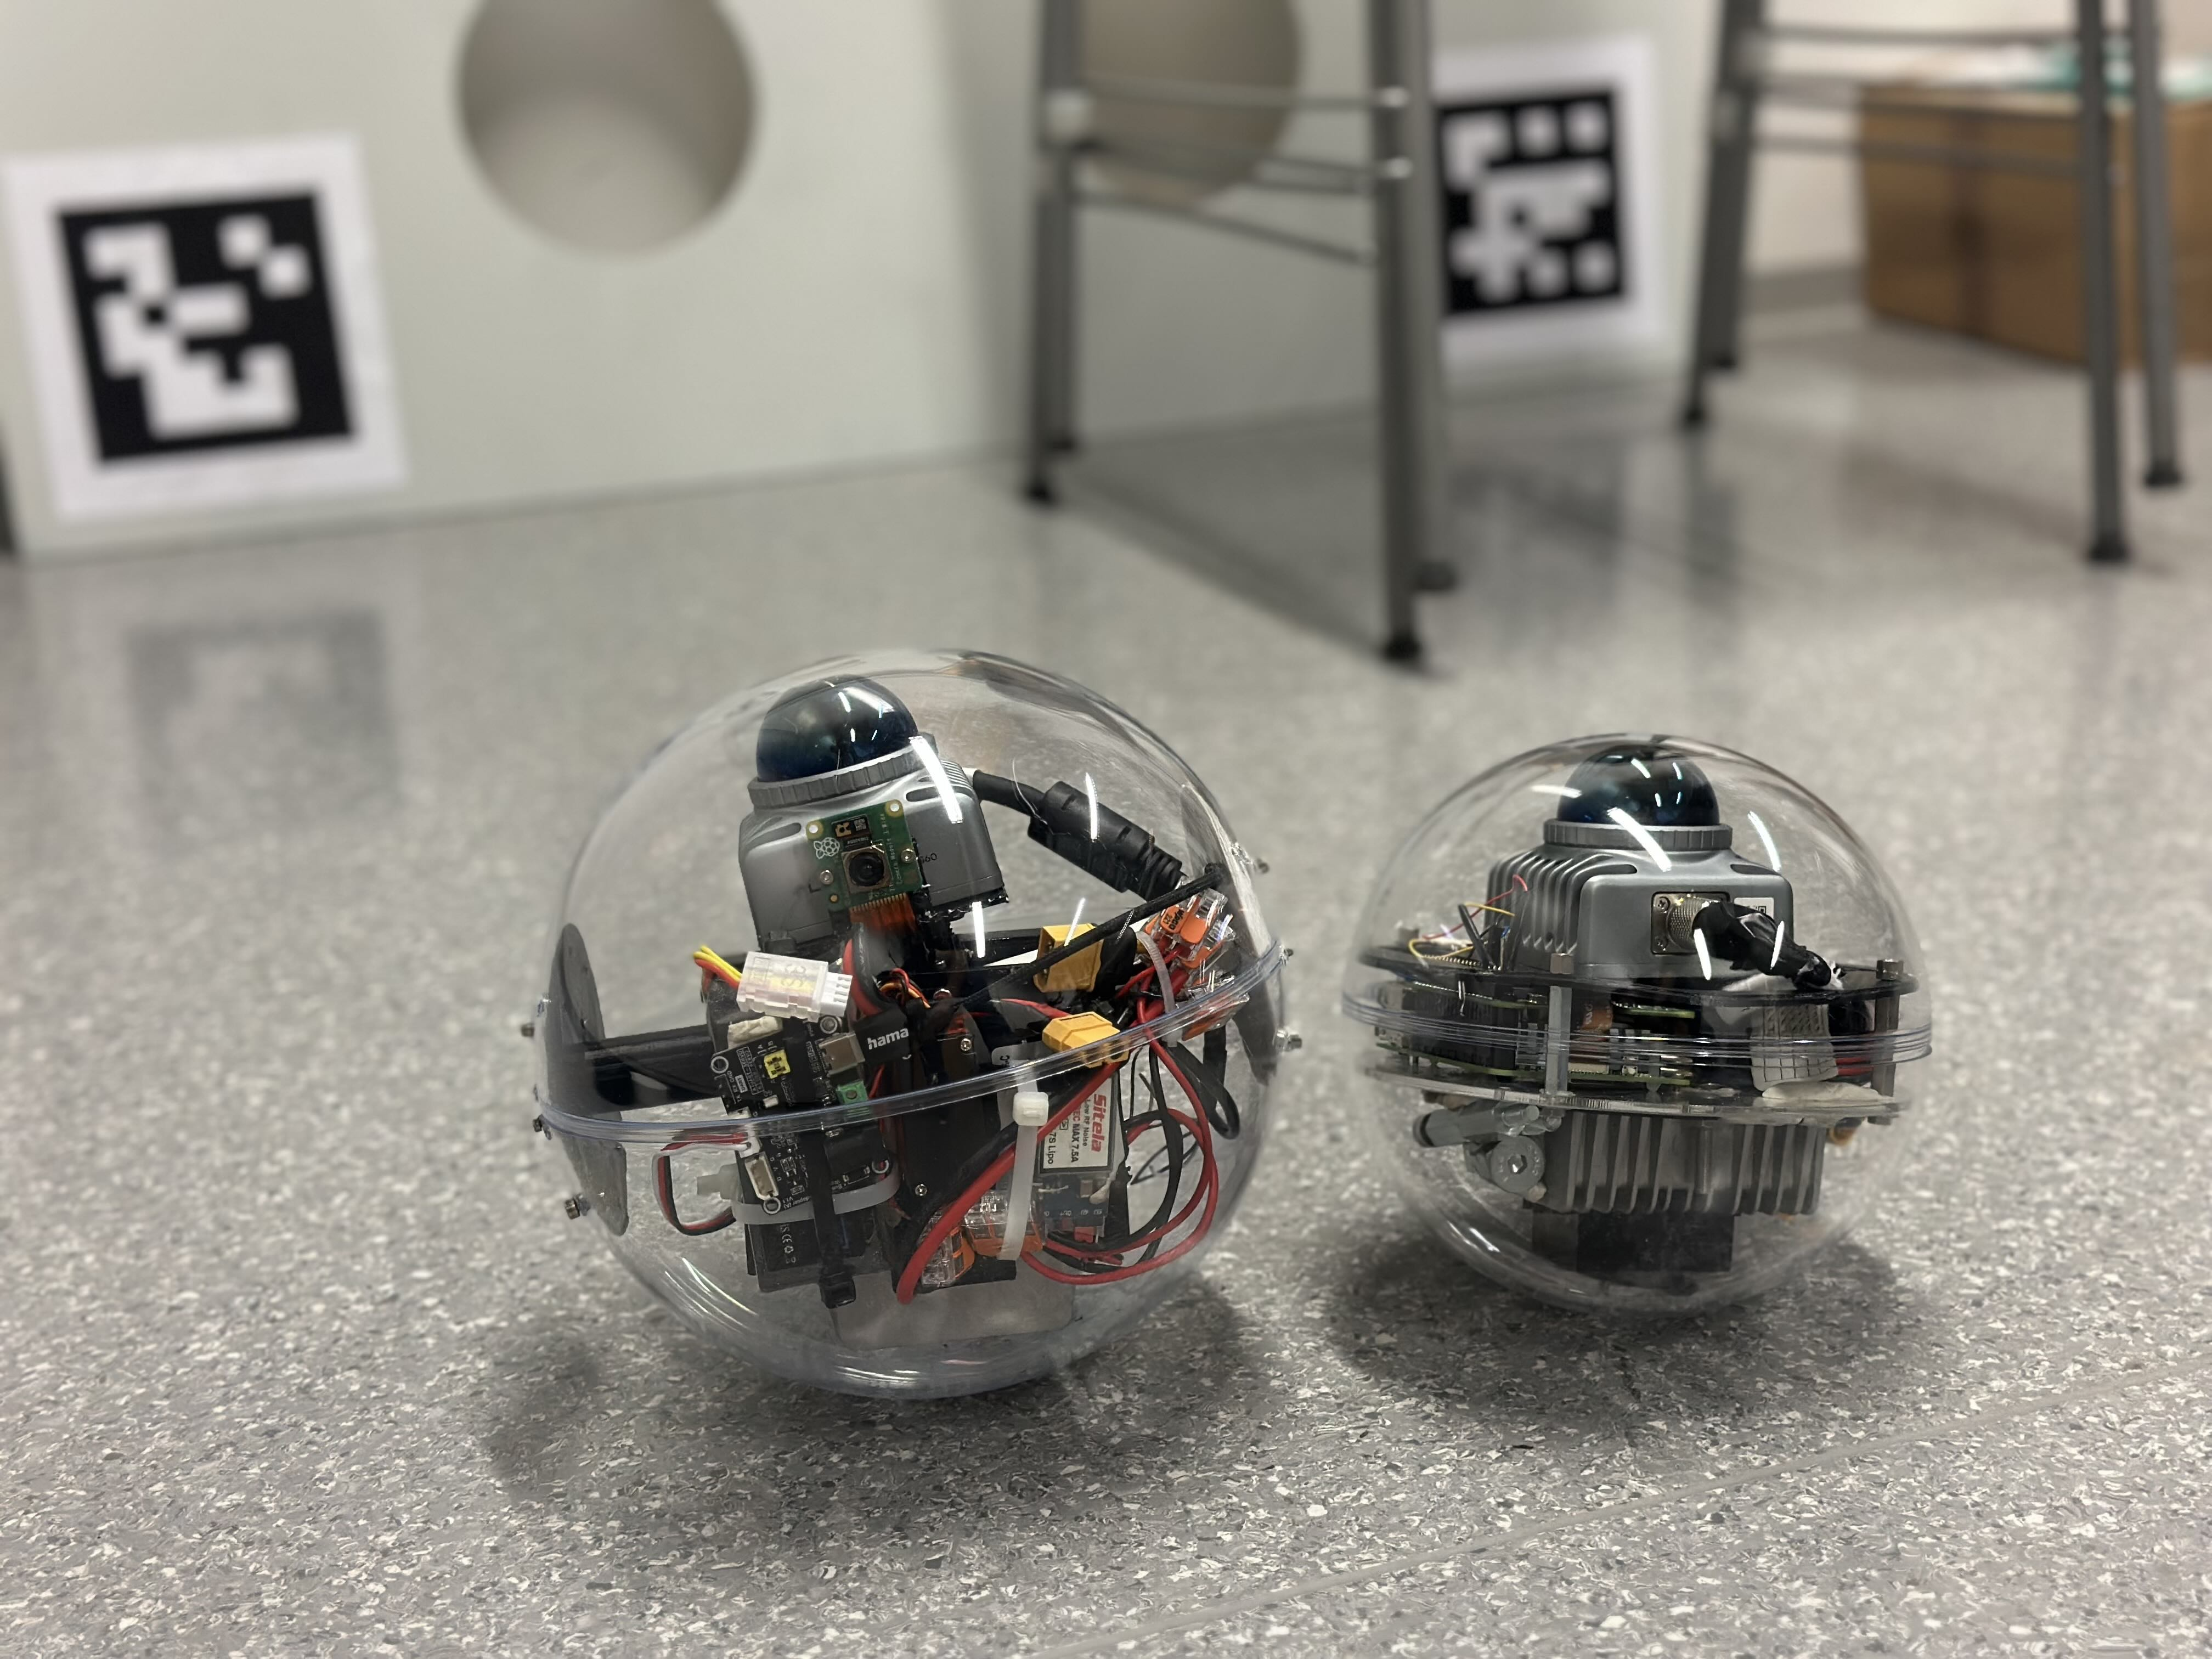
\includegraphics[width=0.8\columnwidth]{pics/two_spheres.jpg}}
\caption{(Left:) \SI{20}{\centi\meter} diameter actuated sphere.
(Right:) \SI{16}{\centi\meter} diameter non-actuated sphere.
A video where both spheres are moving is available at \url{https://youtube.com/shorts/lxTF85HK-zY}.}

\label{fig:twospheres}
\end{figure}

\begin{figure}[h]
\centerline{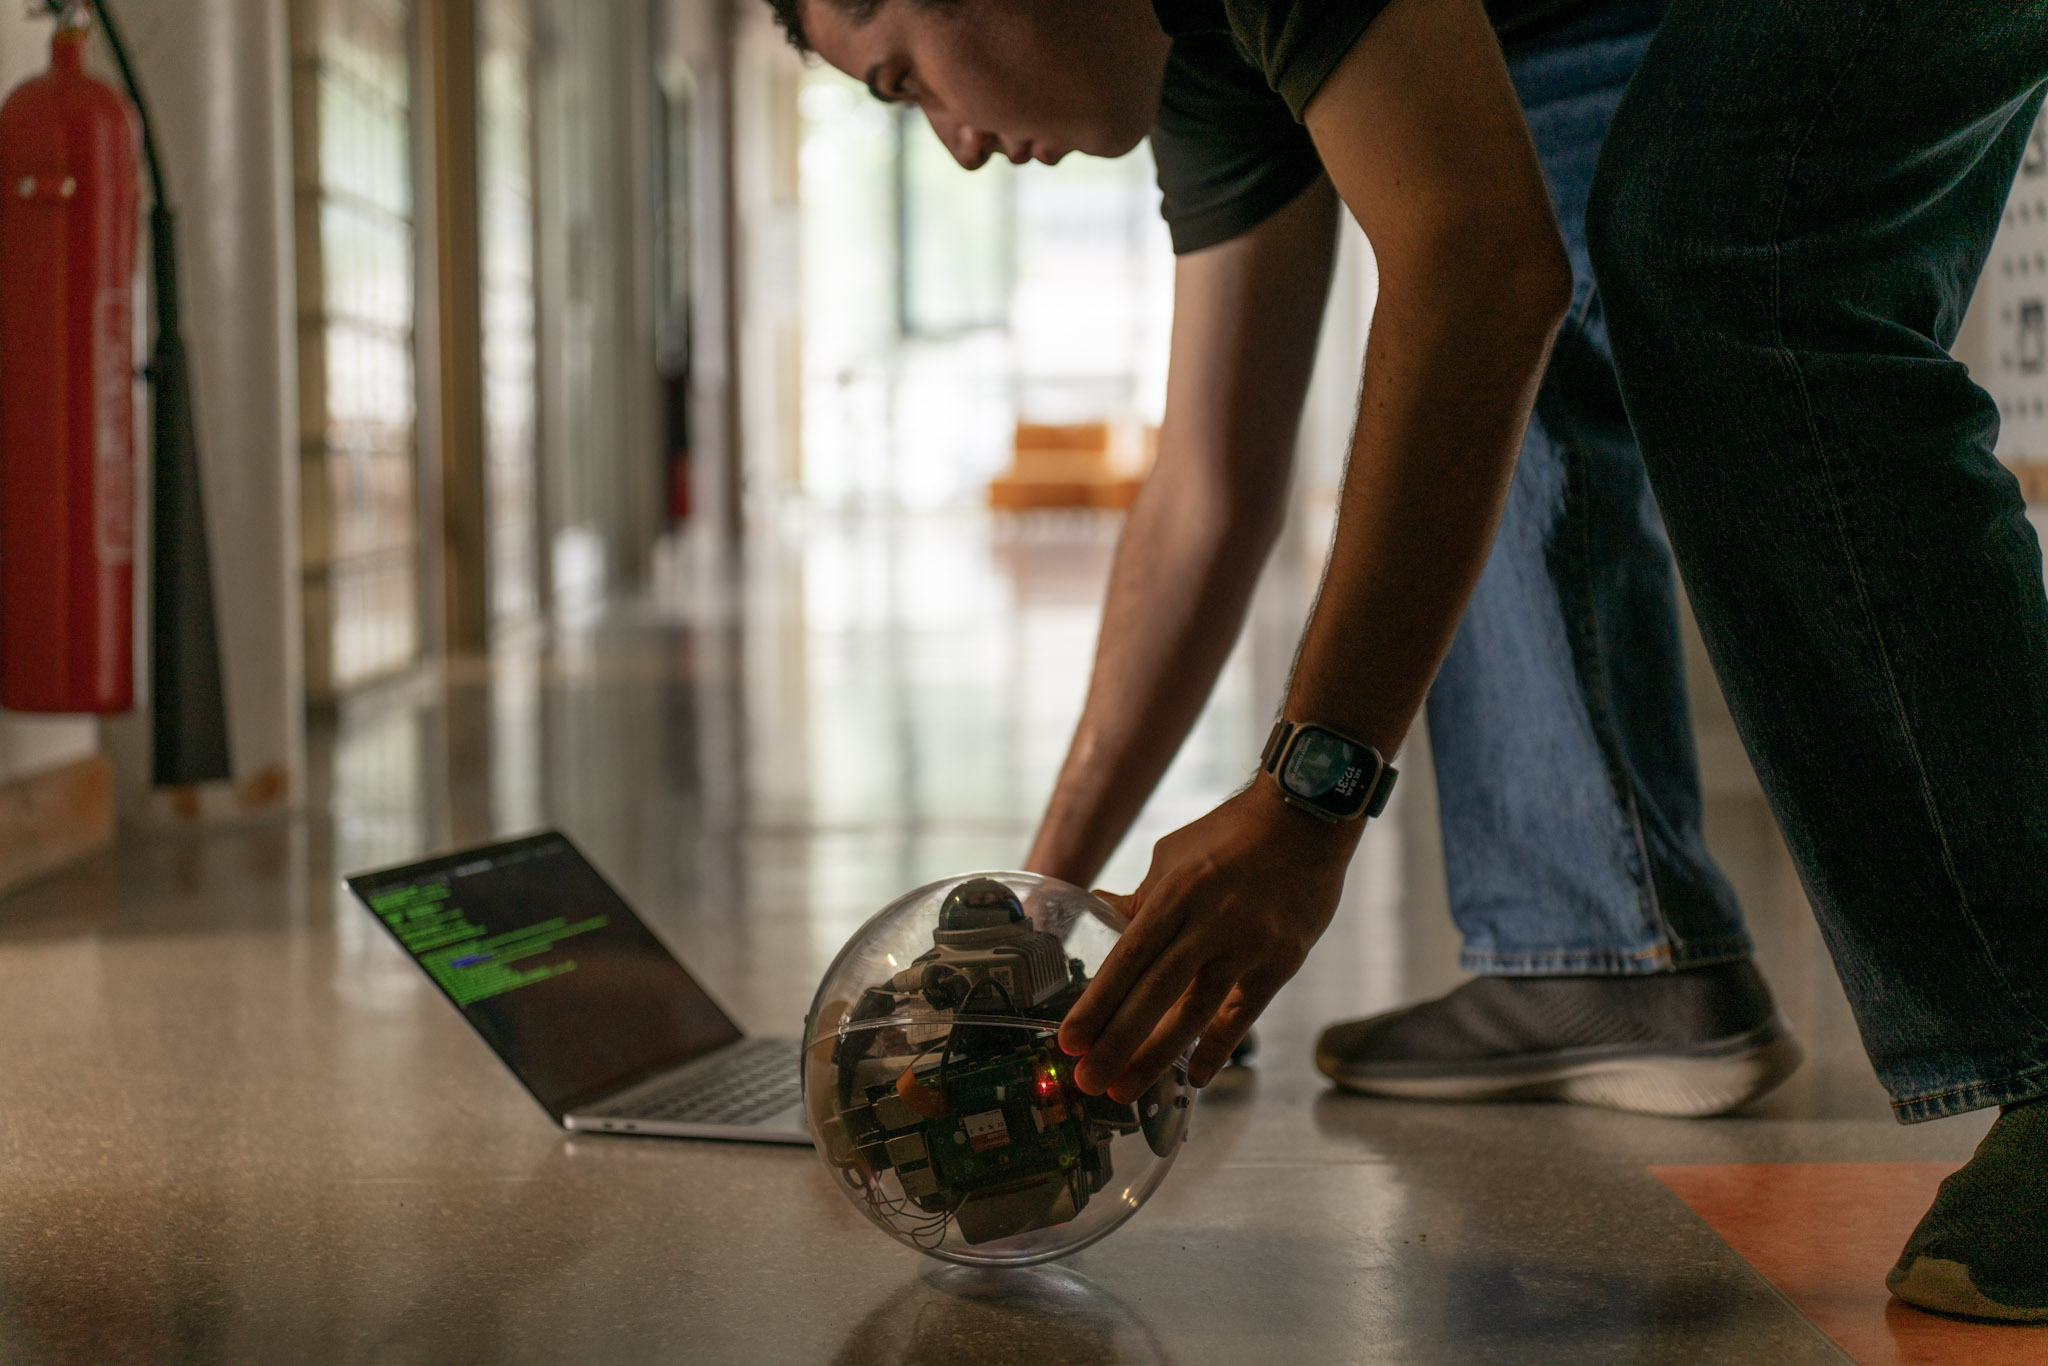
\includegraphics[width=0.8\columnwidth]{pics/marosphere_pic3.jpg}}
\caption{Actuated Sphere being tested and evaluated in Computer Science building at the University of Würzburg.}
\label{fig:test}
\end{figure}


\section{Outline}
In the next Chapter, we review recent SLAM developments for spherical platforms, with emphasis on LiDAR-inertial methods, followed by advancements in spherical robot design.
In Chapter~\ref{ch:fundamentals}, we provide an overview of the fundamental concepts and technologies that relates to our work, including Inertial Measurement Units (IMUs), LiDAR technology, spherical robot types, an introduction to SLAM and Control Strategies.
In Chapter~\ref{ch:hardwaredesign}, we provide a description of the hardware implementation of the two spherical robots. 
Subsequently, we describe the software integration, as well as the motion control mechanisms used for the actuated sphere. 
Finally, we provide a comprehensive evaluation of the mapping accuracy by comparing the maps of the proposed systems with a ground truth map obtained using high-precision terrestrial laser scanning (TLS). 


\chapter{State of the Art}
\label{ch:state-of-the-art}
This chapter reviews the current landscape of spherical robots, focusing on two critical aspects: SLAM algorithms adapted for rolling platforms and locomotion mechanisms that enable controlled motion. The unique constraints of spherical robots—enclosed sensors, aggressive rolling dynamics, and operation in confined spaces—drive both the algorithmic choices for perception and the mechanical strategies for mobility. Section~\ref{AA} surveys spherical SLAM with a focus on LiDAR–inertial methods. Section~\ref{sec:sphere-locomotion} reviews various locomotion mechanisms.

\section{Spherical SLAM}\label{AA}
Spherical Simultaneous Localization and Mapping (SLAM) is an emerging area within mobile robotics, offering promising solutions for robust mapping in constrained or hazardous environments. 
Unlike traditional platforms, spherical robots encapsulate their sensors within a protective shell and rely on rolling locomotion. 
This unique configuration introduces both opportunities and significant challenges for SLAM algorithms. 
One of the earliest spherical SLAM prototypes was L.U.N.A.~\cite{luna}, which employed a 2D LiDAR and IMU inside a rolling spherical shell. 
The design validated the feasibility of spherical SLAM. 
It also featured actuation through internal flywheels, using an IBCOAM (Impulse by Conservation of Angular Momentum) mechanism.

A major milestone in this field was the DAEDALUS project~\cite{DAEDALUS}, funded by the European Space Agency, which proposed a fully enclosed spherical robot for the autonomous exploration of lunar lava tubes. 
The robot was proposed to be equipped with LiDAR and internal actuators, and its design focused on resilience to lunar regolith and harsh environmental conditions.
A core challenge in spherical SLAM is the aggressive and off-centered rotation induced by rolling locomotion. 
These motions produce high angular velocities and dynamic behavior across all principal axes. 
This significantly degrades pose estimation accuracy and leads to error accumulation in the map. 
This problem is further compounded by the absence of magnetometer use—often intentionally excluded due to the unreliability of magnetic field data in planetary environments.
This leads to uncorrected yaw drift in IMU-based odometry, especially during prolonged navigation.

\begin{figure}[h]
    \centering
\begin{subfigure}{0.48\textwidth}
    \centering
    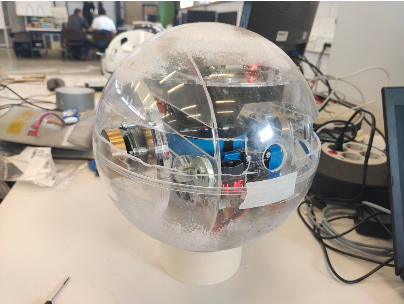
\includegraphics[width=0.9\textwidth]{pics/luna.png}
    \label{fig:luna_flywheel}
    \caption{L.U.N.A. robot with flywheel actuation~\cite{luna}.}
\end{subfigure}
\hfill
\begin{subfigure}{0.48\textwidth}
    \centering
    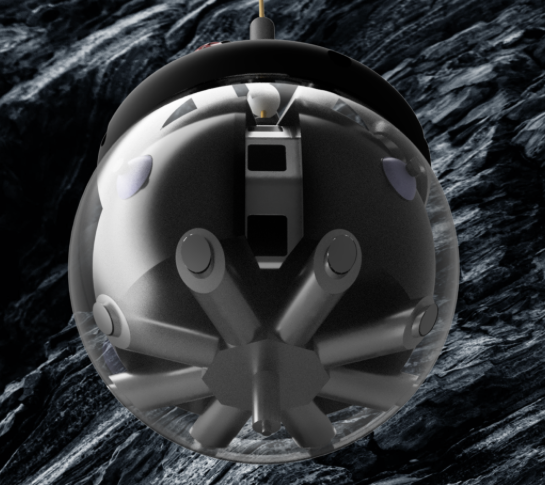
\includegraphics[width=0.8\textwidth]{pics/DAEDALUS.png}
    \label{fig:daedalus}
    \caption{DAEDALUS robot for lunar exploration~\cite{esa_lunar_cave_explorer}.}
\end{subfigure}
\label{fig:spherical_robots}
\caption{Spherical robots concepts}
\end{figure}


To address these issues, Arzberger et al.~\cite{Kalman_filter_sphere,sphere_Fabi_1,DeltaFilter} introduced specialized filtering techniques for spherical systems. 
Their Delta Filter is a lightweight, real-time, multi-trajectory pose estimation method that fuses unreliable trajectories, such as those from IMUs and stereo visual-inertial odometry (VIO), into a more robust estimate, without requiring explicit sensor uncertainty modeling. 
The filter operates on pose changes ("deltas"), uses a probabilistic weighting scheme for translation estimation, and applies rotational interpolation via spherical linear interpolation (Slerp). 
A follow-up Kalman Filter design extended this approach by incorporating a covariance-aware model, enhancing pose estimation accuracy during rapid and complex motion.
% Despite these advances, most current spherical SLAM systems still lack precise onboard actuation for controlled repositioning beyond rolling, limiting their effectiveness in tightly constrained environments. 

\begin{figure}[h]
    \centering
    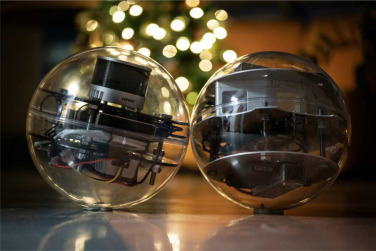
\includegraphics[width=0.5\textwidth]{pics/delta_kalman_robots.jpg}
    \label{fig:delta_kalman_robots}
    \caption{(Left:) A sphere platform featuring a 'Hesai Pandar-XT32'~\cite{Kalman_filter_sphere}. (Right:) A 'Livox Mid-100' Spherical platform from ~\cite{DeltaFilter}}
\end{figure}

While recent studies (e.g. \cite{Kalman_filter_sphere}) have compared their results with state-of-the-art SLAM systems such as DLIO~\cite{dlio} and FAST-LIO2~\cite{fastlio2}, the field continues to evolve rapidly. 
More recent SLAM algorithms (e.g., FAST-LIVO2~\cite{fastlivo2}), advanced LiDAR sensors like the MID-360 and RoboSense Airy, and modern single-board computers such as the Raspberry Pi 5 with PCIe support and Gigabit Ethernet are pushing the boundaries of what is possible. 
In this context, we introduce our first prototype, the non-actuated sphere, which leverages the processing power of the Raspberry Pi 5 16GB RAM model. 
This design enables real-time SLAM on a compact spherical platform, offering improved power efficiency, extended battery life, and reduced overall system cost.

\section{Spherical locomotion}\label{sec:sphere-locomotion}
Spherical locomotion has attracted significant research interest in recent years, driven by the pursuit of optimal mobility mechanisms. 
Although spherical robots may appear mechanically simple, a wide variety of locomotion strategies have been developed—and continue to emerge—requiring sophisticated control systems to manage the complex dynamics of rolling locomotion and internal mass distribution.

One of the most well-known approaches is the Internal Driving Unit (IDU), or differential drive, used in commercial robots like the Sphero Bolt+ and BB-8. 
Akella et al.~\cite{Sphero} analyzed BB-8’s internal wheel-driven system and demonstrated that effective control was achieved using only two actuators. 
However, they highlighted a key limitation: the robot’s geometry prevents controlled sliding and reduces effectiveness on inclined or uneven terrain.

In contrast, Zevering et al.~\cite{luna} introduced L.U.N.A., a spherical robot designed for autonomous 3D mapping in lunar caves. 
Rather than using wheels or rods, L.U.N.A. relies on internal flywheels to generate motion via the IBCOAM method. 
This approach enables a compact form factor and protects internal electronics, providing advantages particularly well suited to harsh and remote terrain. 
The robot demonstrated reliable motion on soft surfaces such as sand and rubber. 
However, limitations remain, including vibrational instability caused by unbalanced flywheels, reduced performance on inclined low-friction surfaces, and pose estimation errors due to unsynchronized sensor data.

In a following study, Zevering et al.~\cite{rod_sphere} proposed a rod-driven spherical robot, also targeting lunar cave exploration. 
This design uses external linear actuators to push against the environment to induce motion. 
While it improves adaptability to rugged terrain and sharp obstacles, it introduces new challenges, such as oscillatory behavior from fixed-speed actuators, limited effectiveness on slopes, and the need for higher-power actuation when traversing dusty or soft ground.

Beyond differential and flywheel-based designs, several researchers have explored pendulum-driven locomotion due to its mechanical simplicity, energy efficiency, and natural stability. 
Oevermann et al.~\cite{roboball}, Ren et al.~\cite{novelsphere}, and Kolbari et al.~\cite{pendulum_sphere} developed spherical robots that use an internal heavy pendulum as the primary driving mechanism. 
While their configurations differ in terms of shell design and target applications, they share a common reliance on pendulum-based locomotion and have demonstrated robust movement across a variety of terrains.
A notable example is RoboBall~\cite{roboball}, which features a novel soft pressurized shell and a two-degree-of-freedom internal pendulum. 
This robot successfully navigates gravel, grass, steep inclines, and even floats and maneuvers on water. 
However, the deformable shell introduces complex dynamic behavior. 
The researchers addressed this using a Linear Quadratic Regulator (LQR) for steering and a model-based proportional controller for driving. 
Ren et al.~\cite{novelsphere} experimented with both robust servo LQR (RSLQR) and PID-based stabilization strategies to enhance motion control and responsiveness, whereas Kolbari et al.~\cite{pendulum_sphere} adopted only PID control for stabilization. 

RoboBall’s experiments further revealed that internal pressure and shell deformation significantly affect dynamic behavior—especially due to the presence of a ``dead zone'' where balance control becomes unstable during motion.
Taken together, these pendulum-based locomotion strategies highlight the value of combining mechanical simplicity with robust control to enable adaptive movement in unpredictable environments.
While a variety of innovative locomotion methods have been proposed for spherical robots, including flywheel-, rod-, and pendulum-driven systems, few have been evaluated in conjunction with advanced LiDAR-inertial odometry algorithms under real-world motion dynamics, as briefly discussed in Section~\ref{AA}.
This thesis addresses this gap by introducing our second prototype, a pendulum-driven spherical robot designed to achieve both robust locomotion and accurate, real-time mapping performance within the constraints of a compact platform.

\chapter{Fundamentals and Theoretical Background}
\label{ch:fundamentals}
\section{Inertial Measurement Unit (IMU)}

An Inertial Measurement Unit (IMU) is an electronic device—either electromechanical or solid-state—that measures the specific force, angular rate, and, in some cases, the magnetic field of the object or body to which it is attached.
A 6-axis IMU typically employs accelerometers and gyroscopes, while a 9-axis IMU additionally incorporates a magnetometer. IMUs are widely used in aerospace, robotics, satellite navigation, and various other applications.

Micro-Electro-Mechanical Systems (MEMS) technology is commonly used in the production of IMUs. This technology enables the manufacturing of components that are extremely small and lightweight, with low power consumption, while also offering high reliability and cost efficiency~\cite{advnav_imu_intro,stanford_gps_lab_imu_testing}.
\subsection{Accelerometer}

\begin{figure}[ht]
\centering
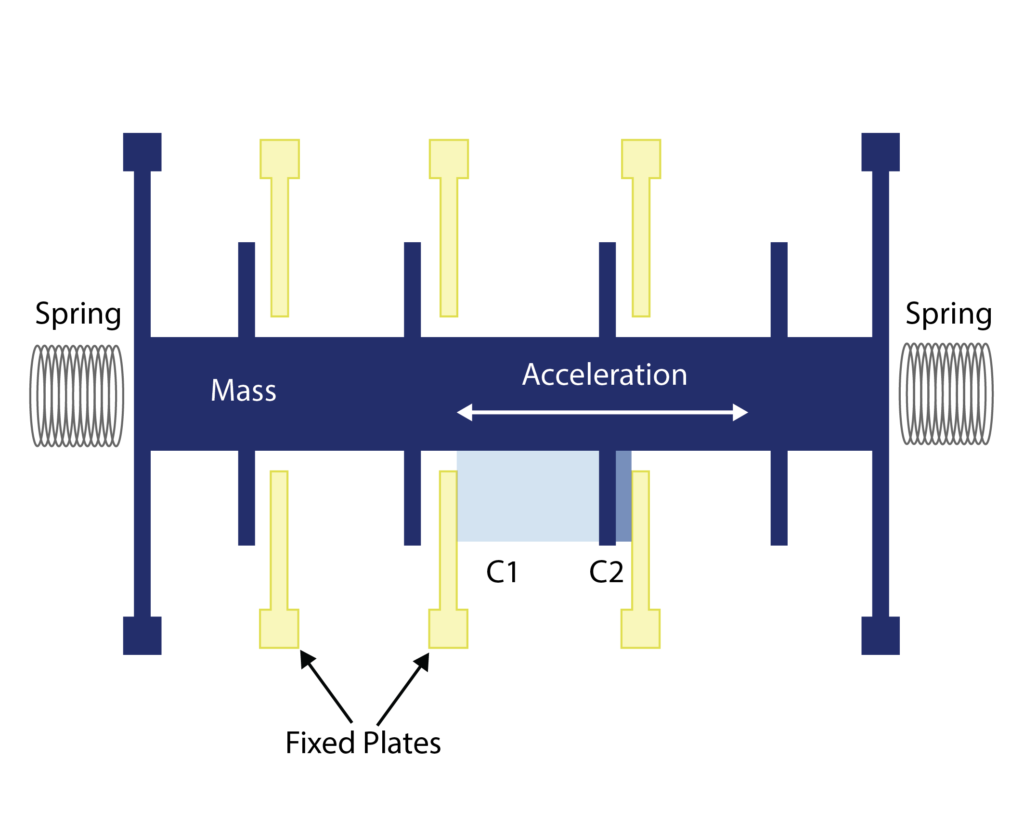
\includegraphics[width=\columnwidth]{pics/accel_inside.png}
\caption{Inside a MEMS accelerometer. The proof mass has fixed plates “fingers” between capacitor electrodes. At rest, they’re centered, giving zero acceleration. Movement during acceleration shifts the fingers, changing capacitance, which is used to calculate acceleration~\cite{ericco_mems_accel_vibrations}.}
\label{fig:inside_accel}
\end{figure}

An accelerometer in an IMU is a device that measures the linear acceleration of an object along the x, y, and z axes. From acceleration data, velocity and position can be derived by integrating the measured acceleration values over time. MEMS accelerometers measure the forces acting on them, which may arise from motion, gravity, or vibrations.

The accelerometer contains a proof mass connected to its frame via mechanical springs. These springs allow the proof mass to move along a direction known as the sensitivity axis. By monitoring the displacement of the proof mass from its original position, the accelerometer can determine the applied acceleration~\cite{ericco_mems_accel_vibrations}.

This displacement is typically measured using electrical capacitance. The device includes multiple differential capacitors, consisting of stationary electrodes positioned on either side of the proof mass, to accurately detect its movement, as illustrated in Fig.\ref{fig:inside_accel}.

\subsection{Gyroscope}

Gyroscopes are devices used to measure or maintain rotational motion.
The unit of angular velocity (a measure of how fast an object rotates) is typically expressed in degrees per second (°/s) or revolutions per second (RPS). 
Gyroscopes have a wide range of applications, including automotive rotation detection, inertial navigation, robotics, and motion tracking.

\begin{figure}[ht]
\centering
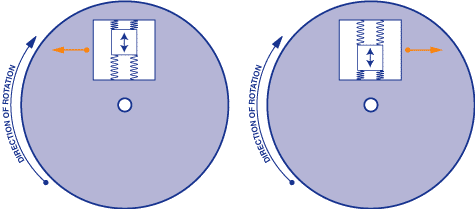
\includegraphics[width=\columnwidth]{pics/inside_gyro.png}
\caption{Inside a MEMS gyroscope. The small resonating mass shifts in response to angular velocity changes, generating electrical signals~\cite{sparkfun_gyroscope}.}
\label{fig:inside_gyro}
\end{figure}

A triple-axis MEMS (Micro-Electro-Mechanical Systems) gyroscope can measure rotation around three perpendicular axes: x, y, and z. The gyroscope sensor within a MEMS device is extremely small—typically between 1 and 100 micrometers, comparable to the thickness of a human hair. 
When the gyroscope is rotated, a small resonating mass inside the sensor shifts in response to changes in angular velocity. 
This movement generates minute electrical signals, which are then amplified and processed by a host microcontroller to determine the rotational motion~\cite{sparkfun_gyroscope,Pedestrian}.
\subsection{Magnetometer}

A \textit{magnetometer} is a sensor that measures the strength and direction of a magnetic field, most commonly the Earth's magnetic field.
In an IMU, magnetometers are primarily employed to estimate the heading, i.e., the orientation relative to magnetic north. 
This is achieved using a three-axis magnetometer, where three orthogonal sensing elements measure the magnetic field components along the $x$, $y$, and $z$ axes. 
From these measurements, the magnetic heading is computed and, when fused with gyroscope and accelerometer data, a north-referenced orientation can be obtained~\cite{advnav_imu_intro}.  

Several physical principles can be exploited in the construction of magnetometers, including fluxgate, anisotropic magnetoresistance (AMR), and giant magnetoresistance (GMR). 
For MEMS-based magnetometers, however, the \textit{Hall effect} is the most widely adopted mechanism. In this principle, a voltage difference is generated across a conductor when a magnetic field is applied perpendicular to the direction of current flow, allowing for direct measurement of magnetic field strength~\cite{howtomechatronics}.  

Despite their usefulness, magnetometers also present certain limitations. Their high sensitivity makes them susceptible to \textit{electromagnetic interference (EMI)} from nearby electronic devices as well as distortions caused by surrounding ferromagnetic materials. 
These disturbances, commonly referred to as \textit{soft-iron} and \textit{hard-iron} effects, can significantly reduce measurement accuracy. Consequently, proper calibration techniques, such as ellipsoid fitting or offset compensation, are necessary to ensure reliable heading estimation~\cite{vectornav_mems_operation}.

\section{LiDAR Technology}
Light Detection and Ranging (LiDAR) is a transformative sensing technology that enables accurate 3D perception of the environment. 
Unlike traditional cameras, which passively capture reflected light, LiDAR actively emits laser pulses and measures the time-of-flight of the returned signals. 
By repeating this process thousands of times per second, LiDAR builds dense point clouds that capture both the geometry and scale of the surrounding environment~\cite{neon_lidar_basics}.

Several LiDAR principles are commonly used:
\subsection*{Range-Finding LiDAR}
The most fundamental form, range finders, emit laser pulses and measure the time difference between emission and reception. 
This allows accurate distance measurements with high spatial resolution, particularly effective for small-scale targets due to the short laser wavelength compared to radar~\cite{bleier_advanced_sensory_systems}.  

\subsection*{Differential Absorption LiDAR (DIAL)}
DIAL systems measure atmospheric composition by exploiting the absorption characteristics of gases. 
Two laser beams are used: one at a wavelength corresponding to the absorption peak of a target gas (\textit{on-line}), and another at a nearby non-absorbing wavelength (\textit{off-line}). 
The ratio of the returned signals reveals the presence and concentration of the gas~\cite{bleier_advanced_sensory_systems}.  

\subsection*{Doppler LiDAR}
Doppler LiDAR utilizes the frequency shift (Doppler effect) of the returned signal to measure the velocity of moving particles such as aerosols. 
This technique is widely used for wind profiling, turbulence detection, and monitoring hazardous atmospheric conditions around launch sites~\cite{bleier_advanced_sensory_systems}.  

\subsection{Hybrid Solid-State LiDAR Technology}
Recent advancements in LiDAR move away from traditional mechanical spinning sensors toward solid-state and hybrid designs. 
These approaches reduce moving parts, improve robustness, and enable compact form factors suitable for mobile robots and drones. 
Instead of relying on repetitive scan lines, some hybrid LiDARs employ non-repetitive scanning patterns that gradually fill in the environment with dense coverage over time. 
This results in rich point clouds while maintaining lower cost and power consumption compared to high-end mechanical systems~\cite{globalgps_lidar_types,govcomm_compared}.  

An example of such technology is the \textbf{Livox Mid-360}, a hybrid solid-state LiDAR optimized for robotics and SLAM. 
It offers a full \(360^\circ\) horizontal field of view and employs a non-repetitive scanning pattern, making it highly effective for real-time mapping and obstacle avoidance in autonomous systems. Its balance of compact size, robustness, and dense perception capability makes it a suitable choice for research and mobile robotic applications~\cite{livox_mid360_docs}.

\section{Spherical Robot Types}
\label{sec:spherical-robot-types}
Spherical robots are well-known for their unique design compared to traditional wheeled or legged robots.
They have various ways to be designed for locomotion as described in Chapter~\ref{ch:state-of-the-art}.
In this section, we will describe the most common types of spherical robots based on their actuation mechanisms which can be broadly categorized into : \textbf{Barycentric} , \textbf{Conservation of Angular Momentum} and \textbf{rod-driven}.
\subsection{Barycentric}
Barycentric spherical robot depends on the displacement of the center of mass to achieve rolling motion.
This is achieved by using internal wheels or other mechanisms to shift the center of mass, allowing the sphere to roll in the desired direction~\cite{Aminata}.
\subsubsection{Hamester-driven}
One of the earliest form of Barycentric locomotion "hamster" design, as it mimics the movement of a hamster running inside a toy sphere. 
In this concept, a small wheeled robot is placed within the shell, and its weight and motion generate the force needed to roll the structure. Different internal vehicles can be used, such as single- or multi-wheeled robots, with four-wheel differential-drive systems offering additional maneuverability and even the ability to turn in place. 
The design is relatively simple to build and operate, but challenges arise from wheel slippage, friction losses, and instability when the internal robot becomes airborne over uneven surfaces. 
These issues can lead to loss of traction, reduced momentum, and tracking errors, limiting its effectiveness for tasks requiring precise navigation~\cite{flywheel_hamaster_explanation}.

\subsubsection{Spring-loaded locomotion}
In this design, a spring–rod mechanism is mounted on the top of the internal robot and pressed against the inner surface of the spherical shell. 
The spring ensures that the robot’s driving wheels remain in continuous contact with the shell, providing stable traction and controlled motion. 
To minimize friction at the contact point, a three-degree-of-freedom (DOF) ball bearing is integrated at the end of the spring. 
This bearing allows smooth sliding along the inner shell surface while accommodating multi-directional movement, thus improving efficiency, reducing energy loss, and enhancing overall maneuverability within the spherical structure~\cite{old_spring_paper,flywheel_hamaster_explanation,SpheriDrive}.


\begin{figure}[ht]
    \centering
\begin{subfigure}{0.48\textwidth}
    \centering
    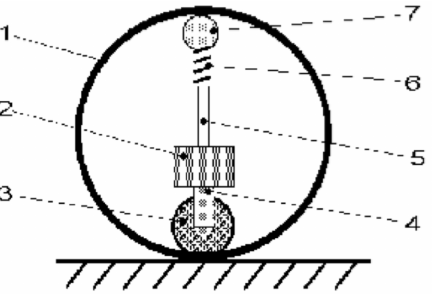
\includegraphics[width=0.9\textwidth]{pics/spring_2d.png}
    \caption{Structure of (Spring-loaded) Robot. 1. robot body (case), 2. controlling box, 3. driving wheel, 4. steering axis, 5. supporting axis, 6. spring, 7. balance wheel~\cite{old_spring_paper}}
    \label{fig:spring_2D_top}
\end{subfigure}

\begin{subfigure}{0.48\textwidth}
    \centering
    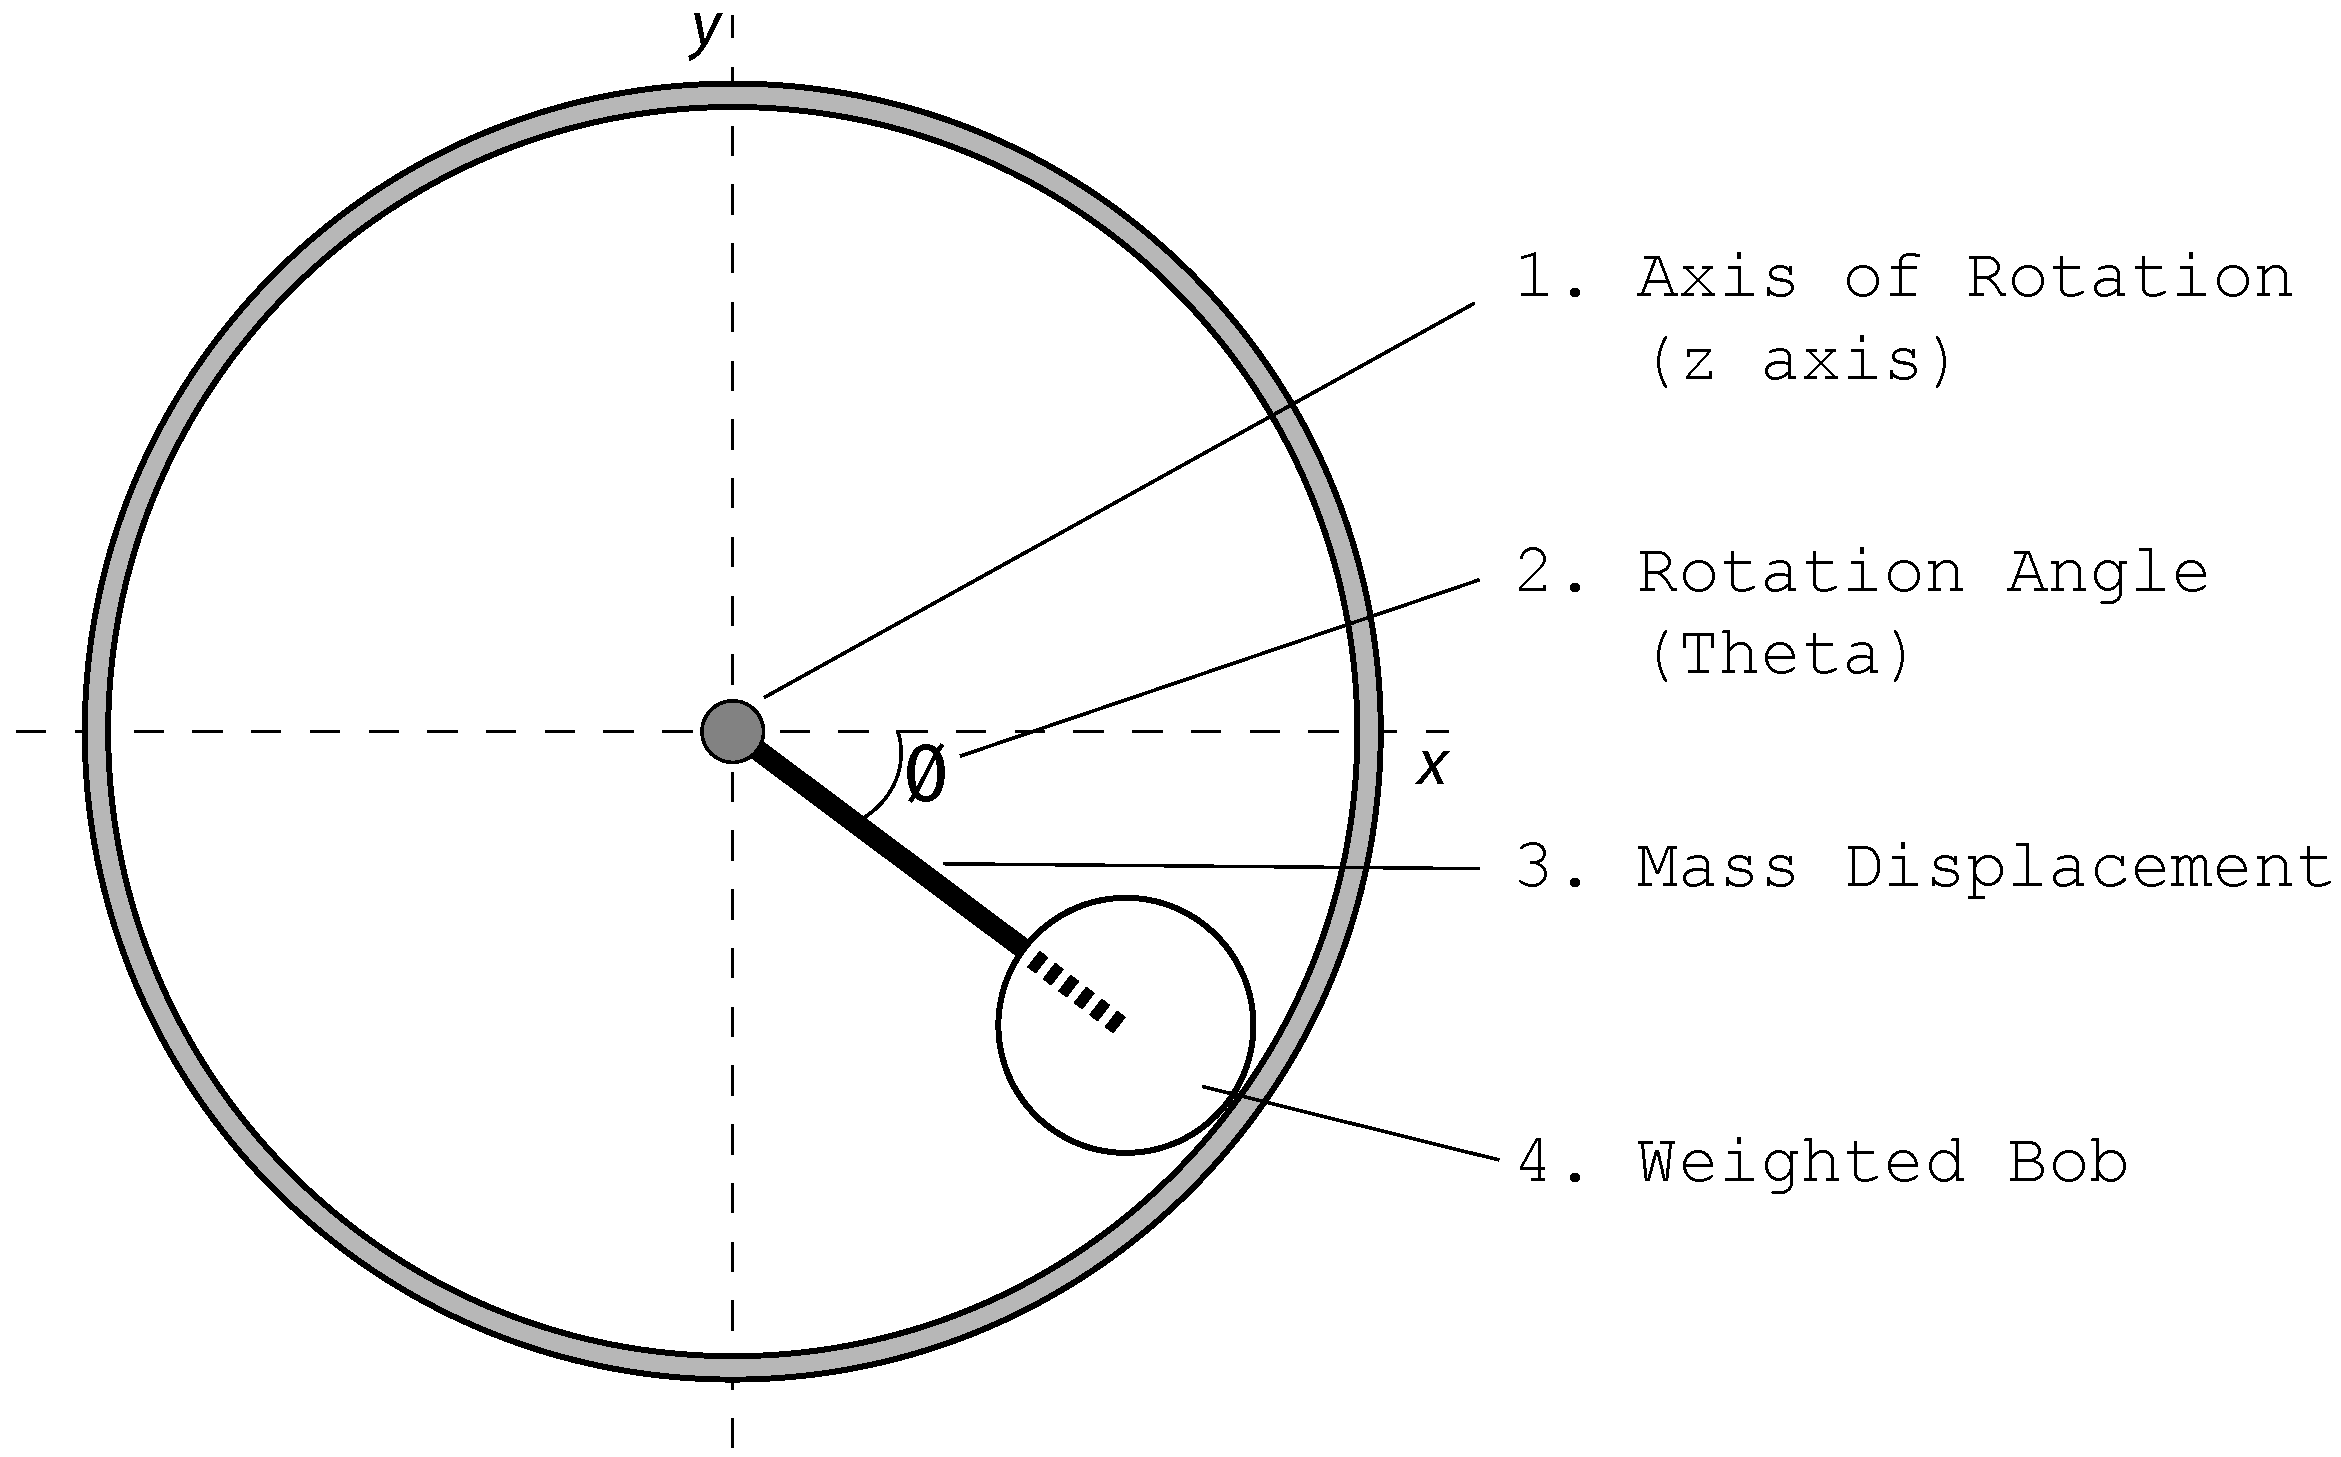
\includegraphics[width=0.9\textwidth]{pics/pendulum_mechanism.png}
    \caption{Structure of (Pendulum-driven) Robot.}
    \label{fig:pendulum_2D}
\end{subfigure}


\caption{Various spherical robot actuation mechanisms.}
\label{fig:spring_sphere}
\end{figure}



\subsubsection{pendulum-driven mechanism}
A pendulum-driven spherical robot is a type of \textit{barycentric sphere robot} that relies on shifting its internal center of mass for locomotion. 
The robot consists of a spherical shell, a central shaft, an internal pendulum, and typically two motors (or a dual-axis torque motor), as illustrated in Fig.~\ref{fig:pendulum_2D}. 
The pendulum, mounted near the inner surface of the shell, is connected to the center of the sphere and actuated by a motor or high-precision servo. 
By swinging the pendulum to the left or right, the robot shifts its center of mass, causing the shell to roll laterally. 
Meanwhile, the dual-axis torque motor controls forward and backward motion by controlling the pendulum’s orientation. 
This design provides a relatively simple and energy-efficient method of achieving mobility, though its torque is limited by the pendulum’s displacement and gravitational force~\cite{pendulum_sphere,Pendulum_Driven_Spherical_Robot,roboball}.


\subsection{Conservation of Angular Momentum}
Instead of moving the center of mass for the rolling motion, the motion of this sphere is achieved by using reaction wheel. 
We will focus on the flywheel-driven mechanism, which is a specific implementation of the conservation of angular momentum principle~\cite{Aminata}.
\subsubsection{Flywheel-driven}
The flywheel mechanism in spherical robots operates on the principle of conservation of angular momentum (COAM), where a rapidly spinning internal rotor generates torque to drive motion. By accelerating, decelerating, or reorienting the flywheel, reaction torques are imparted to the spherical shell, enabling controlled movement.
More advanced implementations use Control Moment Gyroscopes (CMGs), in which a high-speed flywheel mounted on a gimbal produces torque in an orthogonal axis when rotated, thus amplifying output power.
One of examples that follow this mecahnism is L.U.N.A~\cite{luna} via the Impulse by Conservation of Angular Momentum (IBCOAM) method.
Compared to barycenter-offset systems, flywheel-based designs are not limited by the internal center of mass and can achieve higher torques, improved agility, and even holonomic motion with multi-axis configurations.
However, these systems introduce challenges such as precession-induced instability, nonlinear dynamics, and high energy demands, requiring sophisticated control strategies for stable and precise operation~\cite{flywheel_hamaster_explanation}.
\begin{figure}[ht]
    \centering
    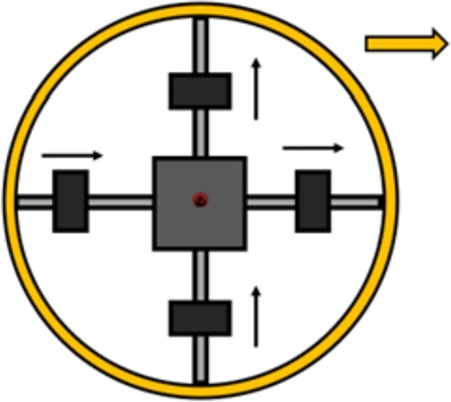
\includegraphics[width=0.3\textwidth]{pics/flywheel_2D_top.jpg}
    \label{fig:flywheel_2D_top}
    \caption{Flywheel-based simplified 2D top view of one example of flywheel mechanism, where the flywheel's angular momentum is used to generate torque for movement~\cite{SpheriDrive}.}
\end{figure}

\subsection{Rod-Driven Mechanism}
The rod-driven mechanism for spherical robots generates locomotion by extending and retracting internal rods positioned within the sphere. 
There are two primary ways in which these rods can initiate rotation. 
The first is the \textit{pushing approach}, where rods on the side opposite to the intended rolling direction extend outward to make contact with the ground. 
By exerting force against the surface, they generate a reaction torque that propels the sphere in the desired direction. 
The second method is the \textit{leverage approach}, in which the weight of the rods themselves is used to shift the robot’s center of mass. 
When extended without contacting the ground, the displaced weight creates torque that induces rotation. 
In practice, a combination of pushing and leverage is often employed, where the rods provide both active ground interaction and passive weight shifting, resulting in more efficient and controllable locomotion. 
However, experiments have shown several challenges: on soft or sandy surfaces the mechanism struggles to generate enough torque due to actuator limitations, while on solid ground poorly chosen extension angles can lead to unstable or oscillatory motion. 
Moreover, leverage alone often fails to move the robot effectively, and even combined push-and-leverage control may cause stalling or uncontrolled rolling, requiring manual intervention~\cite{rod_sphere}.



\section{Introduction to SLAM}
Simultaneous Localization and Mapping (SLAM) addresses the problem of enabling a robot to navigate in an unknown environment while building a consistent map of that environment.
A robot typically starts at an initial position and moves through an environment with uncertain motion dynamics. 
Over time, this uncertainty grows, making it increasingly difficult for the robot to accurately estimate its pose in global coordinates. 

To overcome this challenge, the robot relies on its onboard sensors---such as cameras, LiDAR, radar, and IMU---which are inherently affected by noise. 
Using these noisy measurements, the robot incrementally builds a representation of the environment (a map) while simultaneously estimating its position relative to that map in real time~\cite{slam_problem}. 

Researchers have developed a variety of SLAM algorithms to address this problem with improved accuracy, robustness, and computational efficiency.
Among the widely studied methods are \textit{Visual-Inertial Odometry (VIO)}, \textit{LiDAR-Inertial Odometry (LIO)}, and their hybrid variant \textit{LiDAR-Inertial-Visual Odometry (LIVO)}. 
These approaches form the foundation of many modern SLAM systems.
\subsection{Visual-Inertial Odometry (VIO)}
VIO fuses visual data (from monocular, stereo, or RGB-D cameras) with inertial data from an IMU. 
The visual input provides rich environmental features, while the IMU provides high-frequency motion estimates~\cite{inertiallabs_vio_revolution,Survey_odometry}.

Some of its advantages include:
\begin{itemize}
    \item Works well in texture-rich environments.
    \item IMU compensates for fast motions and reduces scale ambiguity in monocular systems.
    \item More lightweight than LiDAR-based methods.
\end{itemize}

However, VIO also has some limitations:
\begin{itemize}
    \item Struggles in low-light or feature-poor environments.
    \item Sensitive to camera calibration and rolling-shutter effects.
    \item Drift can accumulate without loop closure.
\end{itemize}

\subsection{LiDAR-Inertial Odometry (LIO)}
LIO integrates LiDAR scans with IMU measurements. LiDAR provides highly accurate geometric information about the surroundings, while the IMU contributes motion constraints.
By combining these two sources of information, LIO can estimate the robot's pose more accurately and robustly, even in challenging environments~\cite{lee2024_lidar_odometry_survey,fastlio2}.

Some of its advantages include:
\begin{itemize}
    \item Good performance in environments with poor lighting or visual features.
    \item Provides accurate 3D geometry and range data.
    \item Less sensitive to environmental changes compared to vision-based methods.
\end{itemize}

However, LIO also has some limitations:
\begin{itemize}
    \item LiDAR sensors are expensive and power-hungry.
    \item Struggles in featureless areas (e.g., tunnels with uniform walls).
    \item Lower spatial resolution compared to cameras.
\end{itemize}

\subsection{LiDAR-Inertial-Visual Odometry (LIVO)}
LIVO combines the strengths from VIO and LIO by integrating data from both vision and LiDAR, together with IMU.
Visual features improve robustness in environments where LiDAR degeneracy occurs, while LiDAR provides reliable geometry where vision fails (e.g., in poor lighting)~\cite{yuan2024sr,fastlivo2}.

Some of its advantages include:
\begin{itemize}
    \item Strong robustness by exploiting complementary sensor modalities.
    \item Reduced degeneracy problems (both visual and LiDAR weaknesses are compensated).
    \item Often achieves state-of-the-art accuracy in SLAM benchmarks.
\end{itemize}

However, LIVO also has some limitations:
\begin{itemize}
    \item High computational complexity and sensor fusion challenges.
    \item Requires precise extrinsic calibration among LiDAR, camera, and IMU.
    \item Higher hardware cost and system integration complexity.
\end{itemize}

\section{Control Strategies}
\label{sec:control-strategies}
Control strategies play a crucial role in various robotic applications and spherical robots are no exception.
These strategies are essential for achieving precise motion control, stability, and adaptability to dynamic environments.
There are two types of control strategies: open-loop and closed-loop control.
An \textbf{open-loop system} relies solely on the system's model, without input from past performance or supporting measurements. In contrast, a \textbf{closed-loop system} uses feedback---such as errors or results from previous operations---to continuously adjust and improve its performance. Fig. \ref{fig:control_systems} illustrates the difference between the two systems~\cite{feedbackBook,vectornav_math_controls}.

\begin{figure}[ht]
\centering
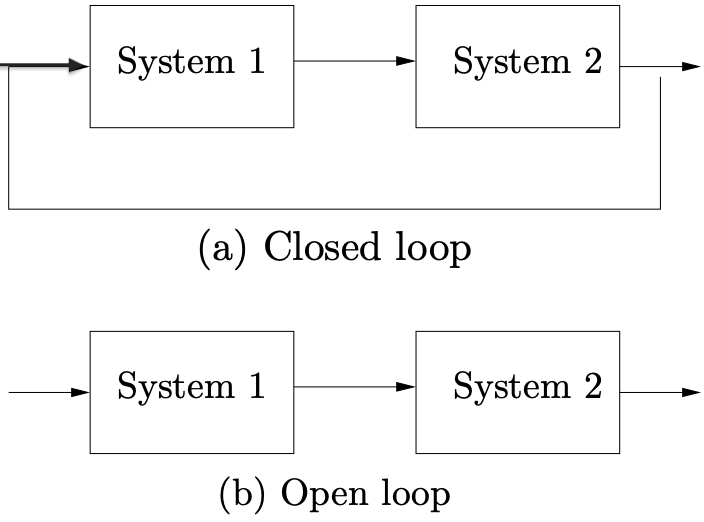
\includegraphics[width=0.4\columnwidth]{pics/systems.png}
\caption{Comparison of closed-loop and open-loop control systems~\cite{feedbackBook}.}
\label{fig:control_systems}
\end{figure}

In this section, we will discuss two widely used control strategies: Proportional-Integral-Derivative (PID) control and Linear Quadratic Regulator (LQR) control.
These methods are particularly relevant for spherical robots, where maintaining balance and achieving accurate movement is critical since they are designed to roll in all directions.
\subsection{PID Control}
Proportional–integral–derivative (PID) control is one of the most widely used methods of implementing feedback (closed-loop systems) in applications ranging from industrial processes and manufacturing to simple balancing robots~\cite{feedbackBook}. 
A PID controller combines three types of control actions: proportional, integral, and derivative. The feedback correction term is obtained by applying individual gain values to each of these control components, as illustrated in Figure~\ref{fig:pid_control}.
\begin{figure}[ht]
\centering
\includegraphics[width=0.7\columnwidth]{pics/pid_control.png}
\caption{PID Controller Block Diagram~\cite{vectornav_math_controls}.}
\label{fig:pid_control}
\end{figure}

Considerable research has been devoted to determining the optimal gain values for these terms across a broad spectrum of systems.

\textbf{Proportional Control (P):}  
The proportional term applies a gain factor $K_p$ to the instantaneous error $e(t)$, which is defined as the difference between the desired state and the measured state:
\begin{equation}
    u_P(t) = K_p e(t)
    \label{eq:P}
\end{equation}
Proportional control is the simplest form of feedback control to implement. However, when used alone, it generally results in a steady-state error in the system.

\textbf{Integral Control (I):}  
The integral term accumulates the error over time and scales it by a gain factor $K_i$:
\begin{equation}
    u_I(t) = K_i \int_{0}^{t} e(\tau) \, d\tau
    \label{eq:I}
\end{equation}
When combined with proportional control, the integral component effectively acts as a low-pass filter, compensating for steady-state errors. Nevertheless, excessive integration can lead to integral windup, causing the system to overshoot the target value.

\textbf{Derivative Control (D):}  
The derivative term acts on the rate of change of the error and is multiplied by a gain factor $K_d$:
\begin{equation}
    u_D(t) = K_d \frac{de(t)}{dt}
    \label{eq:D}
\end{equation}
This allows the controller to anticipate future error trends. The faster the error changes, the stronger the influence of the derivative term. When tuned appropriately, derivative control helps prevent overshoot and enhances system stability.

\textbf{Combined PID Control:}  
The total control input is obtained by summing the three components:
\begin{equation}
    u(t) = u_P(t) + u_I(t) + u_D(t) 
         = K_p e(t) + K_i \int_{0}^{t} e(\tau)\, d\tau + K_d \frac{de(t)}{dt}
    \label{eq:PID}
\end{equation}
This combined feedback correction term is applied to the system input—commonly referred to as the plant—to drive the dynamics toward the desired state. The gain values $K_p$, $K_i$, and $K_d$ can be tuned to achieve the desired system response. In practice, this tuning is typically performed through iterative testing and experimentation. When implemented on digital controllers or microcontrollers, the same principles apply, but the PID algorithm must be expressed in discrete form to account for fixed sampling intervals and computational constraints, as shown in Eq.~\ref{eq:pid_control}~\cite{vectornav_math_controls,PIDBook2}.

\textbf{Discrete PID Control:}  
While the continuous-time formulation of PID control (Eq.~\ref{eq:PID}) provides the theoretical basis, most real-world applications rely on a discrete implementation, since digital controllers operate with fixed sampling intervals. The discrete form of the PID controller is given by

\begin{equation}
u[k] = K_p \cdot e[k] + K_i \cdot \sum_{i=0}^{k} e[i] \cdot \Delta t + K_d \cdot \frac{e[k] - e[k-1]}{\Delta t}
\label{eq:pid_control}
\end{equation}

where $u[k]$ represents the control signal (e.g., the servo motor command) at the $k$-th time step, $e[k]$ is the error between the target angle $\theta_{\text{target}}$ and the current angle $\theta_{\text{current}}$, and $K_p$, $K_i$, $K_d$ are the proportional, integral, and derivative gains, respectively. The controller operates at a fixed sampling period $\Delta t$, which replaces the continuous integral and derivative operations with their discrete equivalents.

In practice, the discrete controller enables real-time implementation on microcontrollers and embedded systems. Enhancements such as introducing a deadband around the setpoint can suppress small oscillations, while resetting the integral term within this region helps prevent windup. Moreover, manual control inputs may be superimposed on the PID output, and the resulting command is constrained within actuator limits to ensure safe and stable operation. Compared to the continuous formulation, the discrete PID explicitly accounts for sampling and computational constraints, making it more suitable for digital hardware implementations

\subsection{Linear Quadratic Regulator (LQR)}

The \textit{Linear Quadratic Regulator} (LQR) is considered one of optimal control theory, particularly notable for its analytical tractability in stabilizing linear time-invariant systems with a quadratic cost functional. For a system modeled in state-space form as
\[
\dot{\mathbf{x}} = \mathbf{A} \mathbf{x} + \mathbf{B} \mathbf{u},
\]
the infinite-horizon cost to be minimized is taken as
\[
J = \int_{0}^{\infty} \left( \mathbf{x}^{T} \mathbf{Q} \, \mathbf{x} + \mathbf{u}^{T} \mathbf{R} \, \mathbf{u} \right) \, dt,
\]
where \(\mathbf{Q} = \mathbf{Q}^{T} \succeq 0\) and \(\mathbf{R} = \mathbf{R}^{T} \succ 0\) are the state and control weight matrices~\cite{underactuatedLQR}.

By assuming the optimal cost-to-go function \(J^*(\mathbf{x})\) is quadratic, \(J^*(\mathbf{x}) = \mathbf{x}^T \mathbf{S} \mathbf{x}\), and substituting this into the Hamilton–Jacobi–Bellman condition, one derives an algebraic Riccati equation:
\[
\mathbf{A}^T \mathbf{S} + \mathbf{S} \mathbf{A} - \mathbf{S} \mathbf{B} \mathbf{R}^{-1} \mathbf{B}^T \mathbf{S} + \mathbf{Q} = \mathbf{0}.
\]
The solution \(\mathbf{S}\) subsequently yields the optimal state-feedback law
\[
\mathbf{u}^*(\mathbf{x}) = -\mathbf{R}^{-1} \mathbf{B}^T \mathbf{S} \, \mathbf{x} = -\mathbf{K} \mathbf{x},
\]
where \(\mathbf{K} = \mathbf{R}^{-1} \mathbf{B}^T \mathbf{S}\) is the gain matrix~\cite{underactuatedLQR}.

LQR's appeal lies in its closed-form solution, robustness guarantees, and minimal reliance on computational resources, making it especially valuable as a baseline controller in robotic systems. Recent studies have shown that actuated spherical robots increasingly adopt LQR-based control rather than classical PID approaches, since LQR can explicitly handle multi-variable state coupling and achieve smoother stabilization. This research highlights LQR’s suitability for nonlinear robotic platforms where traditional PID controllers face some limitations~\cite{novelsphere}.



\chapter{Hardware Design}
\label{ch:hardwaredesign}

This chapter describes the hardware design and structural implementation of two spherical robots developed for 3D mapping: the non-actuated sphere and the actuated sphere.

\section{Non-Actuated Sphere}
\subsection{Design Considerations}

The non-actuated sphere was modeled using CAD software, drawing inspiration from the design by Arzberger et al.~\cite{Kalman_filter_sphere}.
Its structure features two flat discs stacked vertically and secured with pillar screws, leaving a gap of approximately \SI{28}{\milli\meter} between them for internal components. 

The diameter of the discs was calculated using the Pythagorean theorem~\ref{Pythagorean} to ensure proper spacing for adding all internal components needed.
\begin{equation}
    R = \sqrt{h^2 + r^2} \label{Pythagorean}
\end{equation}


\noindent
where $R$ is the disc radius, $h$ is half the vertical spacing between the discs, and $d$ is the radius of the disc.

To enhance structural integrity and safety, fillets were applied to the edges of the discs. 
Each disc has a uniform thickness of \SI{3}{\milli\meter}.
The overall external diameter of the sphere is \SI{16}{\centi\meter}, making it compact and lightweight (less than \SI{1}{\kilo\gram}, including battery and electronics).
A key requirement was achieving stable and predictable rolling behavior. 
To this end, the center of mass was aligned with the geometric center of the sphere by strategically placing small metal weights. 
This alignment prevented wobbling and ensured smooth motion when the sphere was manually pushed by hand or foot.

\subsection{Fabrication Methods}
Two fabrication approaches were explored for the discs:
\begin{itemize}
    \item \textbf{3D Printing with PLA,} which enabled rapid prototyping and iterative testing.
    \item \textbf{Laser Cutting with Acrylic,} which provided greater rigidity.
\end{itemize}
Both materials demonstrated sufficient durability during initial testing.

\subsection{Component Integration}
The internal layout of the non-actuated sphere was divided into three layers (Table~\ref{tab:hardware_components_non_actuated}).
Components were arranged to balance weight distribution and minimize cable routing complexity.

\begin{figure}
\centering
\begin{subfigure}{0.4\columnwidth}
    \centering
    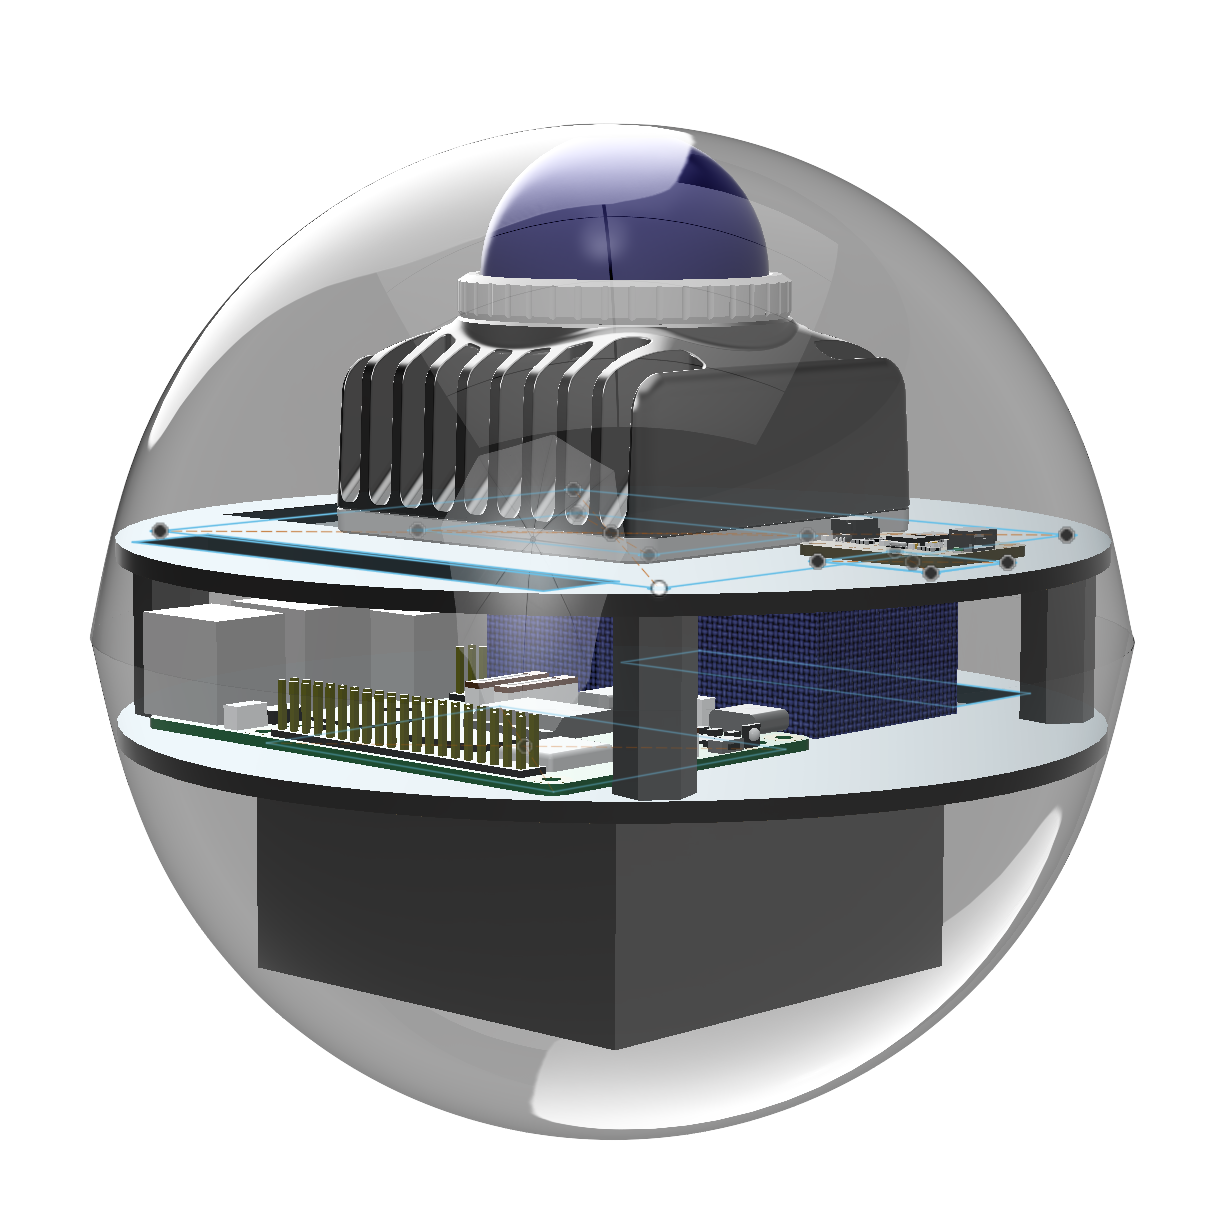
\includegraphics[width=\textwidth]{pics/Non_actuated_Sphere_CAD.png}
    \caption{3D CAD model}
    \label{fig:cad-model}
\end{subfigure}
\hfill
\begin{subfigure}{0.4\columnwidth}
    \centering
    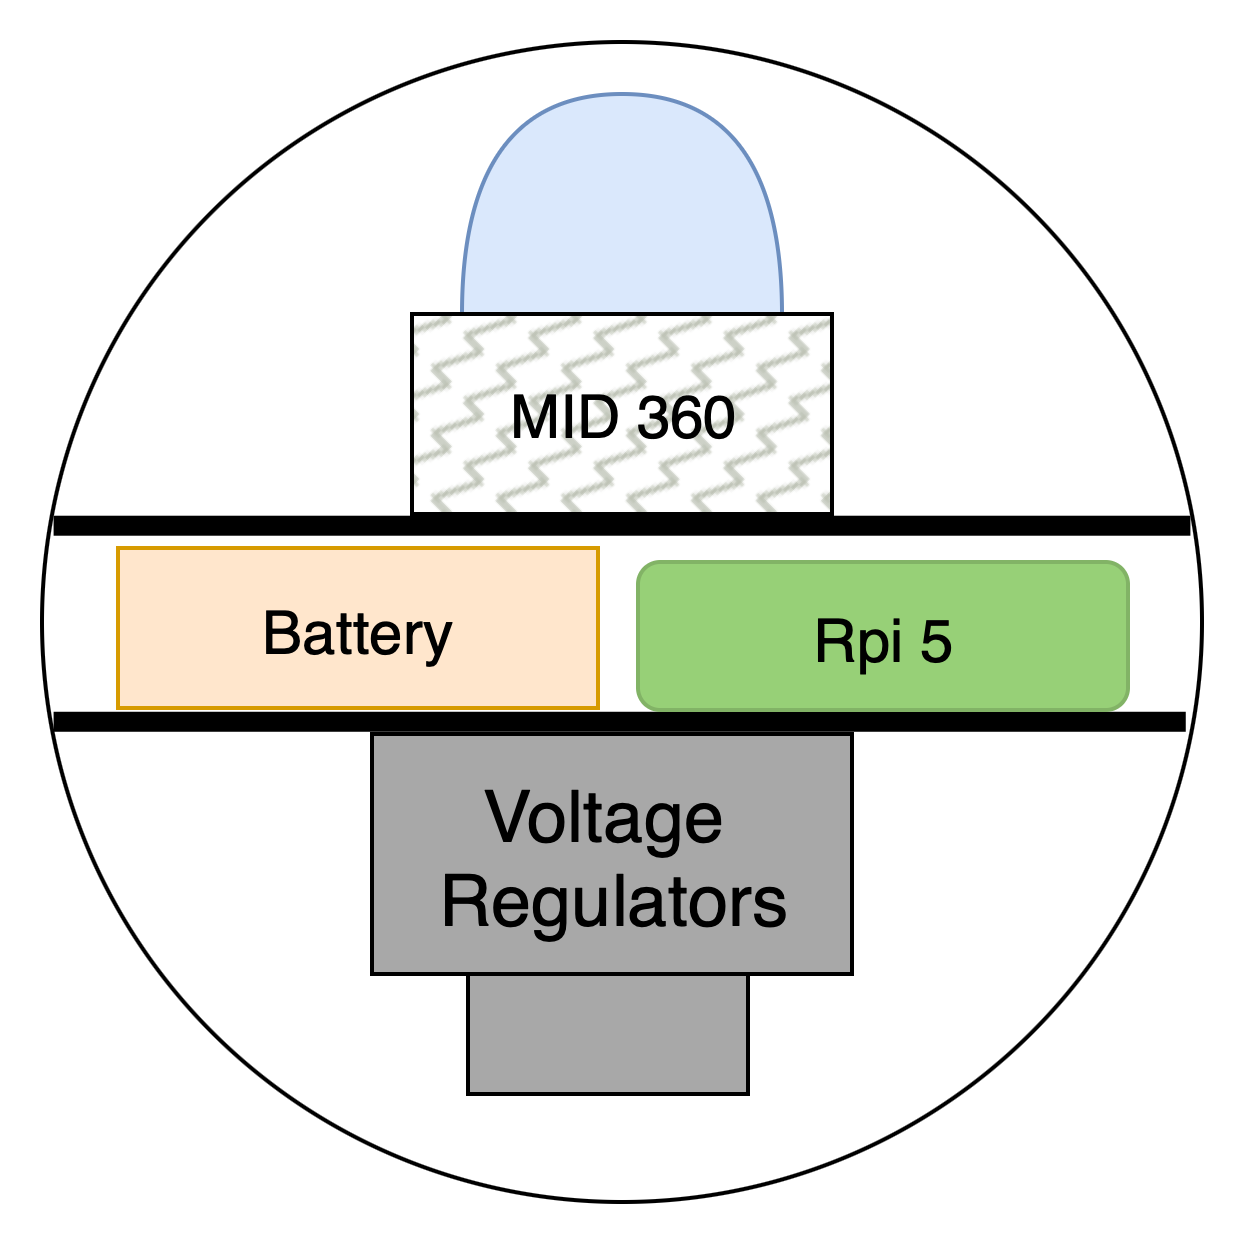
\includegraphics[width=\textwidth]{pics/image.png}
    \caption{Simplified 2D Model}
    \label{fig:2d-model}
\end{subfigure}
\caption{Schematic model and design of the non-actuated sphere.
It must be pushed manually.}
%\vspace{-4mm}
\label{fig:cad-design1}
\end{figure}
\begin{table}
\centering
\caption{Hardware components and placement in non-actuated sphere}
\label{tab:hardware_components_non_actuated}
\begin{tabularx}{\linewidth}{@{}l X@{}}
\toprule
\textbf{Layer} & \textbf{Components} \\
\midrule
Top    & Livox Mid-360 LiDAR, BNO-085 IMU \\
Middle & Raspberry Pi 5 (16 GB, 256 GB SSD, cooling fan) \\
       & 2200 mAh 3S LiPo battery \\
Bottom & 12V 10A voltage regulator \\
       & 5V 5A voltage regulator (for Raspberry Pi 5) \\

\bottomrule
\end{tabularx}
\vspace{-1em}
\end{table}
Table~\ref{tab:hardware_components_non_actuated} summarizes the components used in the non-actuated sphere and their locations within the sphere.
Each component was carefully selected to ensure its compatibility with the sphere's design and operational requirements:
\begin{itemize}
    \item \textbf{Livox Mid-360 LiDAR:} was mounted on the top layer to maintain an unobstructed 360° field of view.
    \item \textbf{Raspberry Pi 5:} was placed in the middle layer, providing sufficient processing power for real-time SLAM.
    \item \textbf{LiPo Battery:} a 2200 mAh 3S battery was used to power the system, ensuring a balance between weight and runtime.
    \item \textbf{Voltage Regulators:} a 12V 10A voltage regulator was used to power the LiDAR, while a 5V 5A regulator powered the Raspberry Pi 5.
\end{itemize}
The Livox Mid-360 is connected to the Raspberry Pi via Ethernet, while the BNO-085 IMU communicates through the I2C interface. 
A 3D CAD model of the assembled structure is shown in Fig.~\ref{fig:cad-design1}.
Simple 2D Drawings of the sphere with dimensions are shown in Fig.~\ref{fig:2d-model}.

The complete structural design of the non-actuated sphere is shown in section~\ref{sec:complete-structure}.
For reproducibility, the complete CAD and 2D design files are made openly available in our GitHub repository~\cite{githubsphere} and Section~\ref{sec:non-actuated-sphere-drawings}.
\clearpage


\begin{figure}[ht]
\begin{subfigure}{0.47\columnwidth}
    \centering
    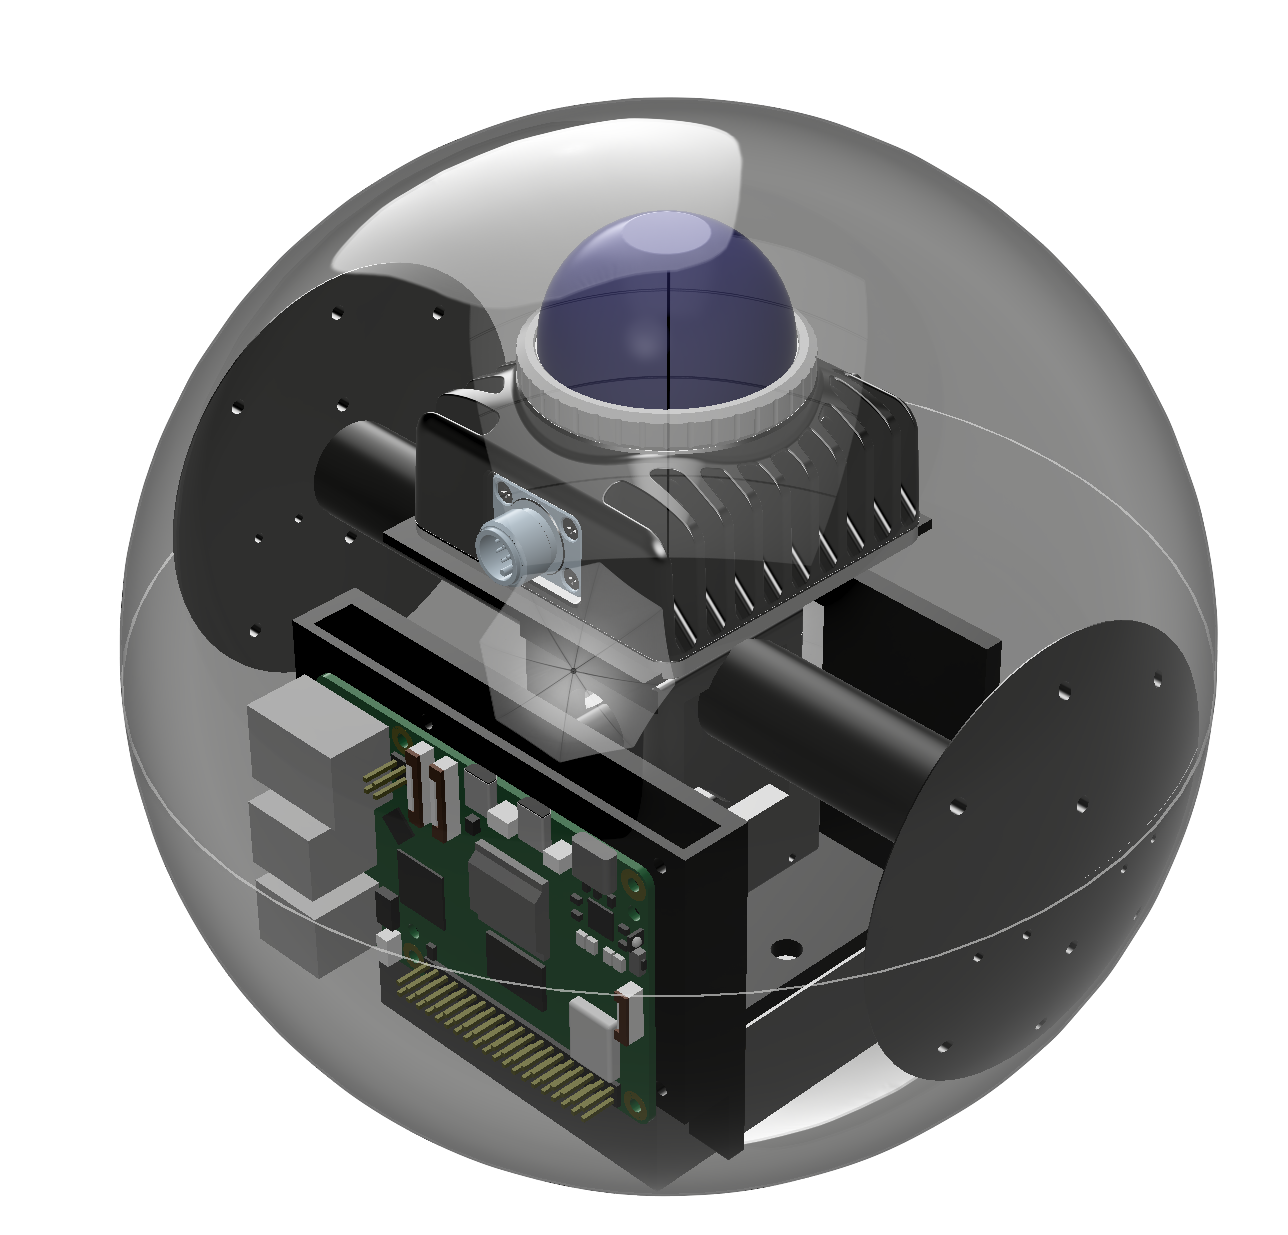
\includegraphics[width=\textwidth]{pics/Actuated_sphere.png}
    \caption{3D CAD model}
    \label{fig:cad-design2}
\end{subfigure}
\hfill
\begin{subfigure}{0.52\columnwidth}
    \centering
    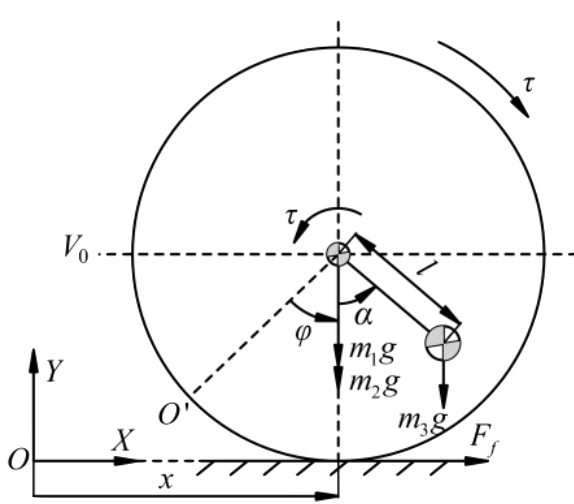
\includegraphics[width=\textwidth]{pics/planer_model.png}
    \caption{Pendulum model~\cite{Sphere_2D}}
    \label{fig:2d-model2}
\end{subfigure}
\caption{Schematic model and design of the actuated sphere.
The sphere uses a servo motor for actuation through pendulum-driven locomotion.
A second servo shifts the center of mass laterally by moving the battery to enable curved trajectories.}
\label{fig:act-cad-design2}
\end{figure}
\section{Actuated Sphere}
\subsection{Design Considerations}
The actuated sphere was designed using CAD software, with its final structure illustrated in Fig.~\ref{fig:act-cad-design2}. As described in Section~\ref{sec:sphere-locomotion}, the design was inspired by pendulum-driven locomotion mechanisms reported in related works~\cite{roboball, novelsphere}.  

Unlike the non-actuated sphere, this version have an internal actuation system that enables autonomous locomotion.
At its core, a \textbf{Waveshare Smart Continuous Servo (ST3215)} provides forward and backward motion by dynamically shifting the internal center of mass. 
A second \textbf{PWM-controlled servo} produces lateral displacement of the pendulum, enabling left and right turns.  



The simplified dynamic model of the robot, shown in Fig.~\ref{fig:2d-model2}, captures the essential motion parameters:  
\begin{itemize}
    \item robot horizontal position \( x \),  
    \item shell rotation angle \( \phi \),  
    \item pendulum swing angle \( \alpha \),  
    \item applied motor torque \( \tau \).  
\end{itemize}

The physical properties considered in the design include:  
\begin{itemize}
    \item shell mass \( m_1 \),  
    \item driver mass \( m_2 \),  
    \item counterweight mass \( m_3 \),  
    \item gravitational acceleration \( g \),  
    \item pendulum rod length \( l \).  
\end{itemize}

These parameters guided the selection of servo specifications and overall component placement to balance actuation efficiency with structural stability.  

\subsection{Fabrication Method}
The structural components were fabricated from \textbf{PLA filament}, produced by 3D printing in multiple sections and assembled into the final spherical form. PLA was selected for this prototype due to its light weight, ease of fabrication, and sufficient strength for housing the actuation system.  

\subsection{Component Integration}
The internal components were distributed across specific positions within the sphere, as summarized in Table~\ref{tab:hardware_components_actuated}. Placement was chosen to maximize balance and minimize unnecessary torque on the servos:  

\begin{itemize}
    \item The \textbf{primary servo motor} was centrally mounted, ensuring stable pendulum motion.  
    \item The \textbf{PWM servo} was aligned laterally to allow controlled sideward displacement.  
    \item The \textbf{LiPo battery} was placed at the rear.
    \item The \textbf{counterweight} was positioned at the front to balance the mass of the battery.
    \item Voltage regulators were distributed between the pendulum module and rear compartment to reduce thermal buildup and electrical noise.  
    \item Sensors were mounted on the top for clear environmental perception (LiDAR and Pi Camera).  
\end{itemize}

The detailed CAD drawings of the actuated sphere are presented in Section~\ref{sec:actuated-sphere-drawings}.
These include orthographic projections, component placement, and disc dimensions, providing a complete overview of the mechanical layout.  


\begin{table}
\centering
\caption{Hardware components and placement in the actuated sphere}
\label{tab:hardware_components_actuated}
\begin{tabularx}{\linewidth}{@{}l X@{}}
\toprule
\textbf{Position} & \textbf{Components} \\
\midrule
Center & Waveshare Smart Continuous Servo (model ST3215) \\
       & Forward/backward actuation \\
       & PWM Servo – left/right pendulum control \\
Rear   & 2200 mAh 3S LiPo battery \\
       & 5V 5A voltage regulator (for Raspberry Pi 5) \\
       & 6V UBEC (for servo motors) \\
Pendulum Module & 12V 20A voltage regulator – powers the entire system; positioned near the shell for stability \\
Front  & Raspberry Pi 5 (16 GB model) \\
Top    & Livox Mid-360 LiDAR \\
       & Pi Camera V3 (12 MP) \\
\bottomrule
\end{tabularx}
\vspace{-4mm}
\end{table}



\chapter{Software Design}

\begin{figure*}
    \centering
    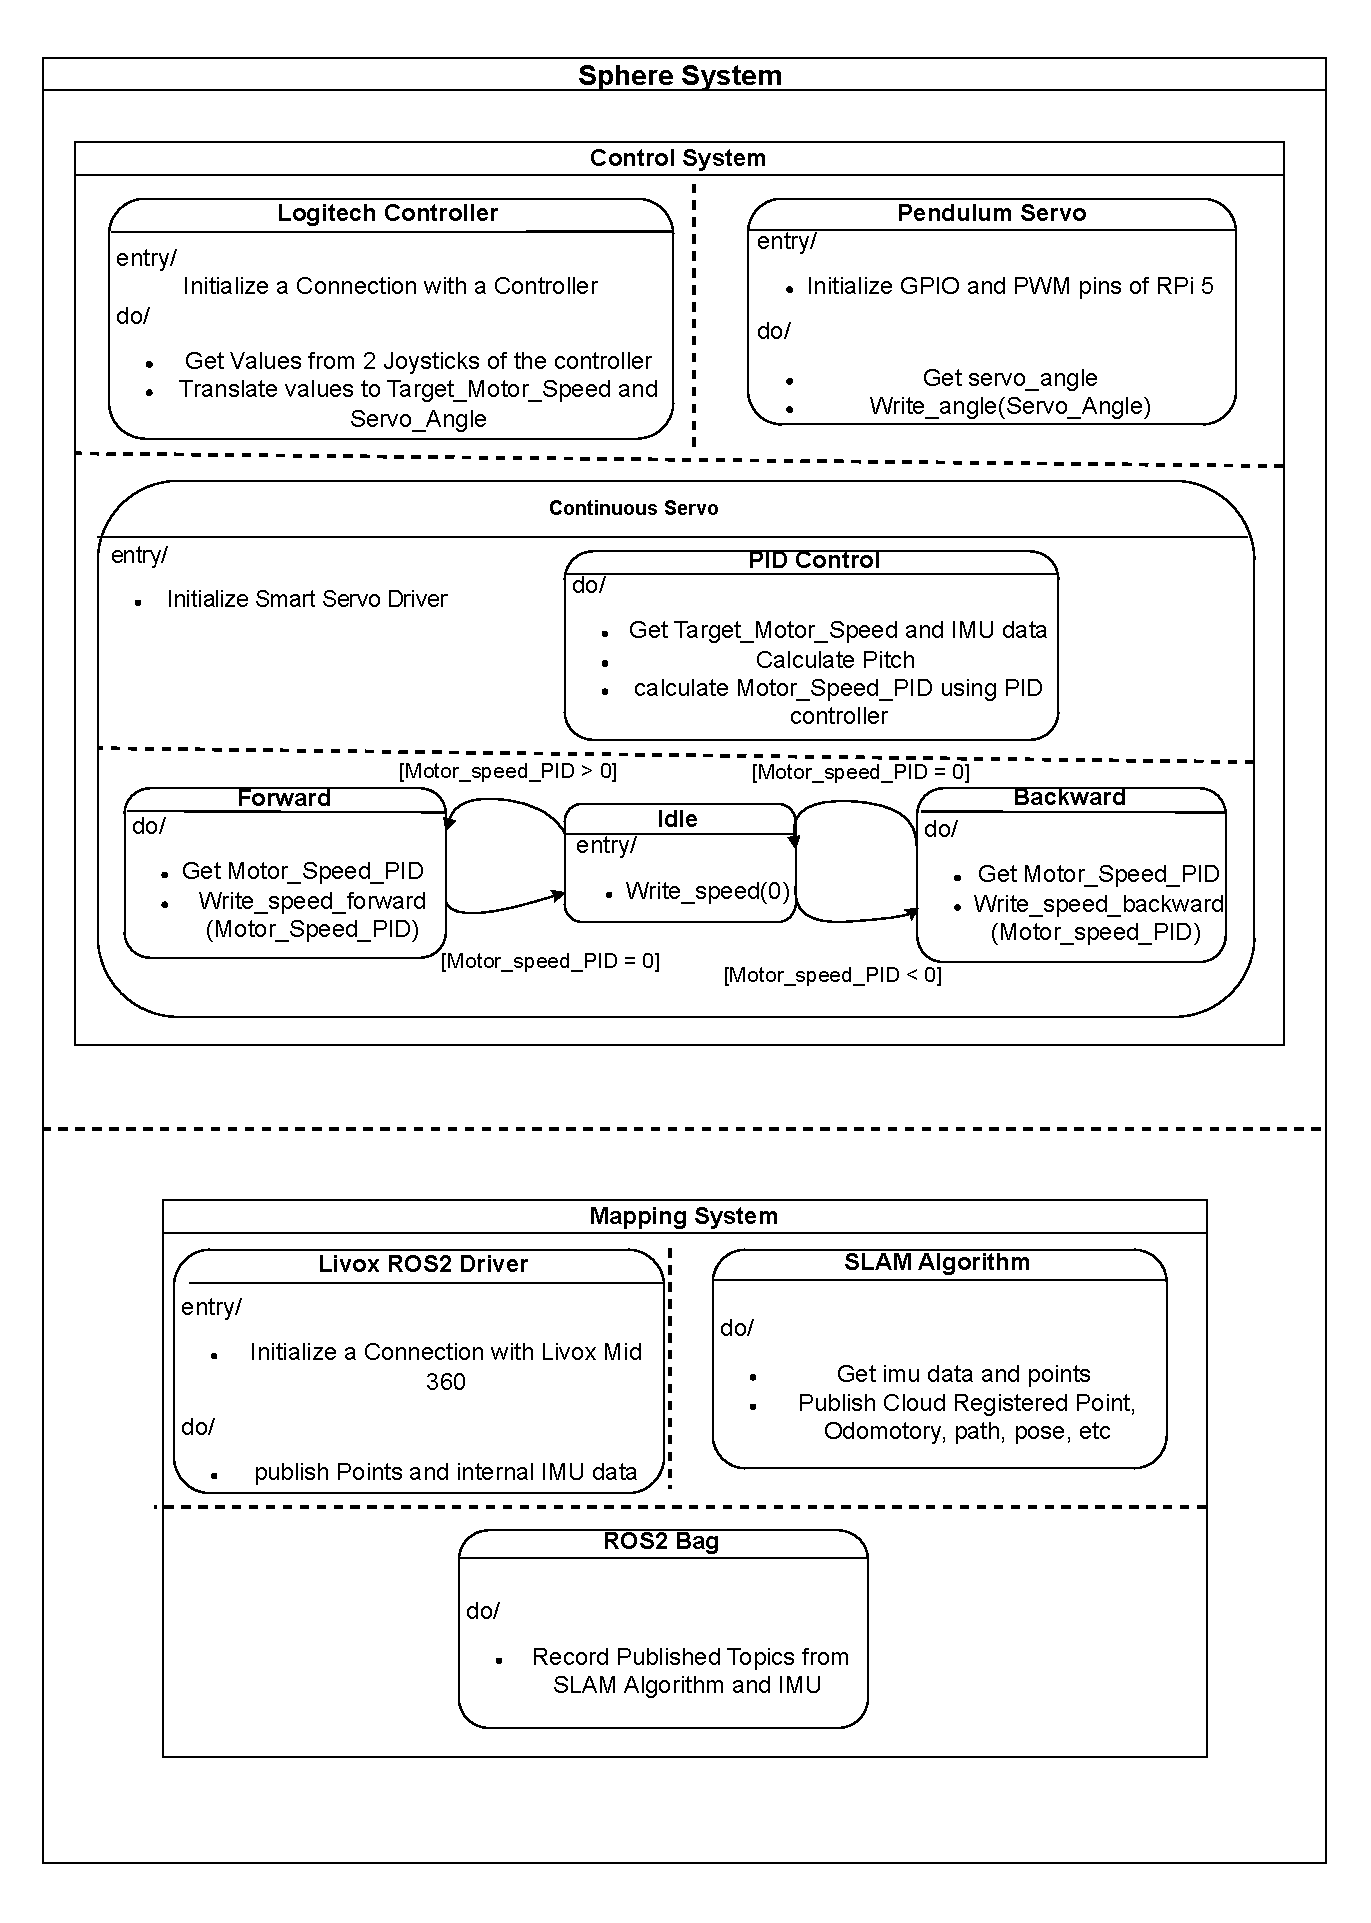
\includegraphics[width=0.95\linewidth]{pics/Khonsu_vertical.pdf} 
    \caption{State chart of the sphere system showing the control and mapping subsystems.}
    \label{fig:sphere_system}
\end{figure*}

As shown in the system state diagram in Fig.~\ref{fig:sphere_system}, both the actuated and non-actuated spheres follow the same state transitions, with the exception of the control subsystem, which is unique to the actuated variant. 
All software components are deployed on Ubuntu 24.04.2 LTS ARM and ROS2 Jazzy.

\section{Real-time Performance Optimization}
% Raspberry Pi 5 performance tuning
To ensure getting the most out of the Raspberry Pi 5, we applied several performance optimizations by using cooling fans on the Raspberry Pi and taking advantage of the PCIe bus to connect an NVMe HAT for improved data throughput.

One of the difficulties we faced was the limiting CPU performance of the Raspberry Pi 5 when not using the official 5V 5A power supply, as no official portable version exists. 
The official power supply is required to run the Raspberry Pi 5 at full performance~\cite{raspberrypi_psu}.
The Raspberry Pi 5 requires a minimum of 5V at 5A to operate at maximum CPU frequency and avoid performance throttling.

To address this, we used a 5V 5A voltage regulator to power the Raspberry Pi 5, and disabled the power delivery (PD) protocol to allow for higher power draw.
This modification enabled the system to maintain peak performance during intensive SLAM computations while operating on battery power within the spherical platform.

% Memory management strategies
% Processing pipeline optimization

\section{Mapping System}
Both spheres incorporate a real-time mapping system. 
The following LiDAR-Inertial Odometry (LIO) frameworks were evaluated and integrated:
\begin{itemize}
    \item \textbf{FAST-LIO2}
    \item \textbf{DLIO}
    \item \textbf{FAST-LIVO2} (LIO-only mode for real-time mapping)
\end{itemize}

Some packages such as \texttt{FAST-LIVO2} needed modification to meet the constraints and processing capabilities of the Raspberry Pi 5 and ROS2 Jazzy.
The mapping system is designed to operate in real-time, processing LiDAR scans and IMU data published from the Livox Mid-360 and BNO-085 sensors, respectively.
IMU data was collected from both the BNO-085 and Livox Mid-360, but only the Livox IMU data was used for mapping, as it is more reliable, which will be discussed in Chapter~\ref{ch:evaluation}.
The mapping system is implemented with several bash scripts that orchestrate the mapping pipeline, which processes the data using the selected LIO framework and publishes the resulting map in ROS bag format for later evaluation and comparison against ground truth data.
The source code, configuration files, and instructions for building the software are available in our GitHub repository~\cite{githubsphere}.
All mapping computations are performed onboard in real-time.

Figures~\ref{fig:ros_fast_lio}, \ref{fig:ros_fast_livo}, and \ref{fig:ros_dlio} show the Rqt graphs of the mapping system for each LIO framework, respectively.
Tables~\ref{tab:Livox_topics}, \ref{tab:fast_lio_topics}, \ref{tab:fast_livo_topics}, and \ref{tab:dlio_topics} summarize the key ROS2 topics used in the mapping system for each framework and Point-Cloud visualization.
\begin{figure}[H]
    \centering
    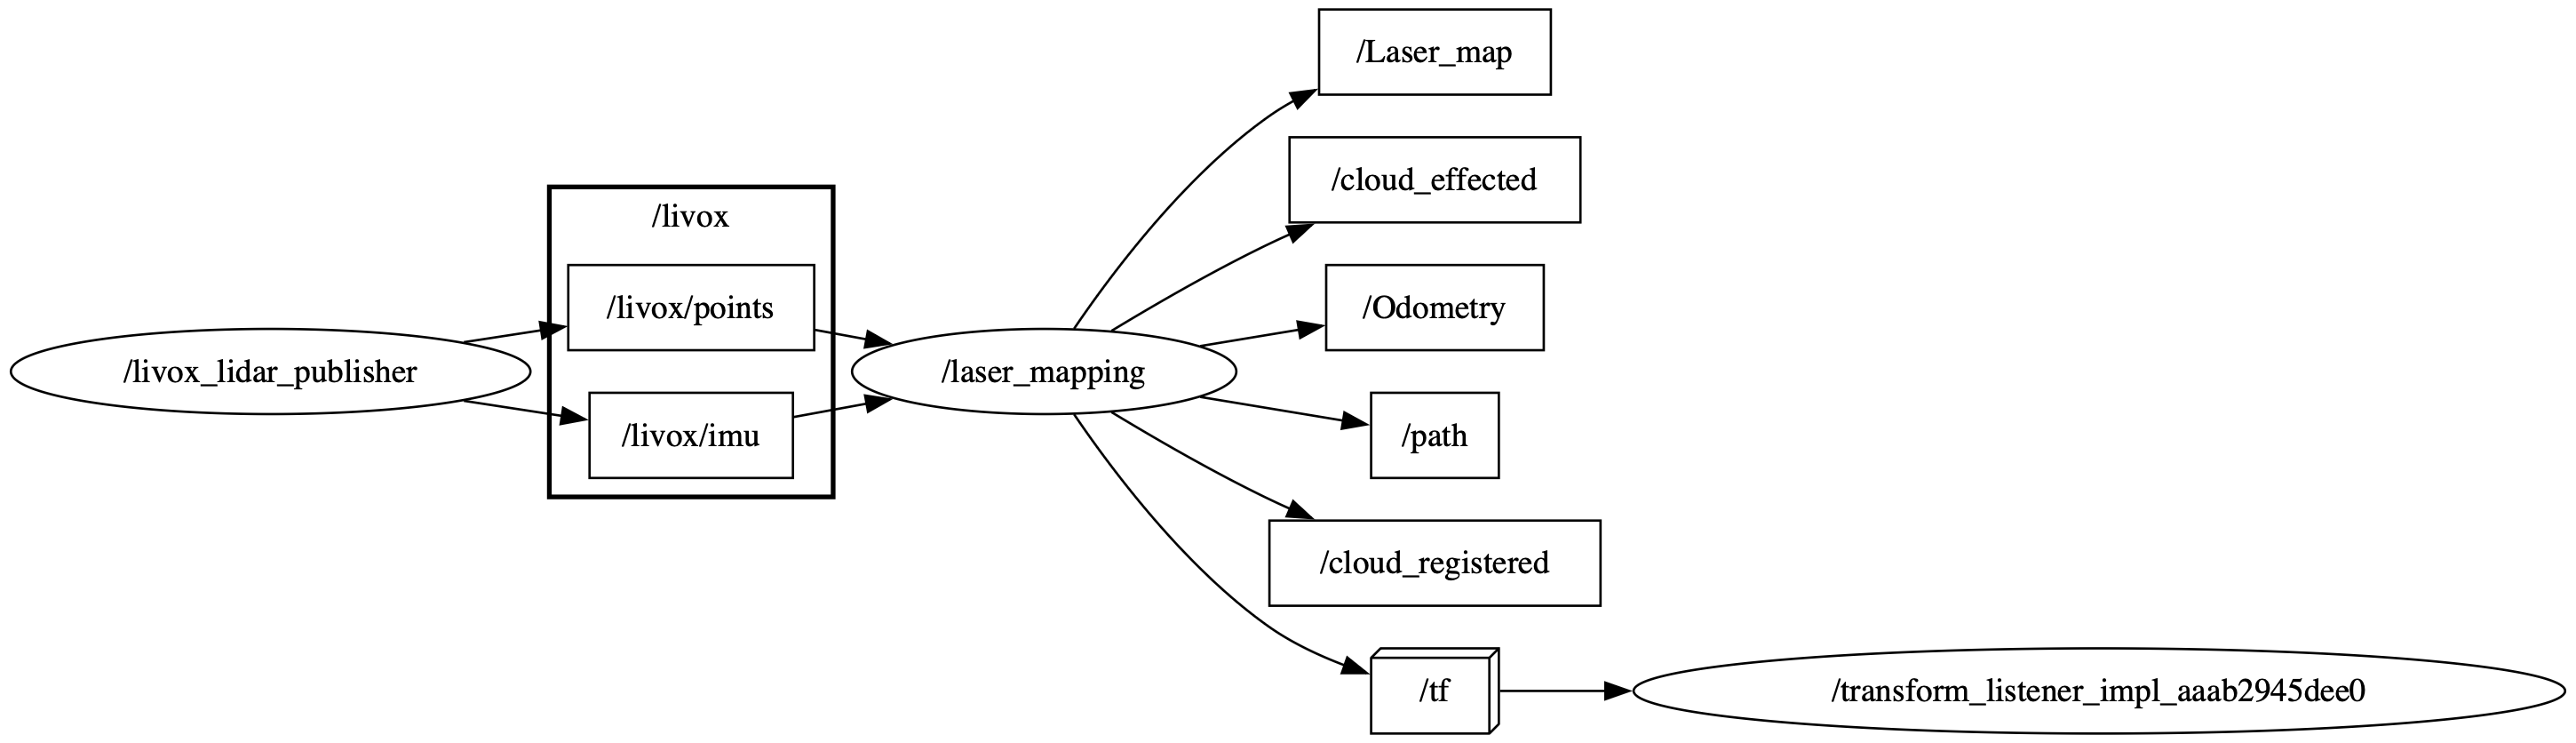
\includegraphics[width=\textwidth]{pics/rqt/ros_fast_lio.png}
    \caption{Mapping System Rqt Graph(FAST-LIO2)}
    \label{fig:ros_fast_lio}
\end{figure}




\begin{table}[ht]
\centering
\caption{Livox ROS2 Topics}
\label{tab:Livox_topics}
\scriptsize  % Even smaller than footnotesize
\begin{tabularx}{\textwidth}{@{}llXlX@{}}
\toprule
\textbf{Topic} & \textbf{Publisher} & \textbf{Subscribers} & \textbf{Type} & \textbf{Description} \\
\midrule
\texttt{/livox/imu} & \texttt{livox\_lidar\_publisher} & \texttt{waveshare\_servo\_node}, \texttt{laser\_mapping}, \texttt{dlio\_odom\_node} & \texttt{sensor\_msgs/Imu} & IMU data from internal IMU of Livox Mid-360 \\[0.3em]
\texttt{/livox/points} & \texttt{livox\_lidar\_publisher} & \texttt{laser\_mapping}, \texttt{dlio\_odom\_node} & \begin{tabular}{@{}l@{}}\texttt{sensor\_msgs/PointCloud2} \\ \texttt{livox\_ros\_driver2/CustomMsg}\end{tabular} & Point cloud data from Livox Mid-360 LiDAR \\
\bottomrule
\end{tabularx}
\end{table}

\begin{table}[H]
\centering
\caption{FAST-LIO2 ROS2 Topics}
\label{tab:fast_lio_topics}
\scriptsize  % Even smaller than footnotesize
\begin{tabularx}{\textwidth}{@{}llXlX@{}}
\toprule
\textbf{Topic} & \textbf{Publisher} & \textbf{Subscribers} & \textbf{Type} & \textbf{Description} \\
\midrule
\texttt{/Odometry} & \texttt{laser\_mapping} & rviz or rosbag & \texttt{nav\_msgs/Odometry} & publishes pose (position + orientation) and velocity of the robot \\[0.3em]
\texttt{/cloud\_registered} & \texttt{laser\_mapping} & rviz or rosbag & \texttt{sensor\_msgs/PointCloud2} & PointCloud data output from FAST-LIO2 \\
\texttt{/path} & \texttt{laser\_mapping} & rviz or rosbag & \texttt{nav\_msgs/Path} & Visualizes the full trajectory of the robot \\
\texttt{/tf} & \texttt{laser\_mapping} & rviz or rosbag & \texttt{tf2\_msgs/TFMessage} & Publishes the robot’s pose as a transform between frames (body -\textgreater~ camera\_init) \\

\bottomrule
\end{tabularx}
\end{table}
\begin{figure}[H]
    \centering
    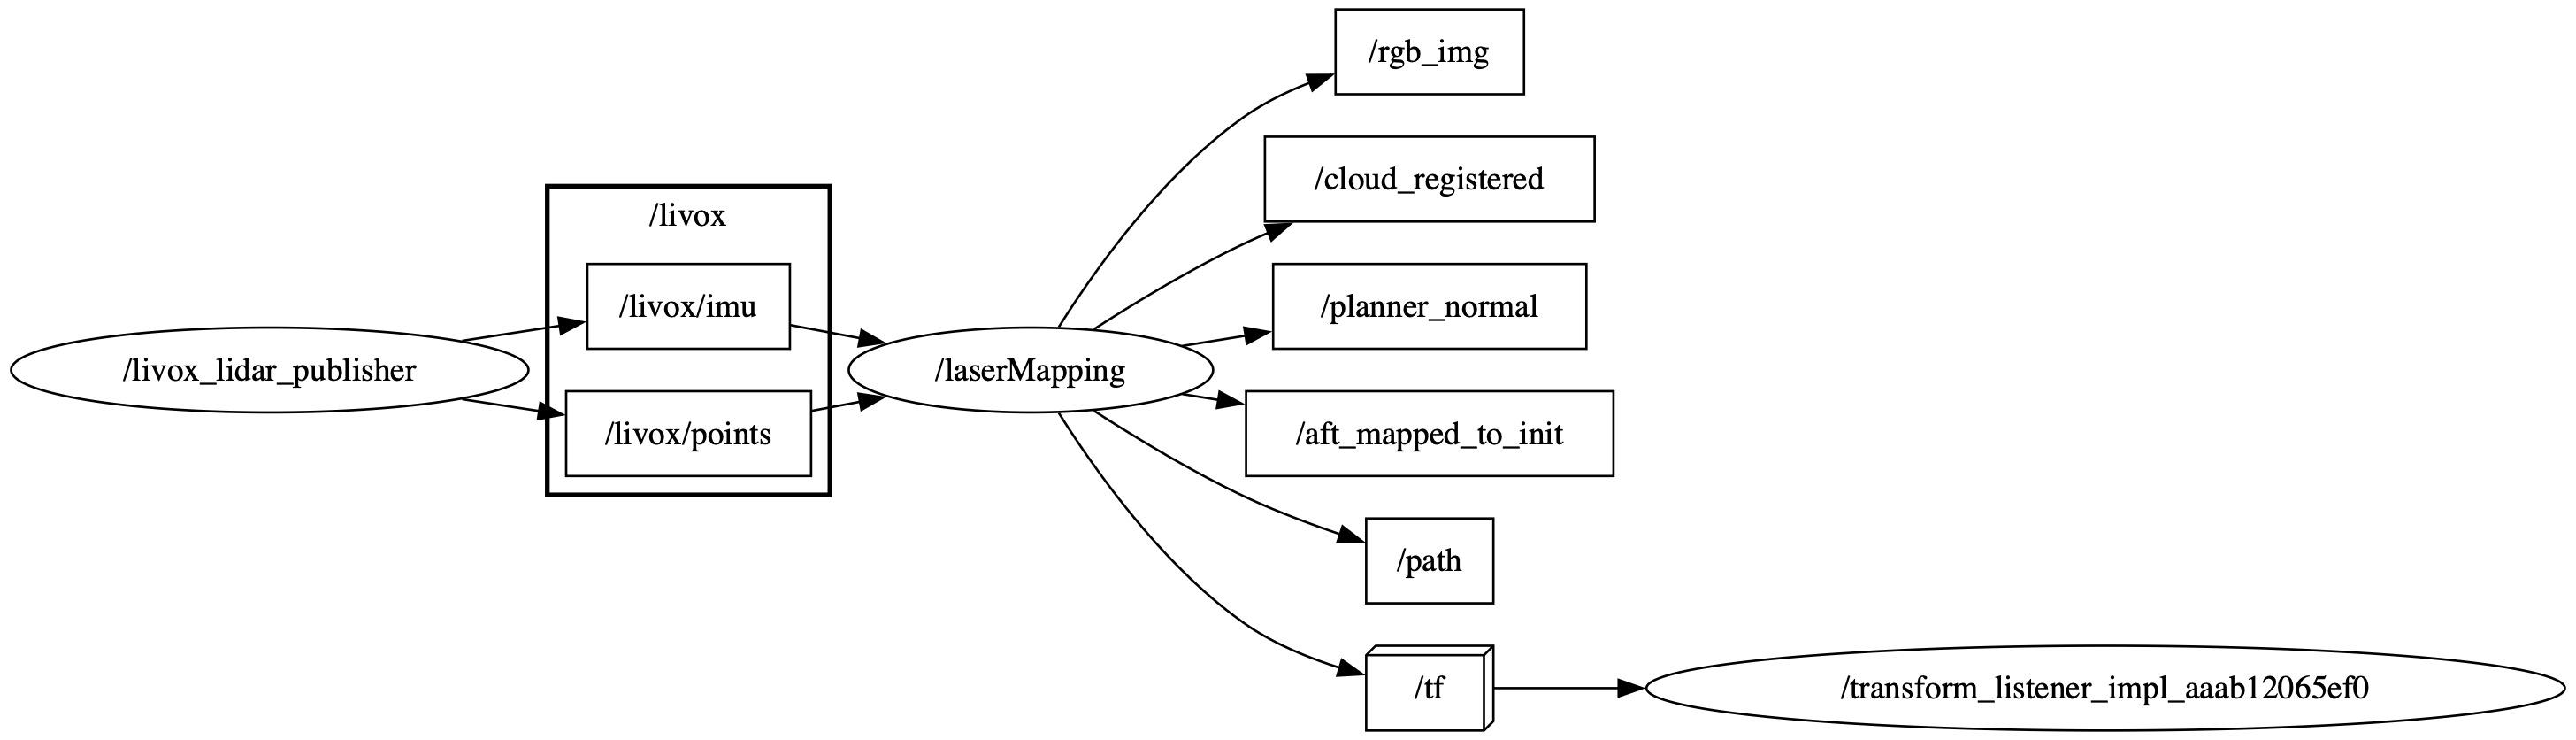
\includegraphics[width=\textwidth]{pics/rqt/ros_fast_livo.png}
    \caption{Mapping System Rqt Graph(FAST-LIVO2)}
    \label{fig:ros_fast_livo}
\end{figure}

\begin{table}[H]
\centering
\caption{FAST-LIVO2 ROS2 Topics}
\label{tab:fast_livo_topics}
\scriptsize  % Even smaller than footnotesize
\begin{tabularx}{\textwidth}{@{}llXlX@{}}
\toprule
\textbf{Topic} & \textbf{Publisher} & \textbf{Subscribers} & \textbf{Type} & \textbf{Description} \\
\midrule
\texttt{/cloud\_registered} & \texttt{laserMapping} & rviz or rosbag & \begin{tabular}{@{}l@{}}\texttt{sensor\_msgs/PointCloud2}\end{tabular}  & PointCloud data output from FAST-LIVO2 \\[0.3em]
\texttt{/path} & \texttt{laserMapping} & rviz or rosbag & \texttt{nav\_msgs/Path} & Visualizes the full trajectory of the robot \\
\texttt{/tf} & \texttt{laserMapping} & rviz or rosbag & \texttt{tf2\_msgs/TFMessage} & Publishes the robot’s pose as a transform between frames (aft\_mapped -\textgreater~ camera\_init) \\

\bottomrule
\end{tabularx}
\end{table}



\clearpage

\begin{figure}[H]
    \centering
    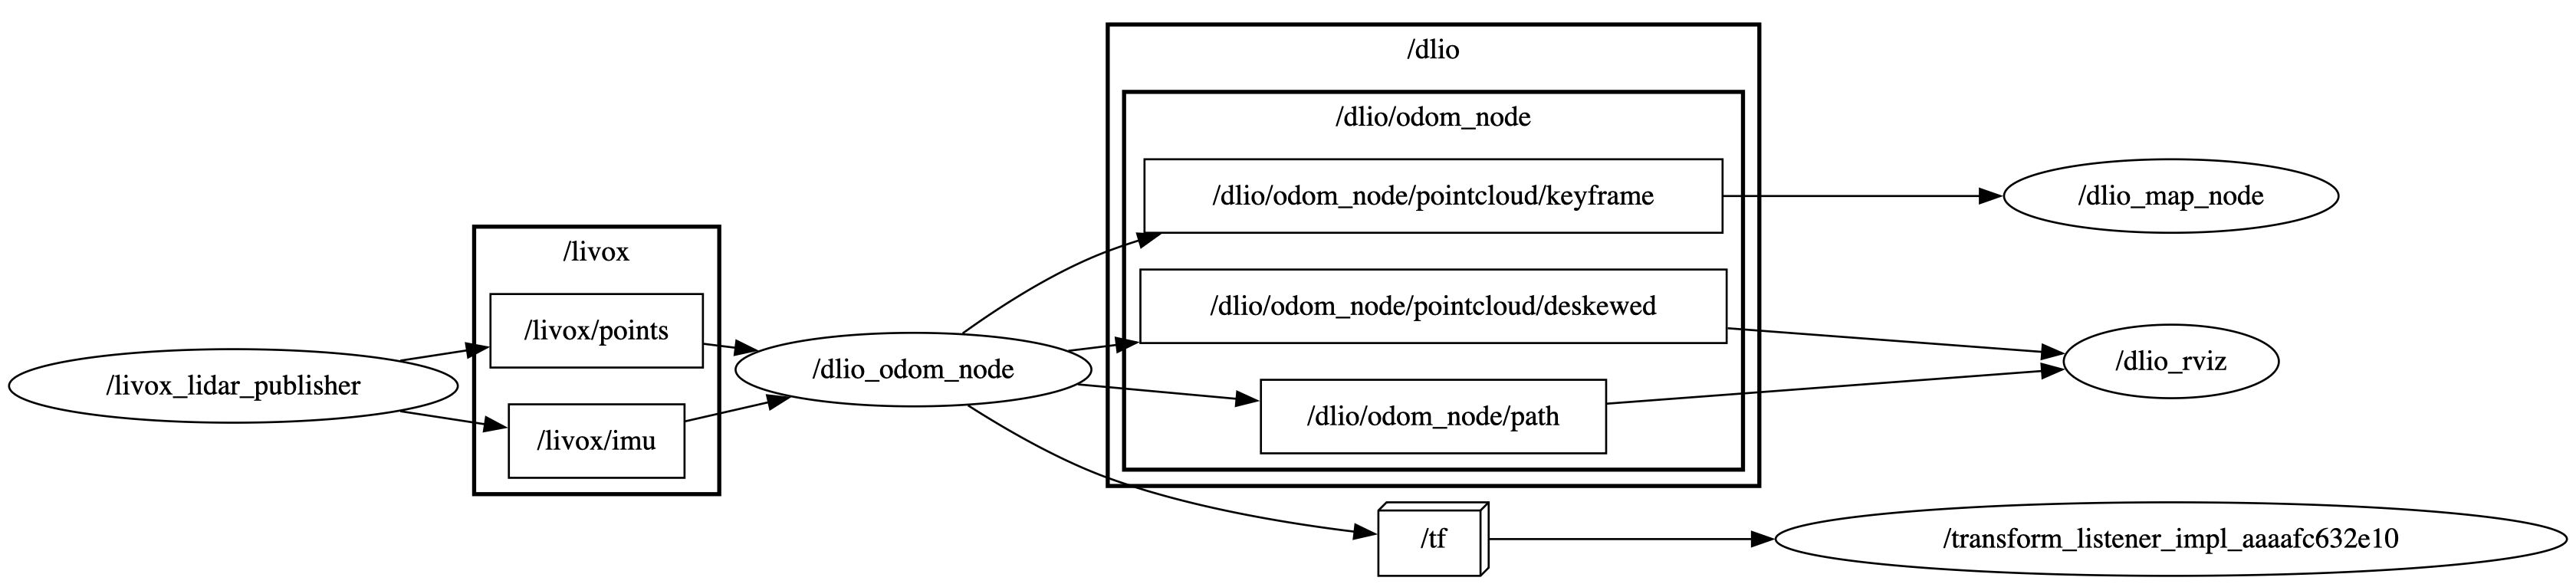
\includegraphics[width=\textwidth]{pics/rqt/ros_dlio.png}
    \caption{Mapping System Rqt Graph(DLIO)}
    \label{fig:ros_dlio}
\end{figure}

\begin{table}[H]
\centering
\caption{DLIO ROS2 Topics}
\label{tab:dlio_topics}
\scriptsize  % Even smaller than footnotesize
\begin{tabularx}{\textwidth}{@{}llXlX@{}}
\toprule
\textbf{Topic} & \textbf{Publisher} & \textbf{Subscribers} & \textbf{Type} & \textbf{Description} \\
\midrule
\texttt{/dlio/odom\_node/pointcloud/deskewed} & \texttt{dlio\_odom\_node} & rviz or rosbag & \texttt{sensor\_msgs/PointCloud2} & PointCloud data output from DLIO \\[0.3em]
\texttt{/dlio/odom\_node/path} & \texttt{dlio\_odom\_node} & rviz or rosbag & \texttt{nav\_msgs/Path} & Visualizes the full trajectory of the robot \\
\texttt{/tf} & \texttt{dlio\_odom\_node} & rviz or rosbag & \texttt{tf2\_msgs/TFMessage} & Publishes the robot’s pose as a transform between frames (odom -\textgreater~base\_link ) \\

\bottomrule
\end{tabularx}
\end{table}



\section{Actuator System (Actuated Sphere Only)}
The actuated sphere features an internal movement control system, operated using a Logitech F710 controller. 
The controller's two joysticks are mapped to distinct control tasks:
\begin{itemize}
    \item \textbf{Servo control:} One joystick provides input to the continuous rotation servo. 
    These inputs are scaled and passed through a discrete Proportional-Integral-Derivative (PID) controller to regulate pitch by minimizing the error between the desired target angle and the current angle measured by the IMU.
    \item \textbf{Mass shifting:} The second joystick adjusts the angle of an internal weight to shift the center of mass left or right, enabling directional control of the sphere's rolling behavior.
\end{itemize}
This control strategy allows for fine-grained movement and stabilization, combining feedback-based servo control with physical mass displacement for maneuvering.
% \begin{equation}
% u[k] = K_p \cdot e[k] + K_i \cdot \sum_{i=0}^{k} e[i] \cdot \Delta t + K_d \cdot \frac{e[k] - e[k-1]}{\Delta t} \label{eq:pid_control}
% \end{equation}
% where \( u[k] \) is the servo motor command at time step \( k \), \( e[k] \) is the pitch error defined as the difference between the target angle \( \theta_{\text{target}} \) and the current angle \( \theta_{\text{current}} \), and \( K_p \), \( K_i \), \( K_d \) are the proportional, integral, and derivative gains, respectively. The controller runs at a fixed sampling interval \( \Delta t \) and includes a small deadband around the setpoint to reduce oscillations. Within this deadband, the integral term is reset to prevent windup. Additionally, manual control inputs can be superimposed onto the PID output, enabling user intervention without disrupting balance. The resulting command is then limited to a predefined range before being sent to the servo motor, which also considers real-time motor speed and IMU feedback to maintain stable velocity and orientation.

The control system is implemented using three separate ROS2 packages but they are in same workspace, each responsible for a specific aspect of the control logic:
\begin{itemize}
    \item \texttt{waveshare\_servo}: Implements the PID control logic for the continuous servo motor and manages forward/backward movement.
    \item \texttt{logitech\_controller}: Handles joystick input from the Logitech F710 controller, translating joystick movements to control commands for pwm servo and waveshare servo operation and mass shifting.
    \item \texttt{servo\_pwm\_node}: Manages PWM signal generation for the servo motor using wiringPi with rapid GPIO access which is responsible for pendulum control and mass shifting.
\end{itemize} 
These packages are integrated to initialize using a single command from a master ROS package called \texttt{Khonsu}, which enables system activation with a single command.

Figures~\ref{fig:ros_actuator} shows the Rqt graph of the actuator system.
Table~\ref{tab:actuator_topics} summarizes the key ROS2 topics used in the actuator system.
\begin{figure}[H]
    \centering
    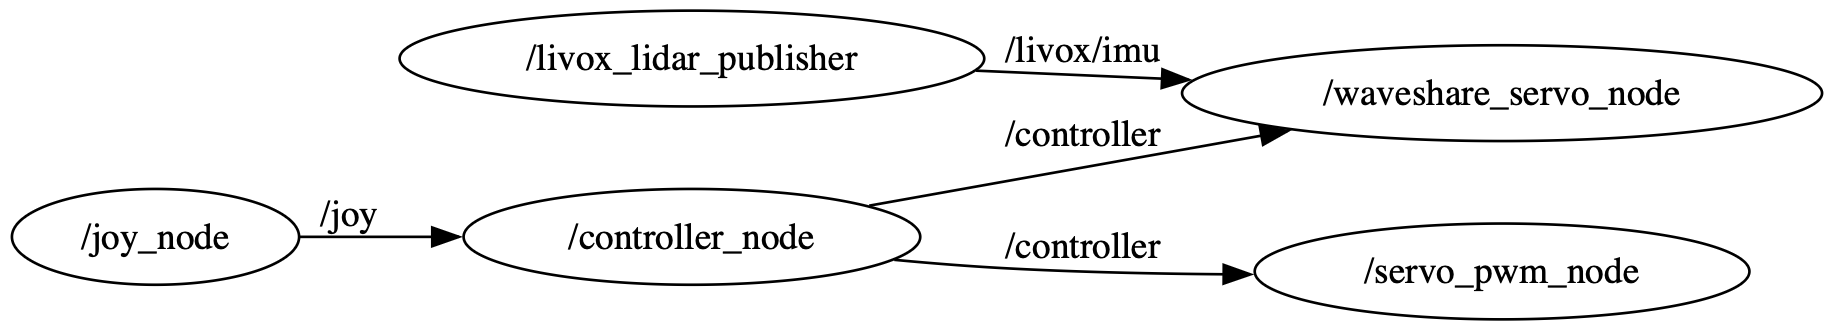
\includegraphics[width=\textwidth]{pics/rqt/ros_actuator.png}
    \caption{Actuator System Rqt Graph}
    \label{fig:ros_actuator}
\end{figure}

\begin{table}[H]
\centering
\caption{Actuator System ROS2 Topics}
\label{tab:actuator_topics}
\scriptsize
\begin{tabularx}{\textwidth}{@{}llXlX@{}}
\toprule
\textbf{Topic} & \textbf{Publisher} & \textbf{Subscribers} & \textbf{Type} & \textbf{Description} \\
\midrule
\texttt{/joy} & \texttt{joy\_node} & \texttt{controlled\_node} & \texttt{sensor\_msgs/Joy} & Joystick input data from Logitech F710 controller \\[0.3em]
\texttt{/controller} & \texttt{controller\_node} & \texttt{waveshare\_servo\_node}, \texttt{servo\_pwm\_node} & \texttt{logitech\_msgs/CustomMsg} & Control commands for servo motors and mass shifting \\
\bottomrule
\end{tabularx}
\end{table}


\chapter{Evaluation and Results}
\label{ch:evaluation}

In this Chapter, we present the evaluation and results of both spherical robots in terms of their mapping accuracy and stability.
All experiments were conducted in a controlled indoor environment within the Computer Science building at the University of Würzburg.

\section{Evaluation Setup}
The evaluation consisted of mapping selected indoor areas—specifically, a corridor, a hall, and the upper floor—using both the non-actuated and actuated spherical robots. 
For the non-actuated sphere, the robot was manually moved by hand and by foot. 
Each mapping run used one of three SLAM algorithms: FAST-LIO2, DLIO, and FAST-LIVO2 (LIO mode). 
The experiment was repeated three times—once for each algorithm—under the same environmental conditions. 
The same procedure was carried out with the actuated sphere, with the key difference being that it was moved using a controller rather than manually. 
Again, each of the three SLAM algorithms was executed along similar paths within the same locations. 
We used 3DTK~\cite{3dtk} to process the resulting point-clouds, which were evaluated by comparing them against ground truth data obtained using a Riegl VZ-400 terrestrial laser scanner (TLS) as shown in Fig.~\ref{fig:riegl}.
\begin{figure}[t]
\centering
\begin{subfigure}{0.495\columnwidth}
        \centering
        \includegraphics[width=\textwidth]{pics/riegl_lr.jpg}
        \caption{Riegl VZ-400}
        \label{fig:riegl}
\end{subfigure}
\hfill
\begin{subfigure}{0.49\columnwidth}
        \centering
        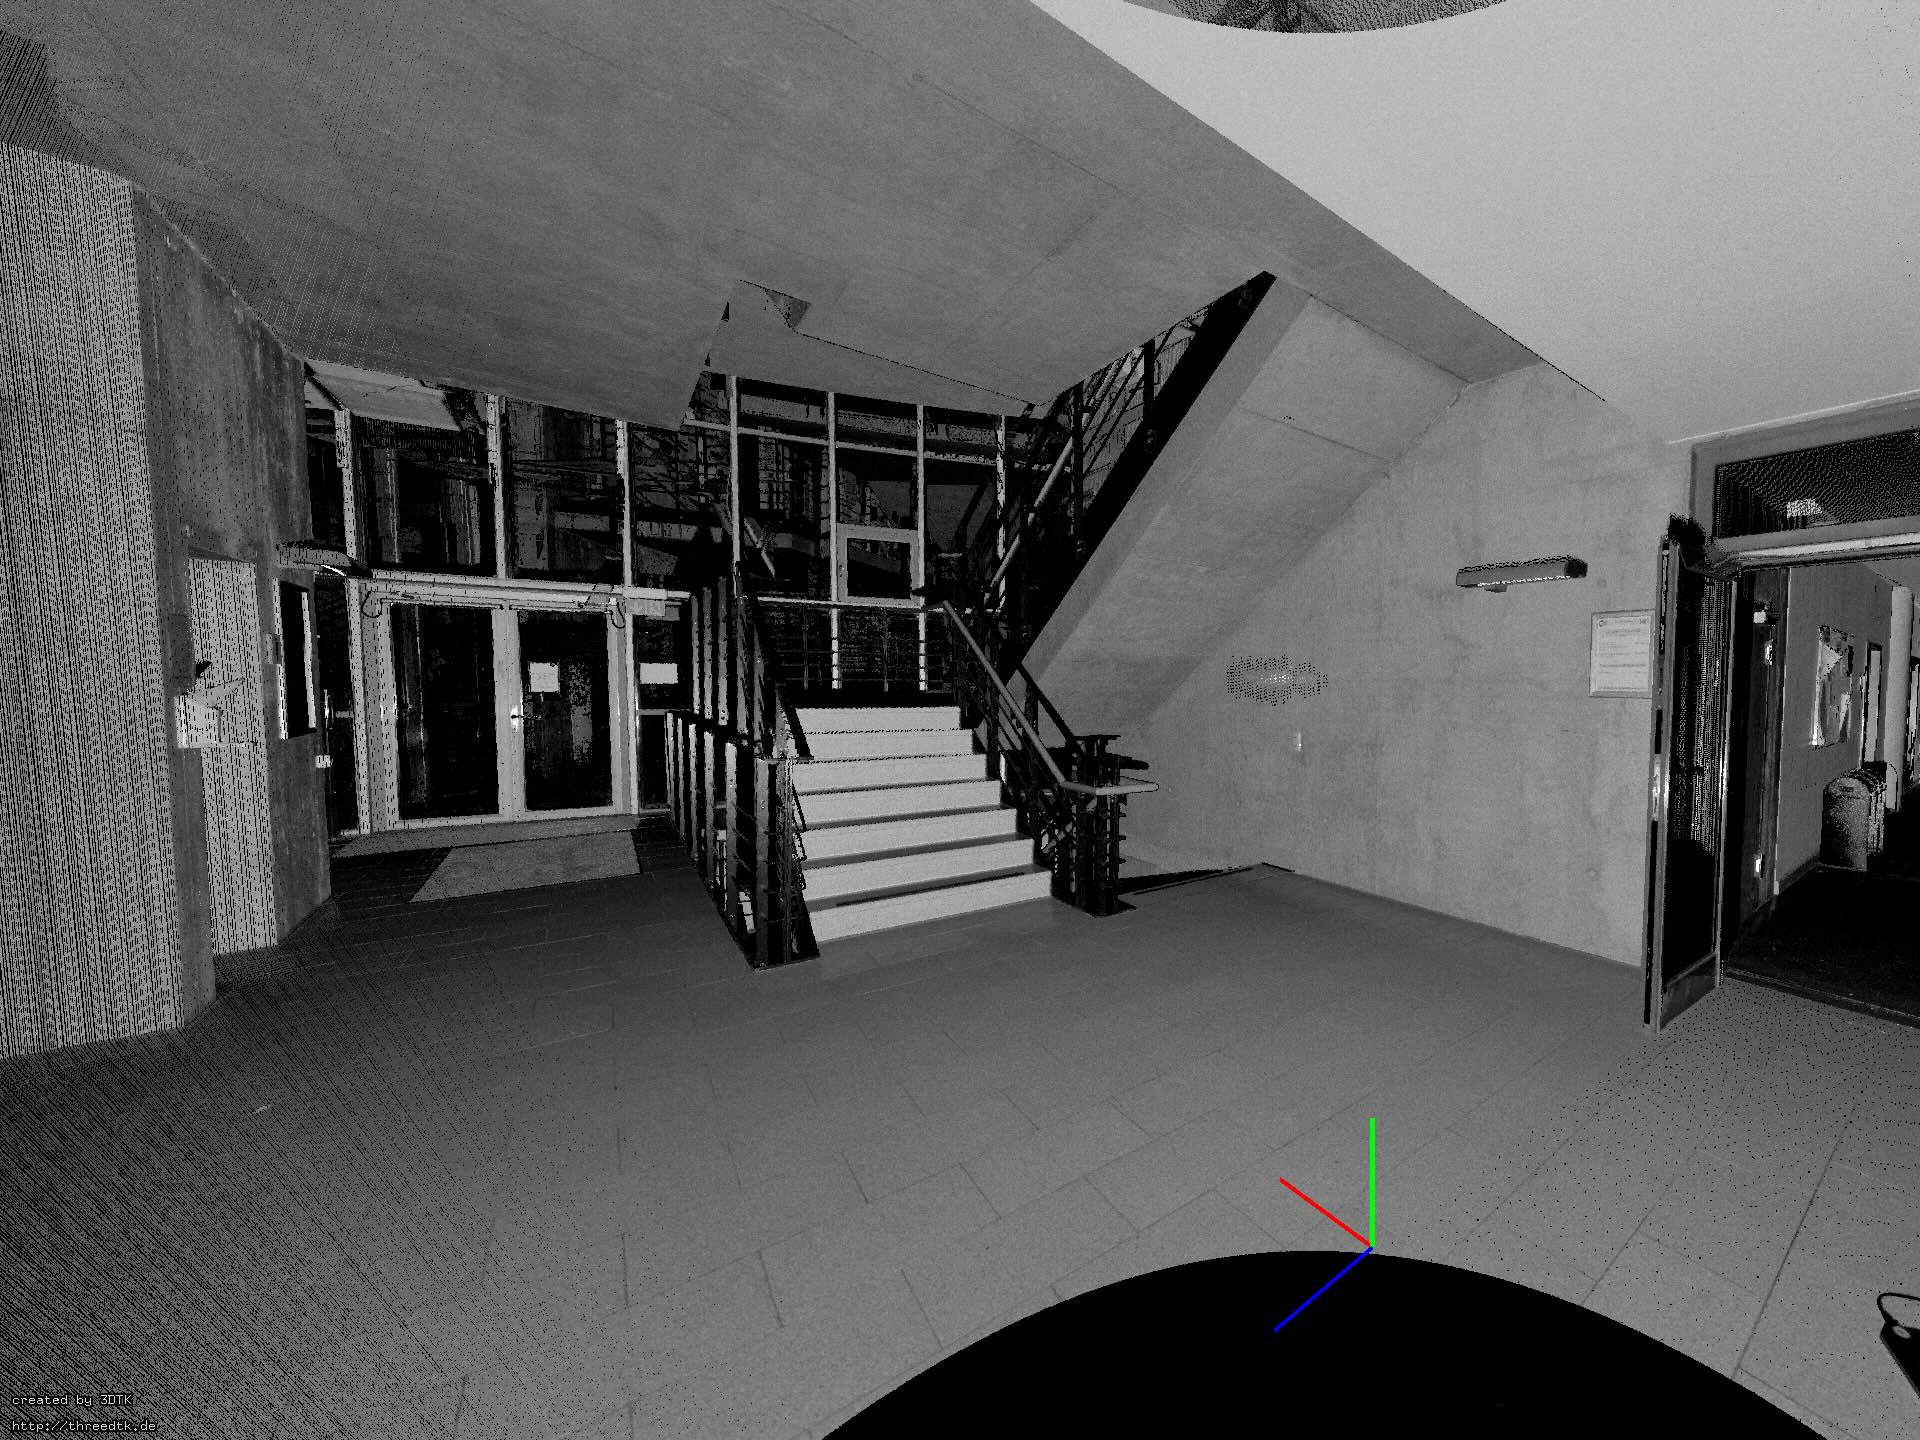
\includegraphics[width=\textwidth]{pics/groundtruth1.jpg}\vspace{.5mm}
        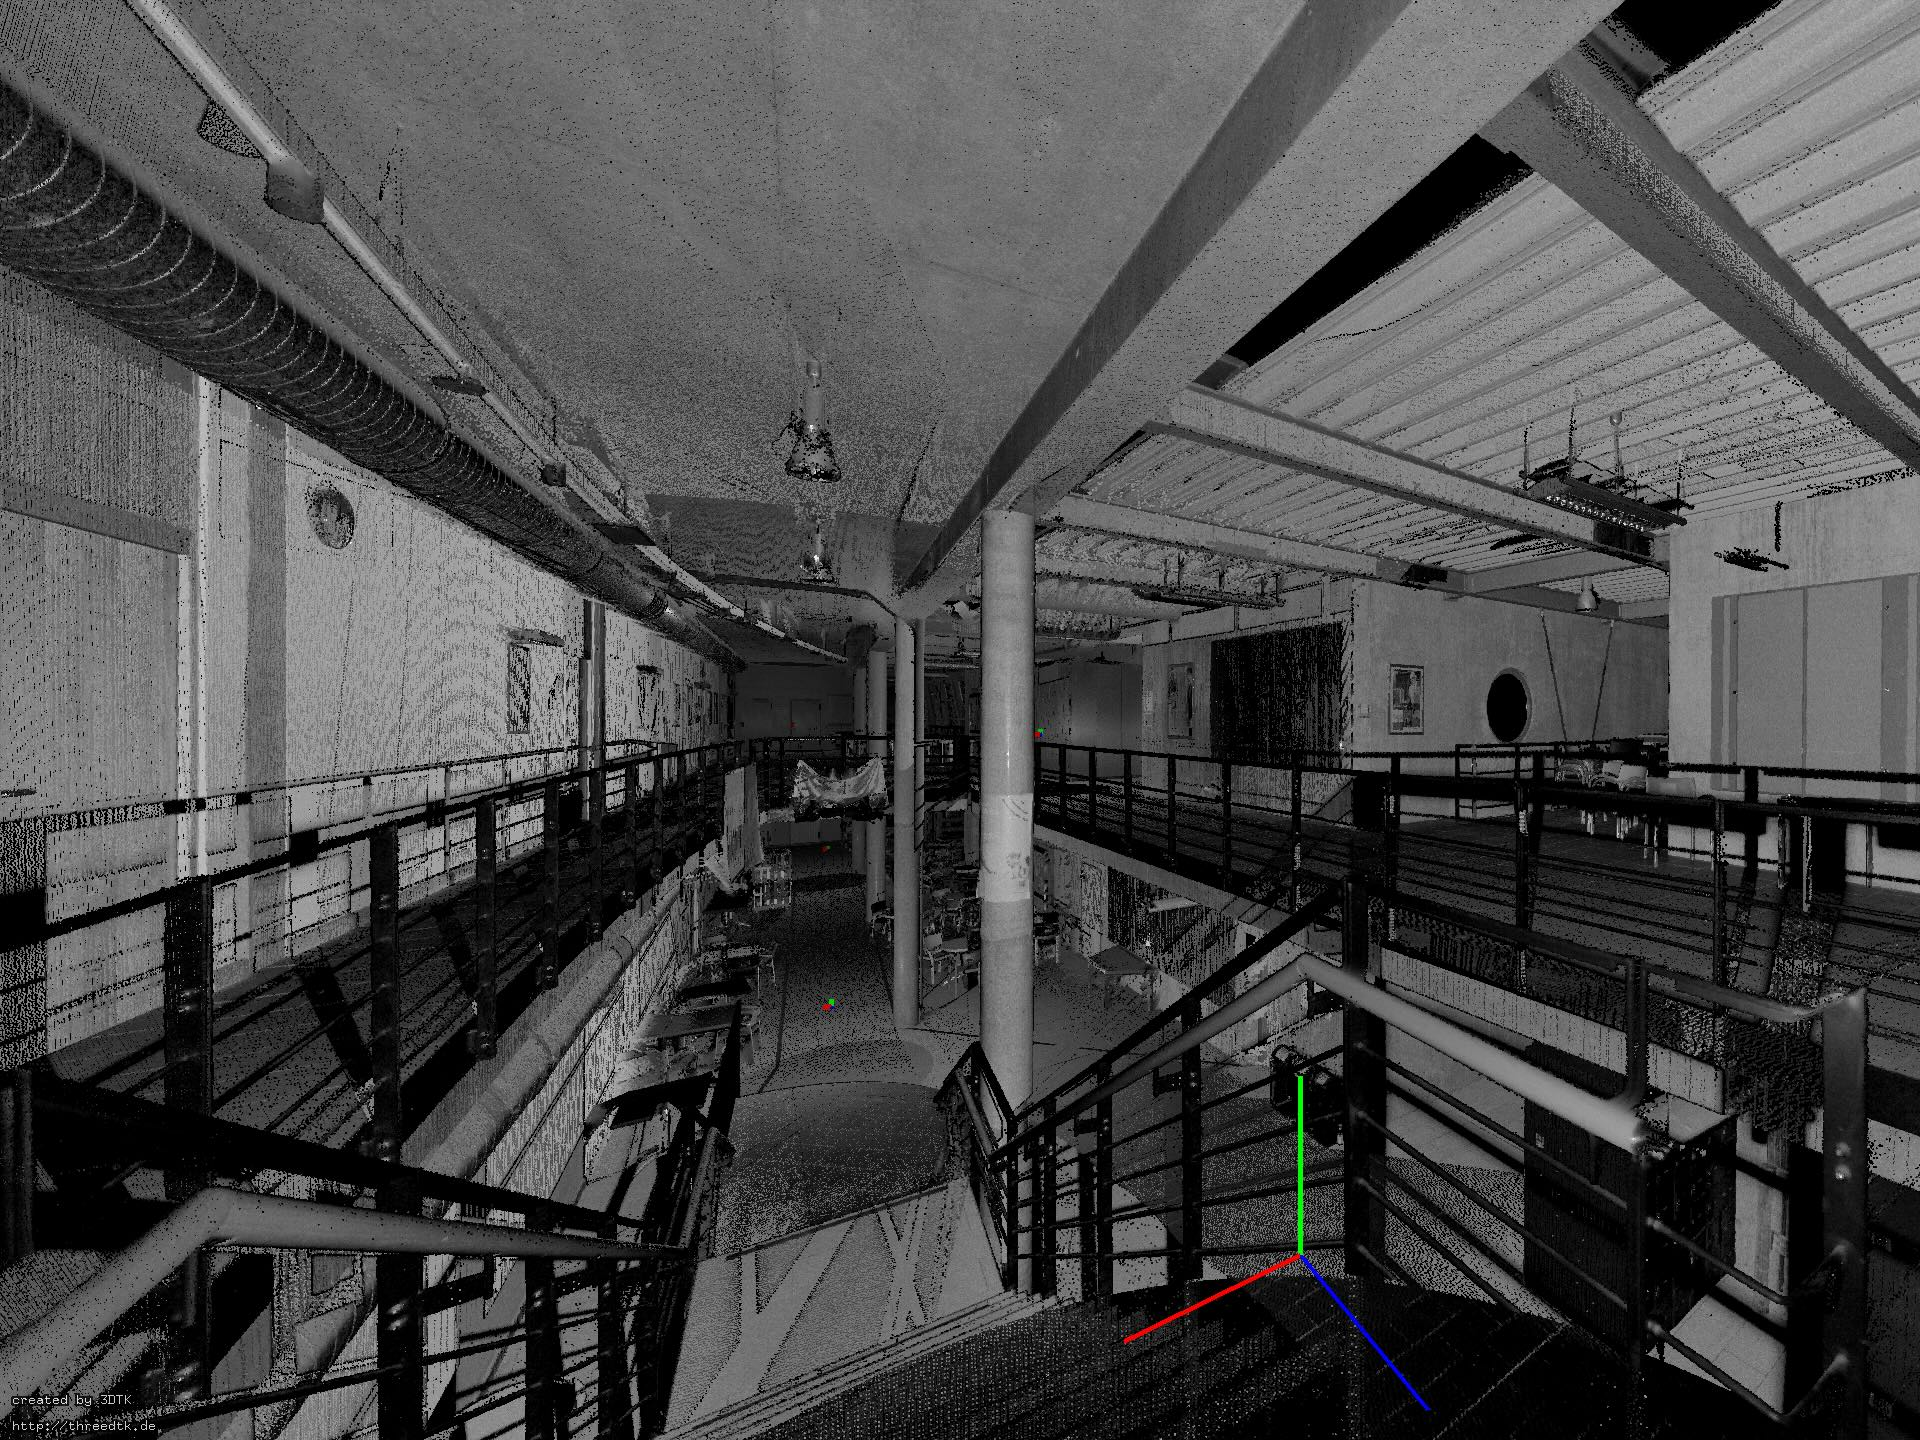
\includegraphics[width=\textwidth]{pics/groundtruth2.jpg}
        \caption{Ground truth point-clouds}
        \label{fig:sphere_on_the_move}
\end{subfigure}
\caption{Evaluation setup, showing the Riegl VZ-400 terrestrial laser scanner (TLS) and the resulting point-cloud used as ground truth in the evaluation.}\vspace{-3mm}
\end{figure}
\begin{figure}[t]
\centering
\begin{subfigure}{0.492\columnwidth}
        \centering
        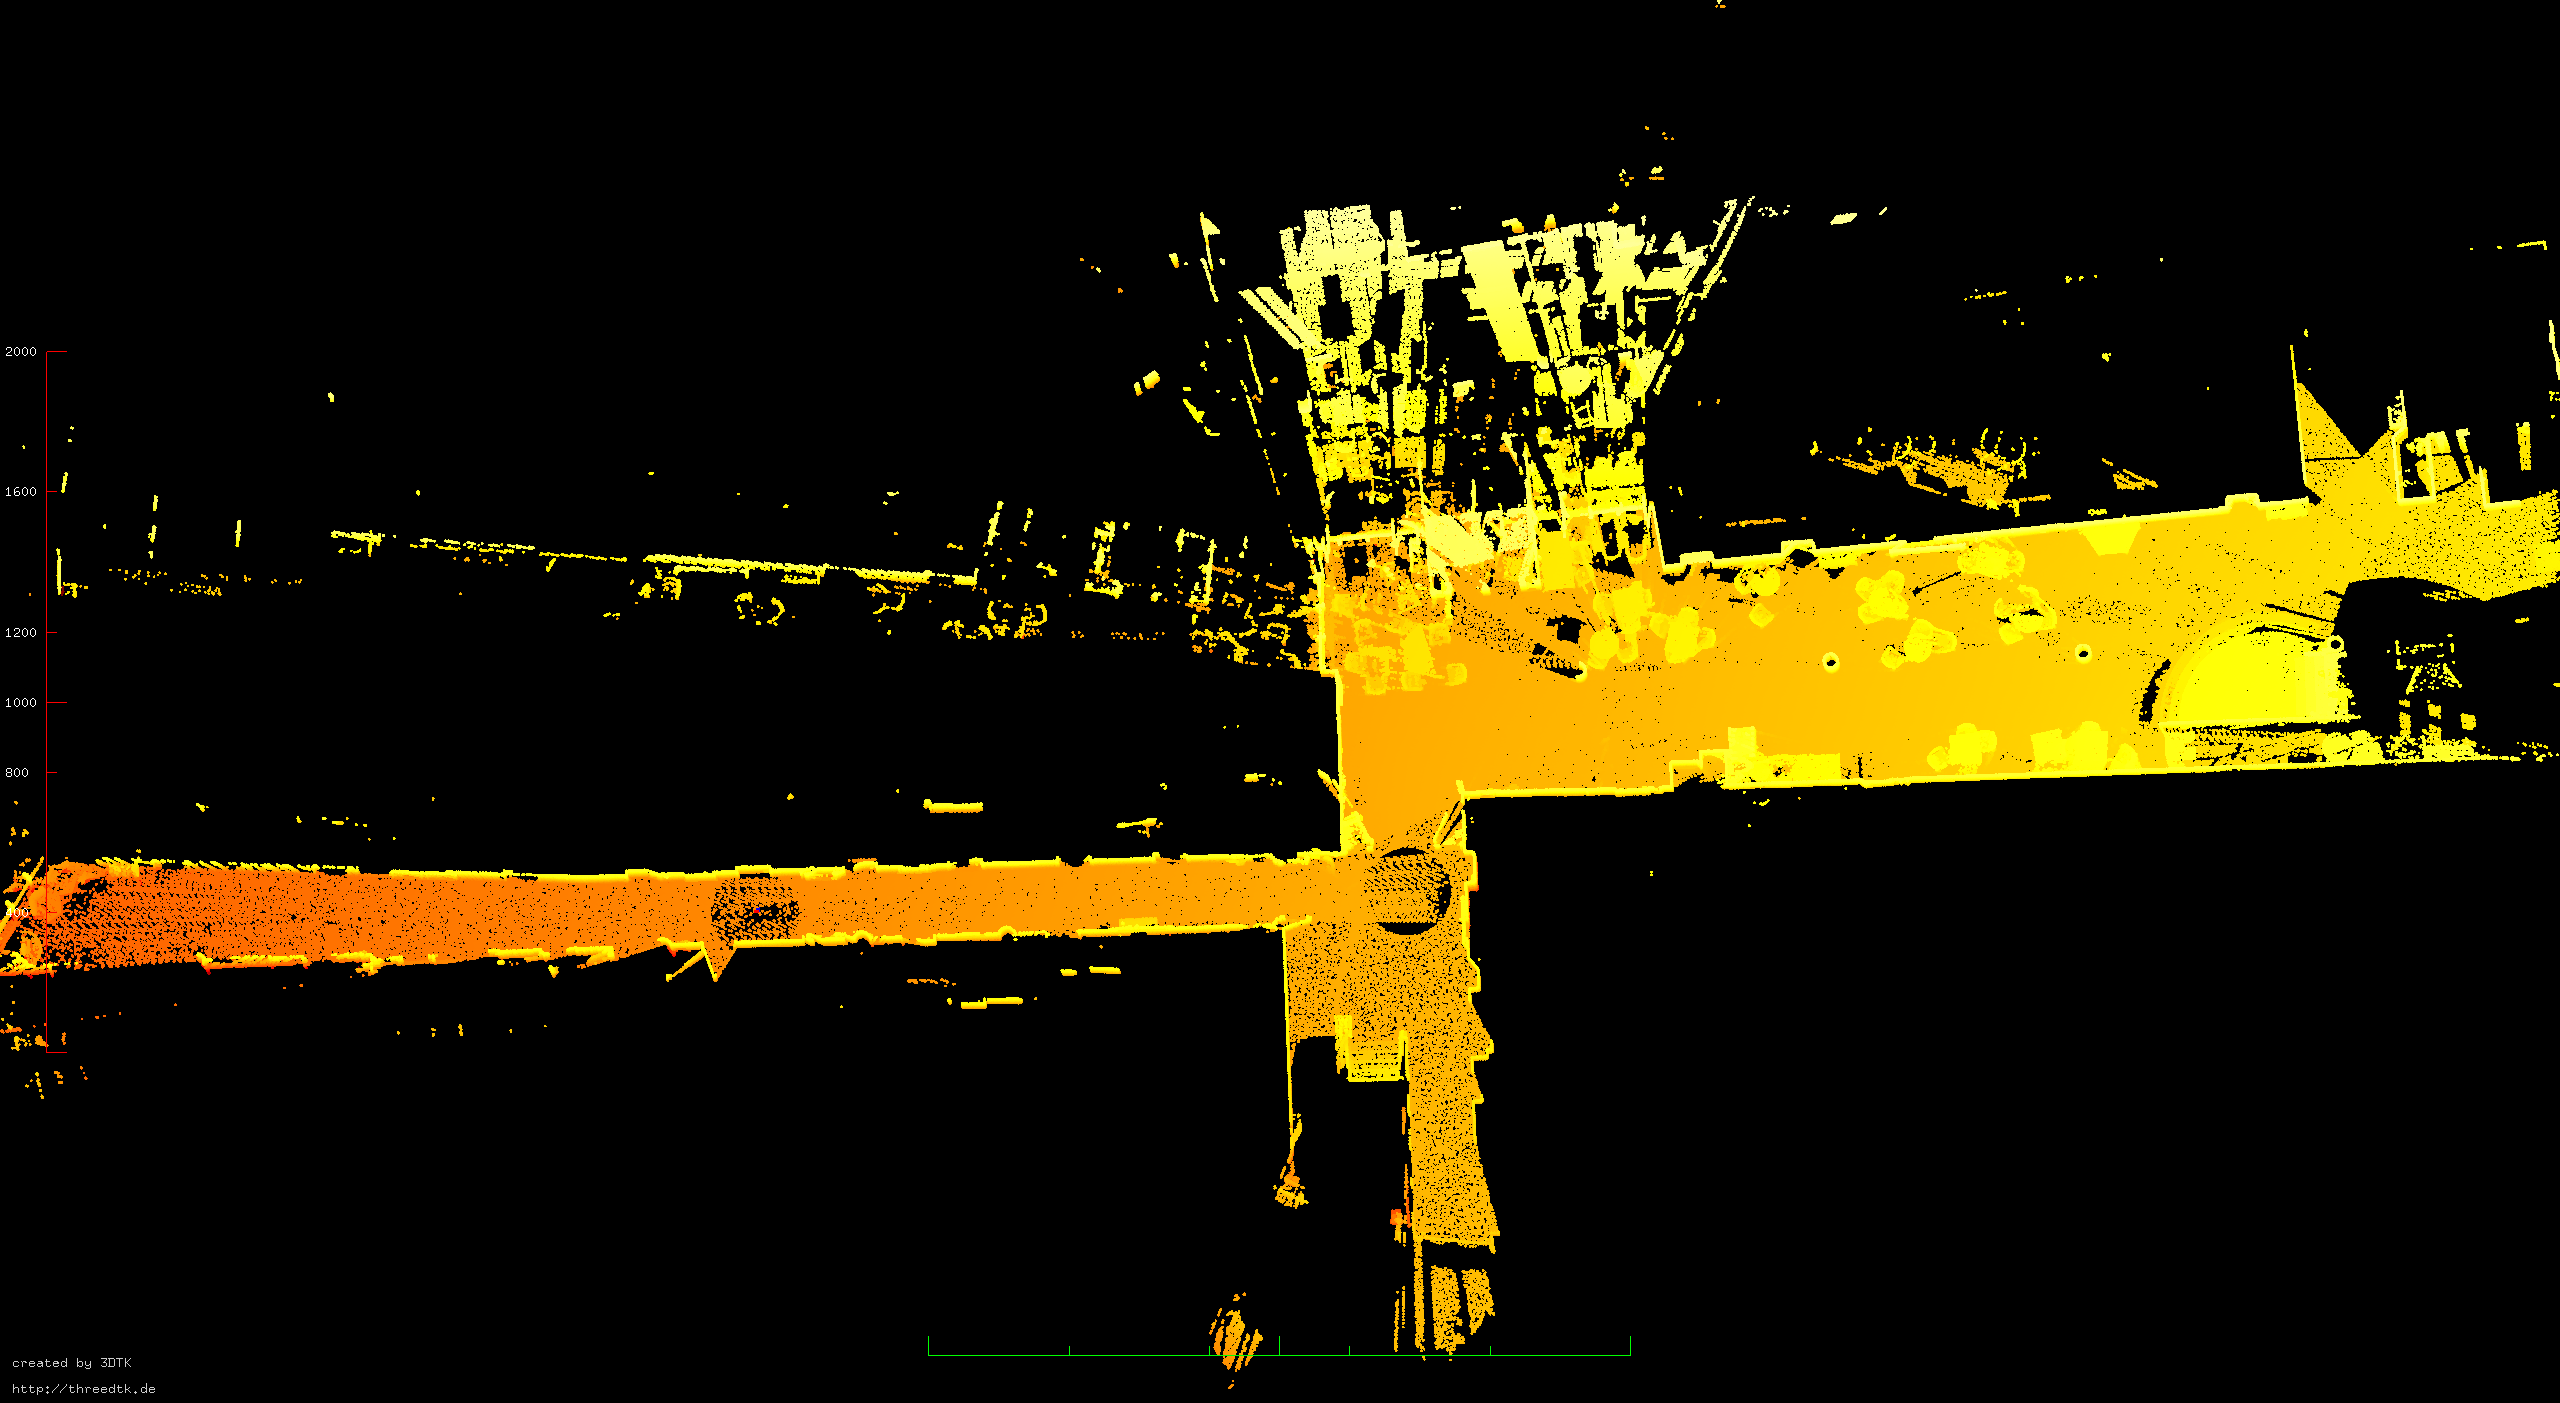
\includegraphics[width=\textwidth]{pics/eagle_view/riegl_top.png}
        \caption{Riegl Map Result}
        \label{fig:riegl_top}\end{subfigure}
\hfill
\begin{subfigure}{0.492\columnwidth}
        \centering
        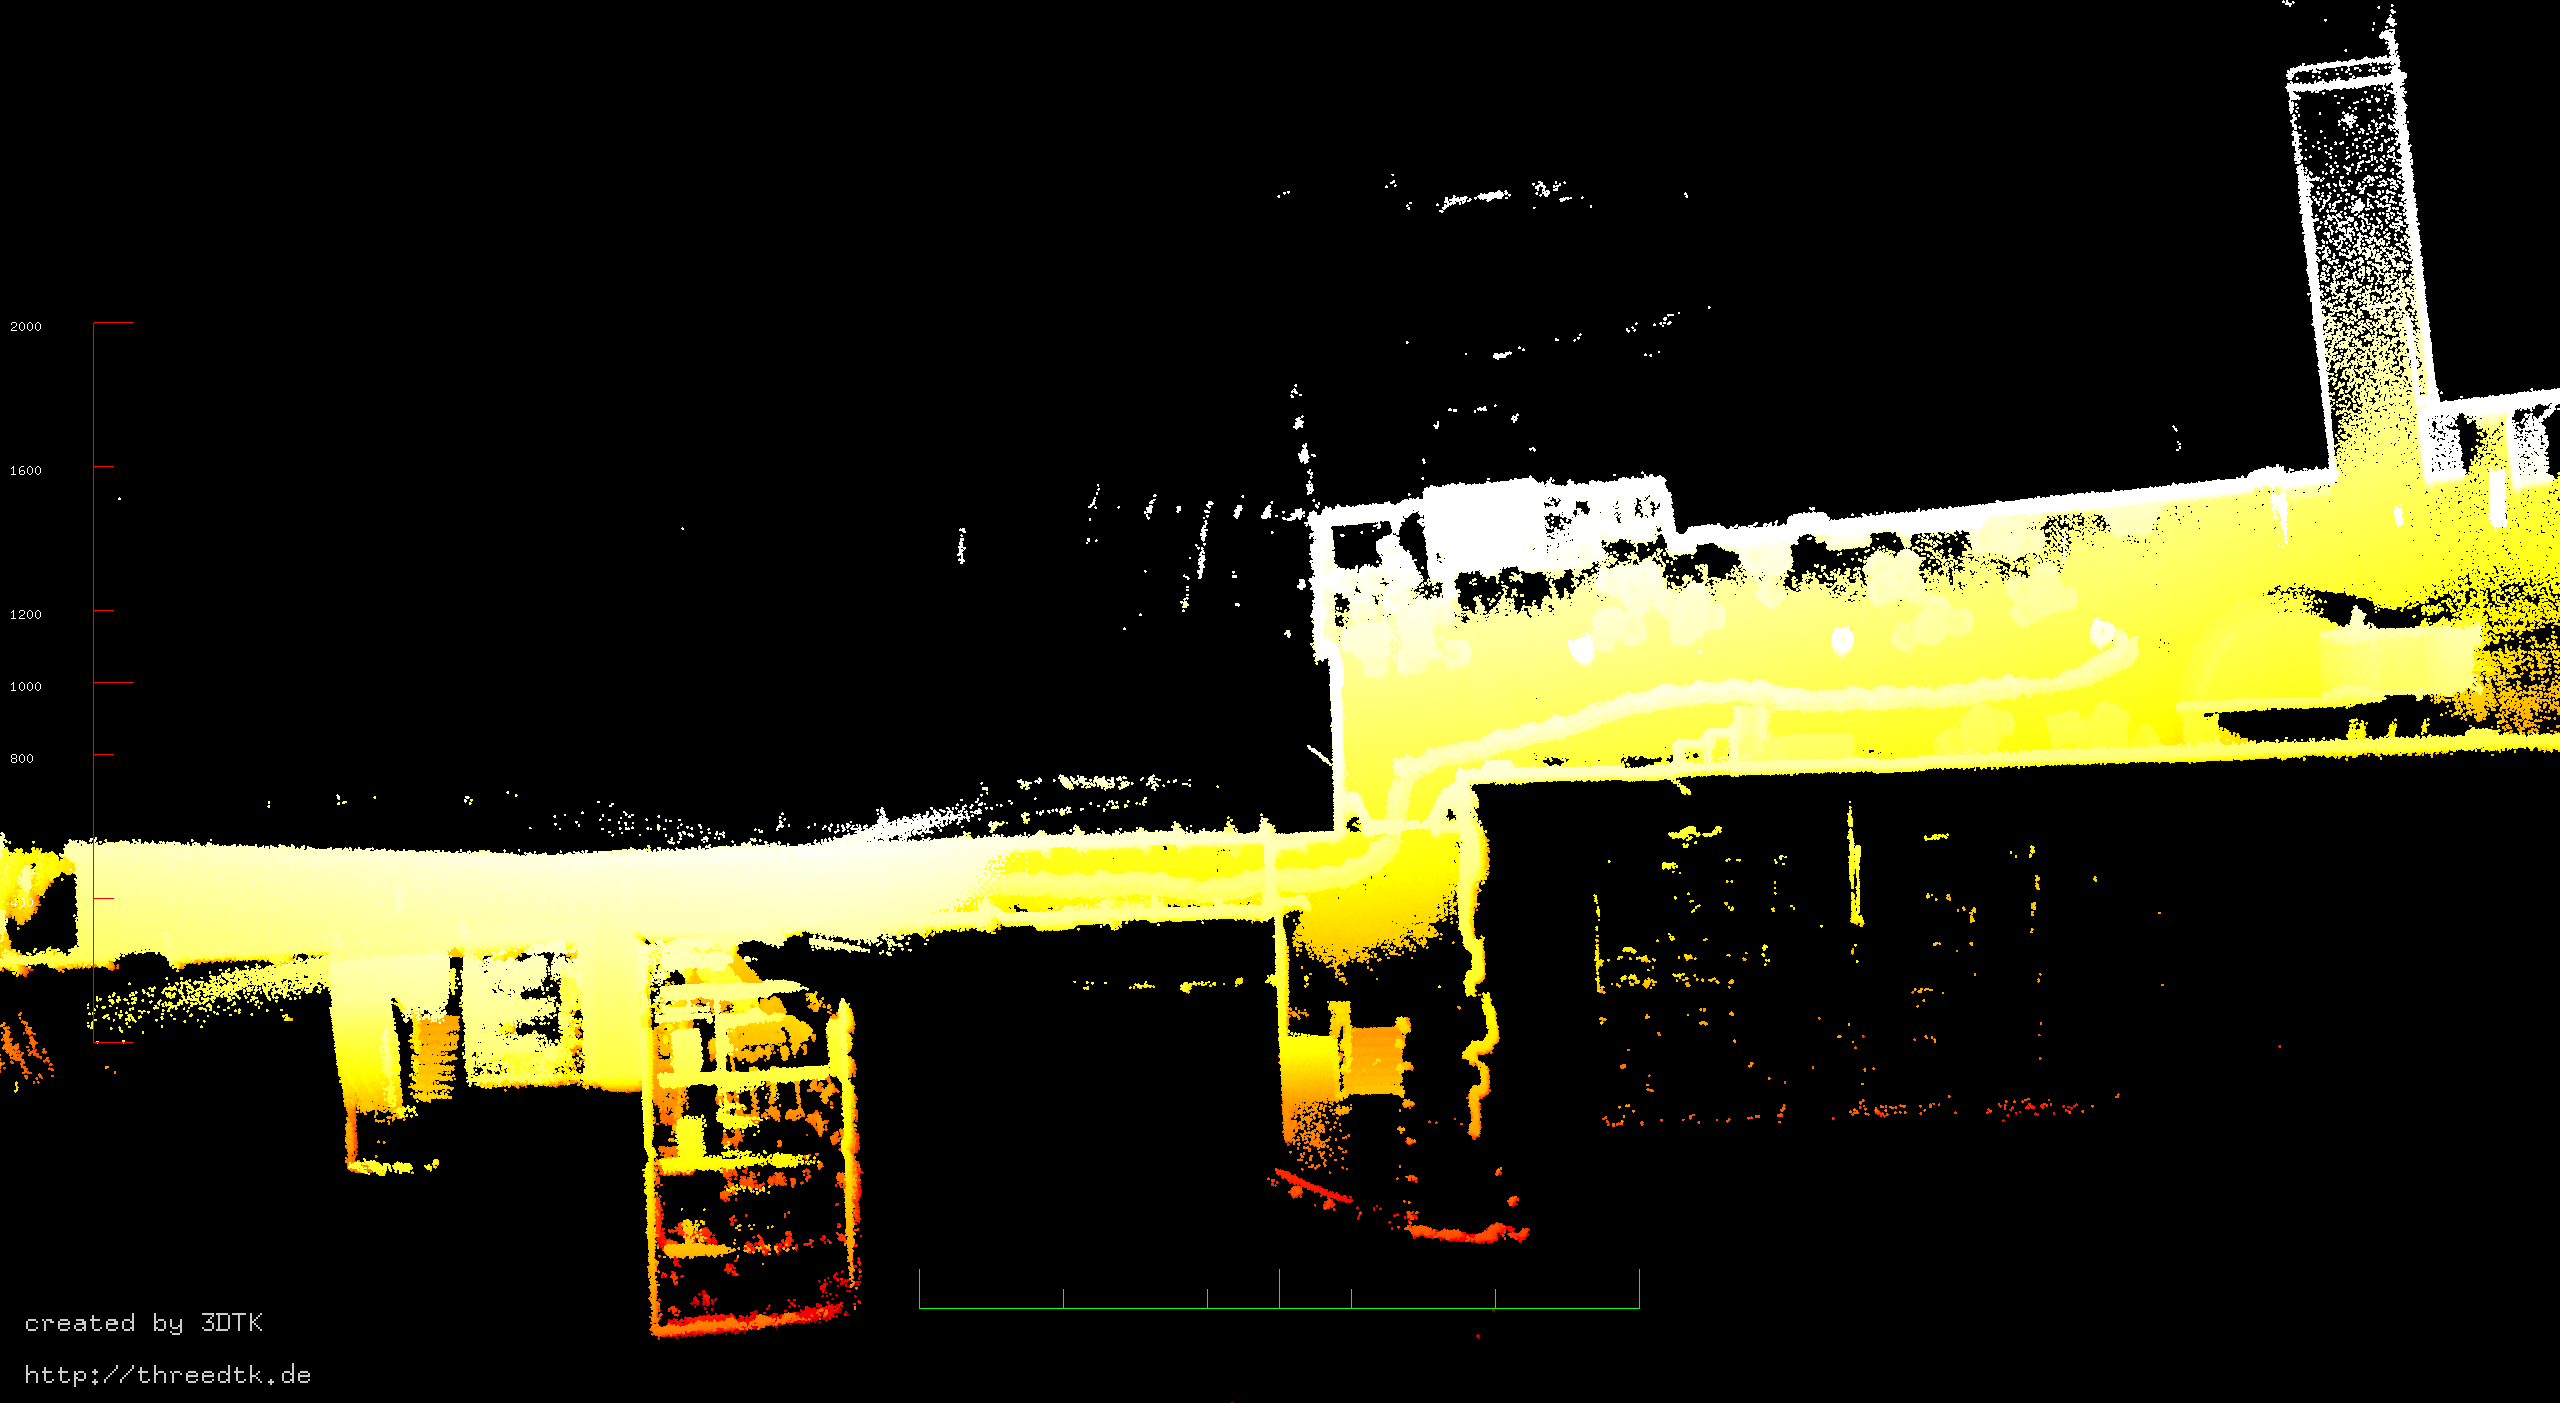
\includegraphics[width=\textwidth]{pics/eagle_view/act_livo_to.png}
        \caption{Actuated FAST-LIVO2}
        \label{fig:act_livo_top}
\end{subfigure}\vspace{2mm}
\begin{subfigure}{0.492\columnwidth}
        \centering
        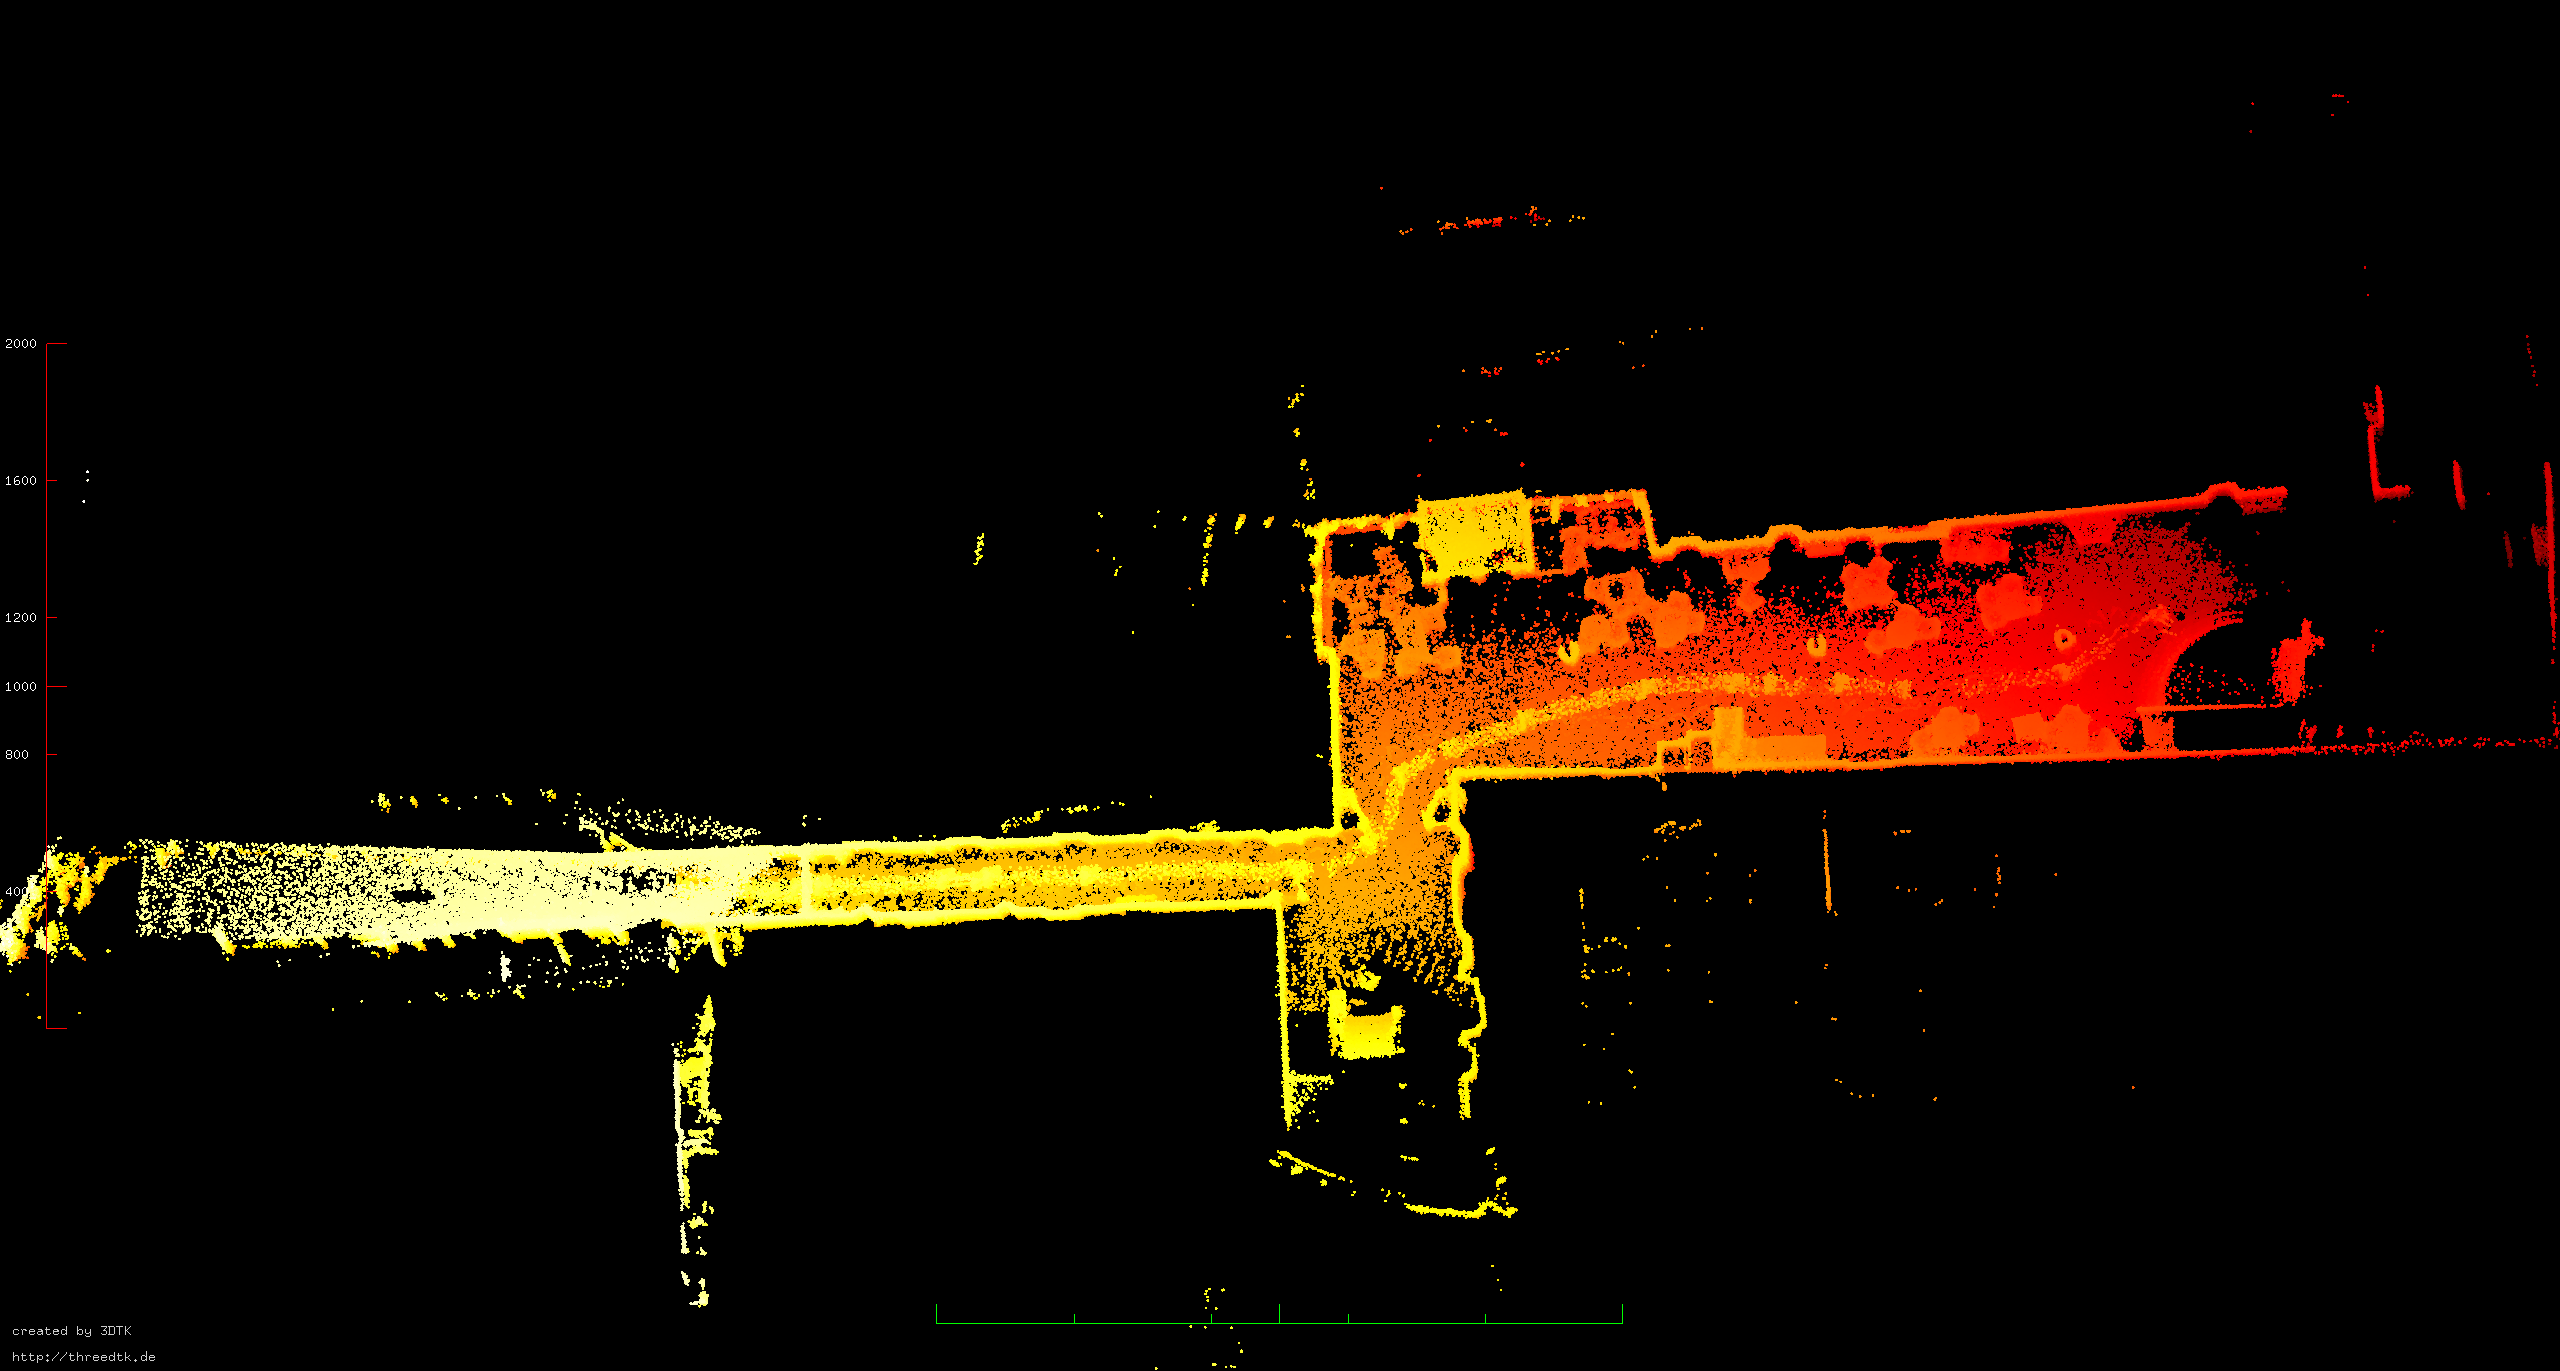
\includegraphics[width=\textwidth]{pics/eagle_view/act_lio_top.png}
        \caption{Actuated FAST-LIO2}
        \label{fig:act_fast_lio_top}\end{subfigure}
\hfill
\begin{subfigure}{0.492\columnwidth}
        \centering
        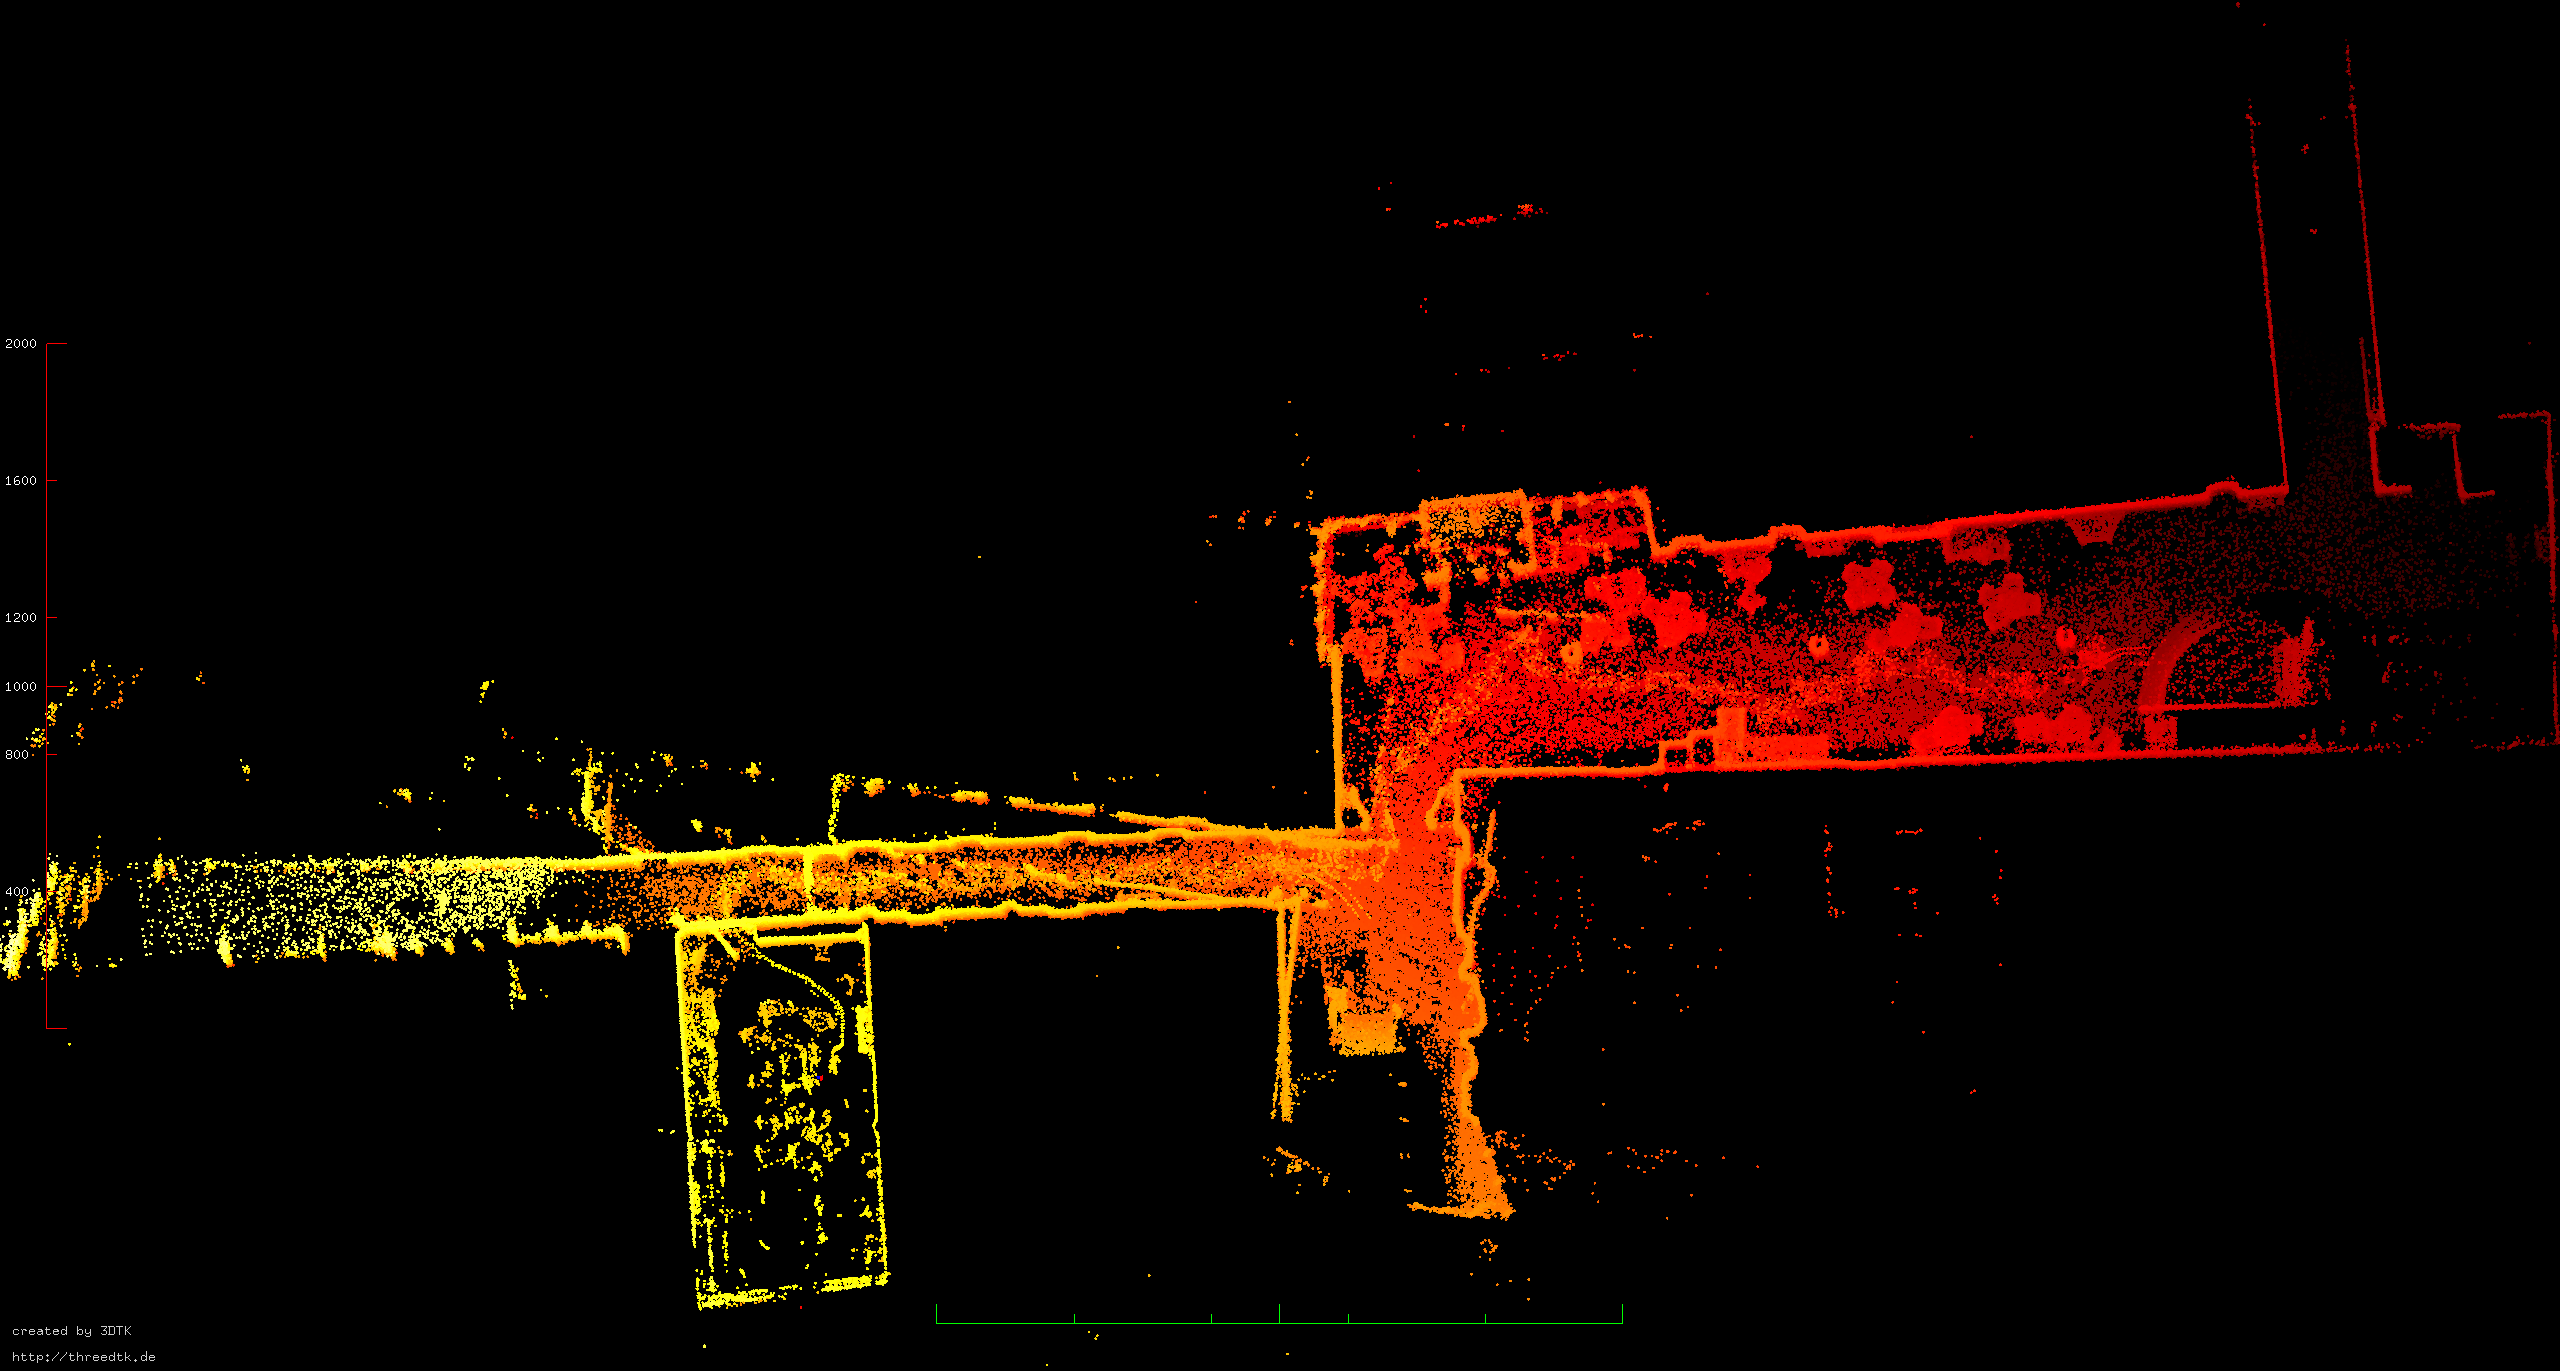
\includegraphics[width=\textwidth]{pics/eagle_view/non_lio_top.png}
        \caption{Non-actuated FAST-LIO2}
        \label{fig:non_act_fast_lio_top}
\end{subfigure}
\caption{Bird's-eye view of a cross section of resulting point-clouds (color indicates height where red means higher).}\vspace{-1mm}
\end{figure}

The error metric used was the point-cloud root mean square error (RMSE).
\begin{equation}
    RMSE = \sqrt{\frac{1}{N} \sum_{i=1}^{N} |p_i - q_i|^2}
\end{equation}
where \( p_i \) and \( q_i \) are the corresponding points in the model and data point-clouds, and \( N \) is the number of corresponding points. 
The RMSE measures the average distance between corresponding points in the two point clouds, providing an indication of the mapping accuracy.


\section{Drift and Bending}
The LIO algorithms exhibited small drift and bending over time, which is particularly noticeable in Fig.~\ref{fig:bending}. 
We were unable to obtain a satisfactory map using DLIO from the non-actuated sphere as shown in Fig.~\ref{fig:dlio_drift}.
Furthermore, sometimes the algorithms drifted without recovering after a fast motion, as shown in Fig.~\ref{fig:lio_drift}. 
We attribute this to the underlying motion models used in the LIO algorithms, which were designed for more conventional systems.

\begin{figure}[h]
\centering
\begin{subfigure}{0.49\columnwidth}
    \centering
    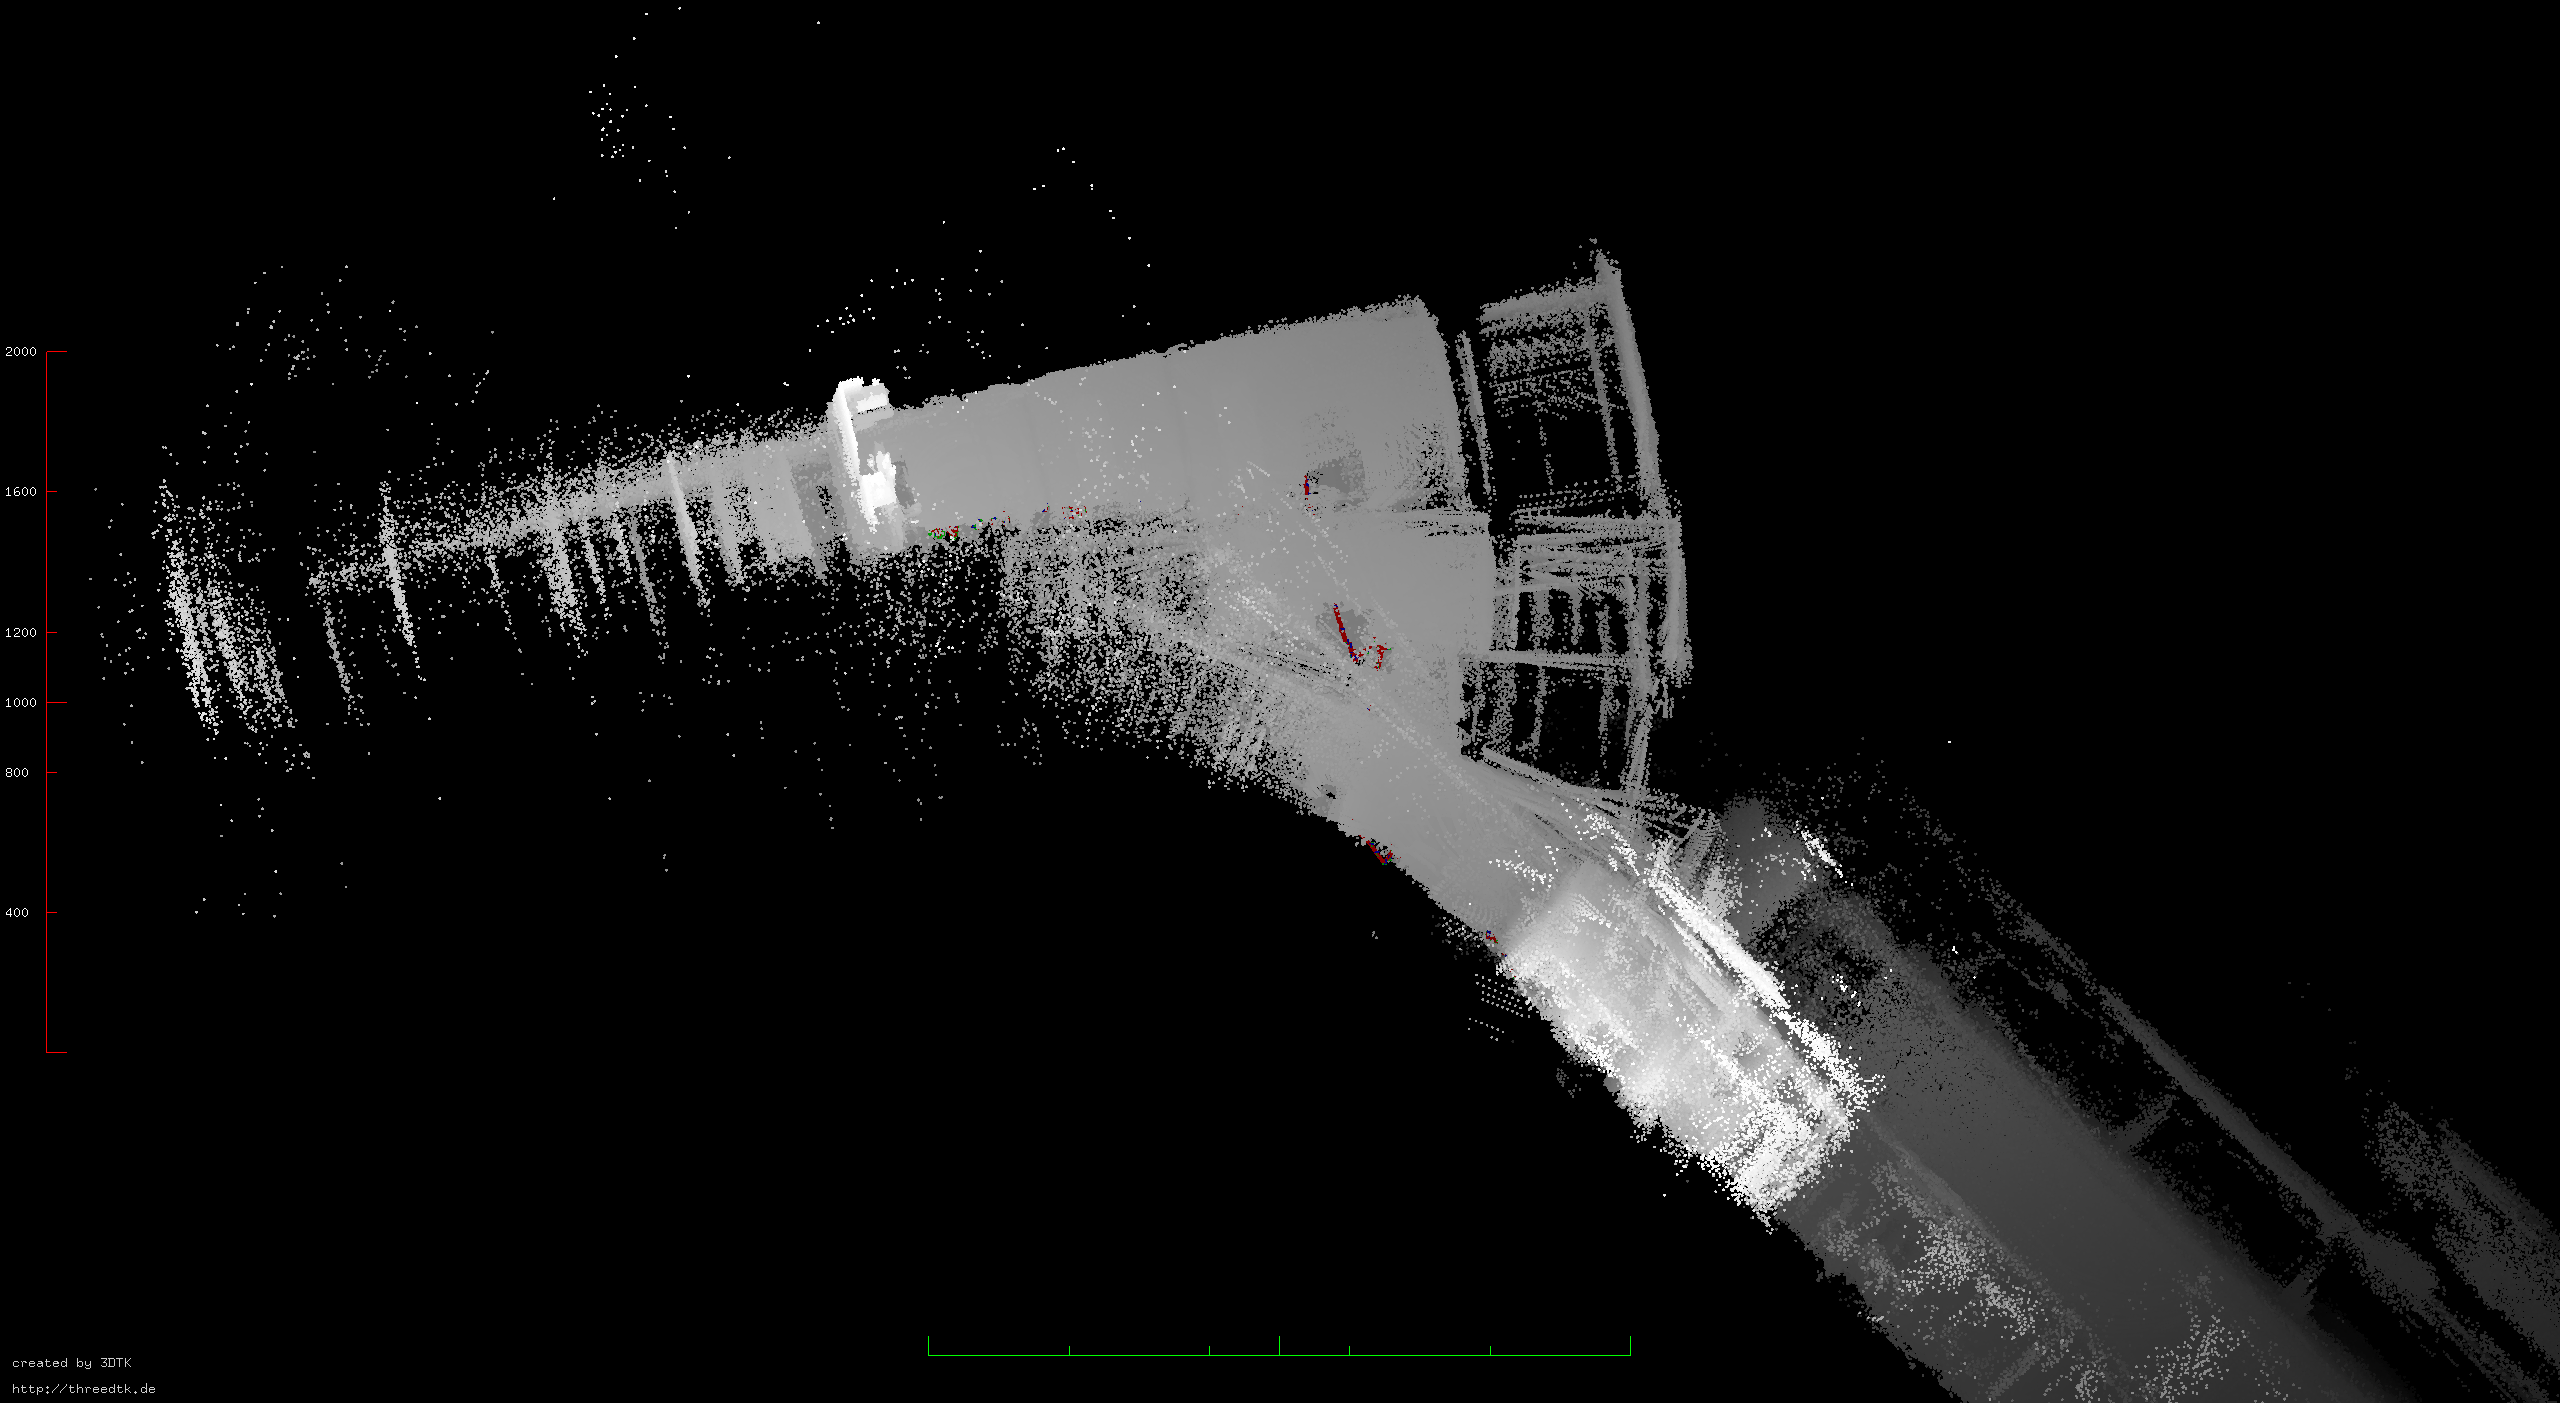
\includegraphics[width=\textwidth]{pics/drifts_bending/dlio_drift.png}
    \caption{Side view of DLIO point-cloud showing severe drift}\label{fig:dlio_drift}
\end{subfigure}
\begin{subfigure}{0.49\columnwidth}
    \centering
    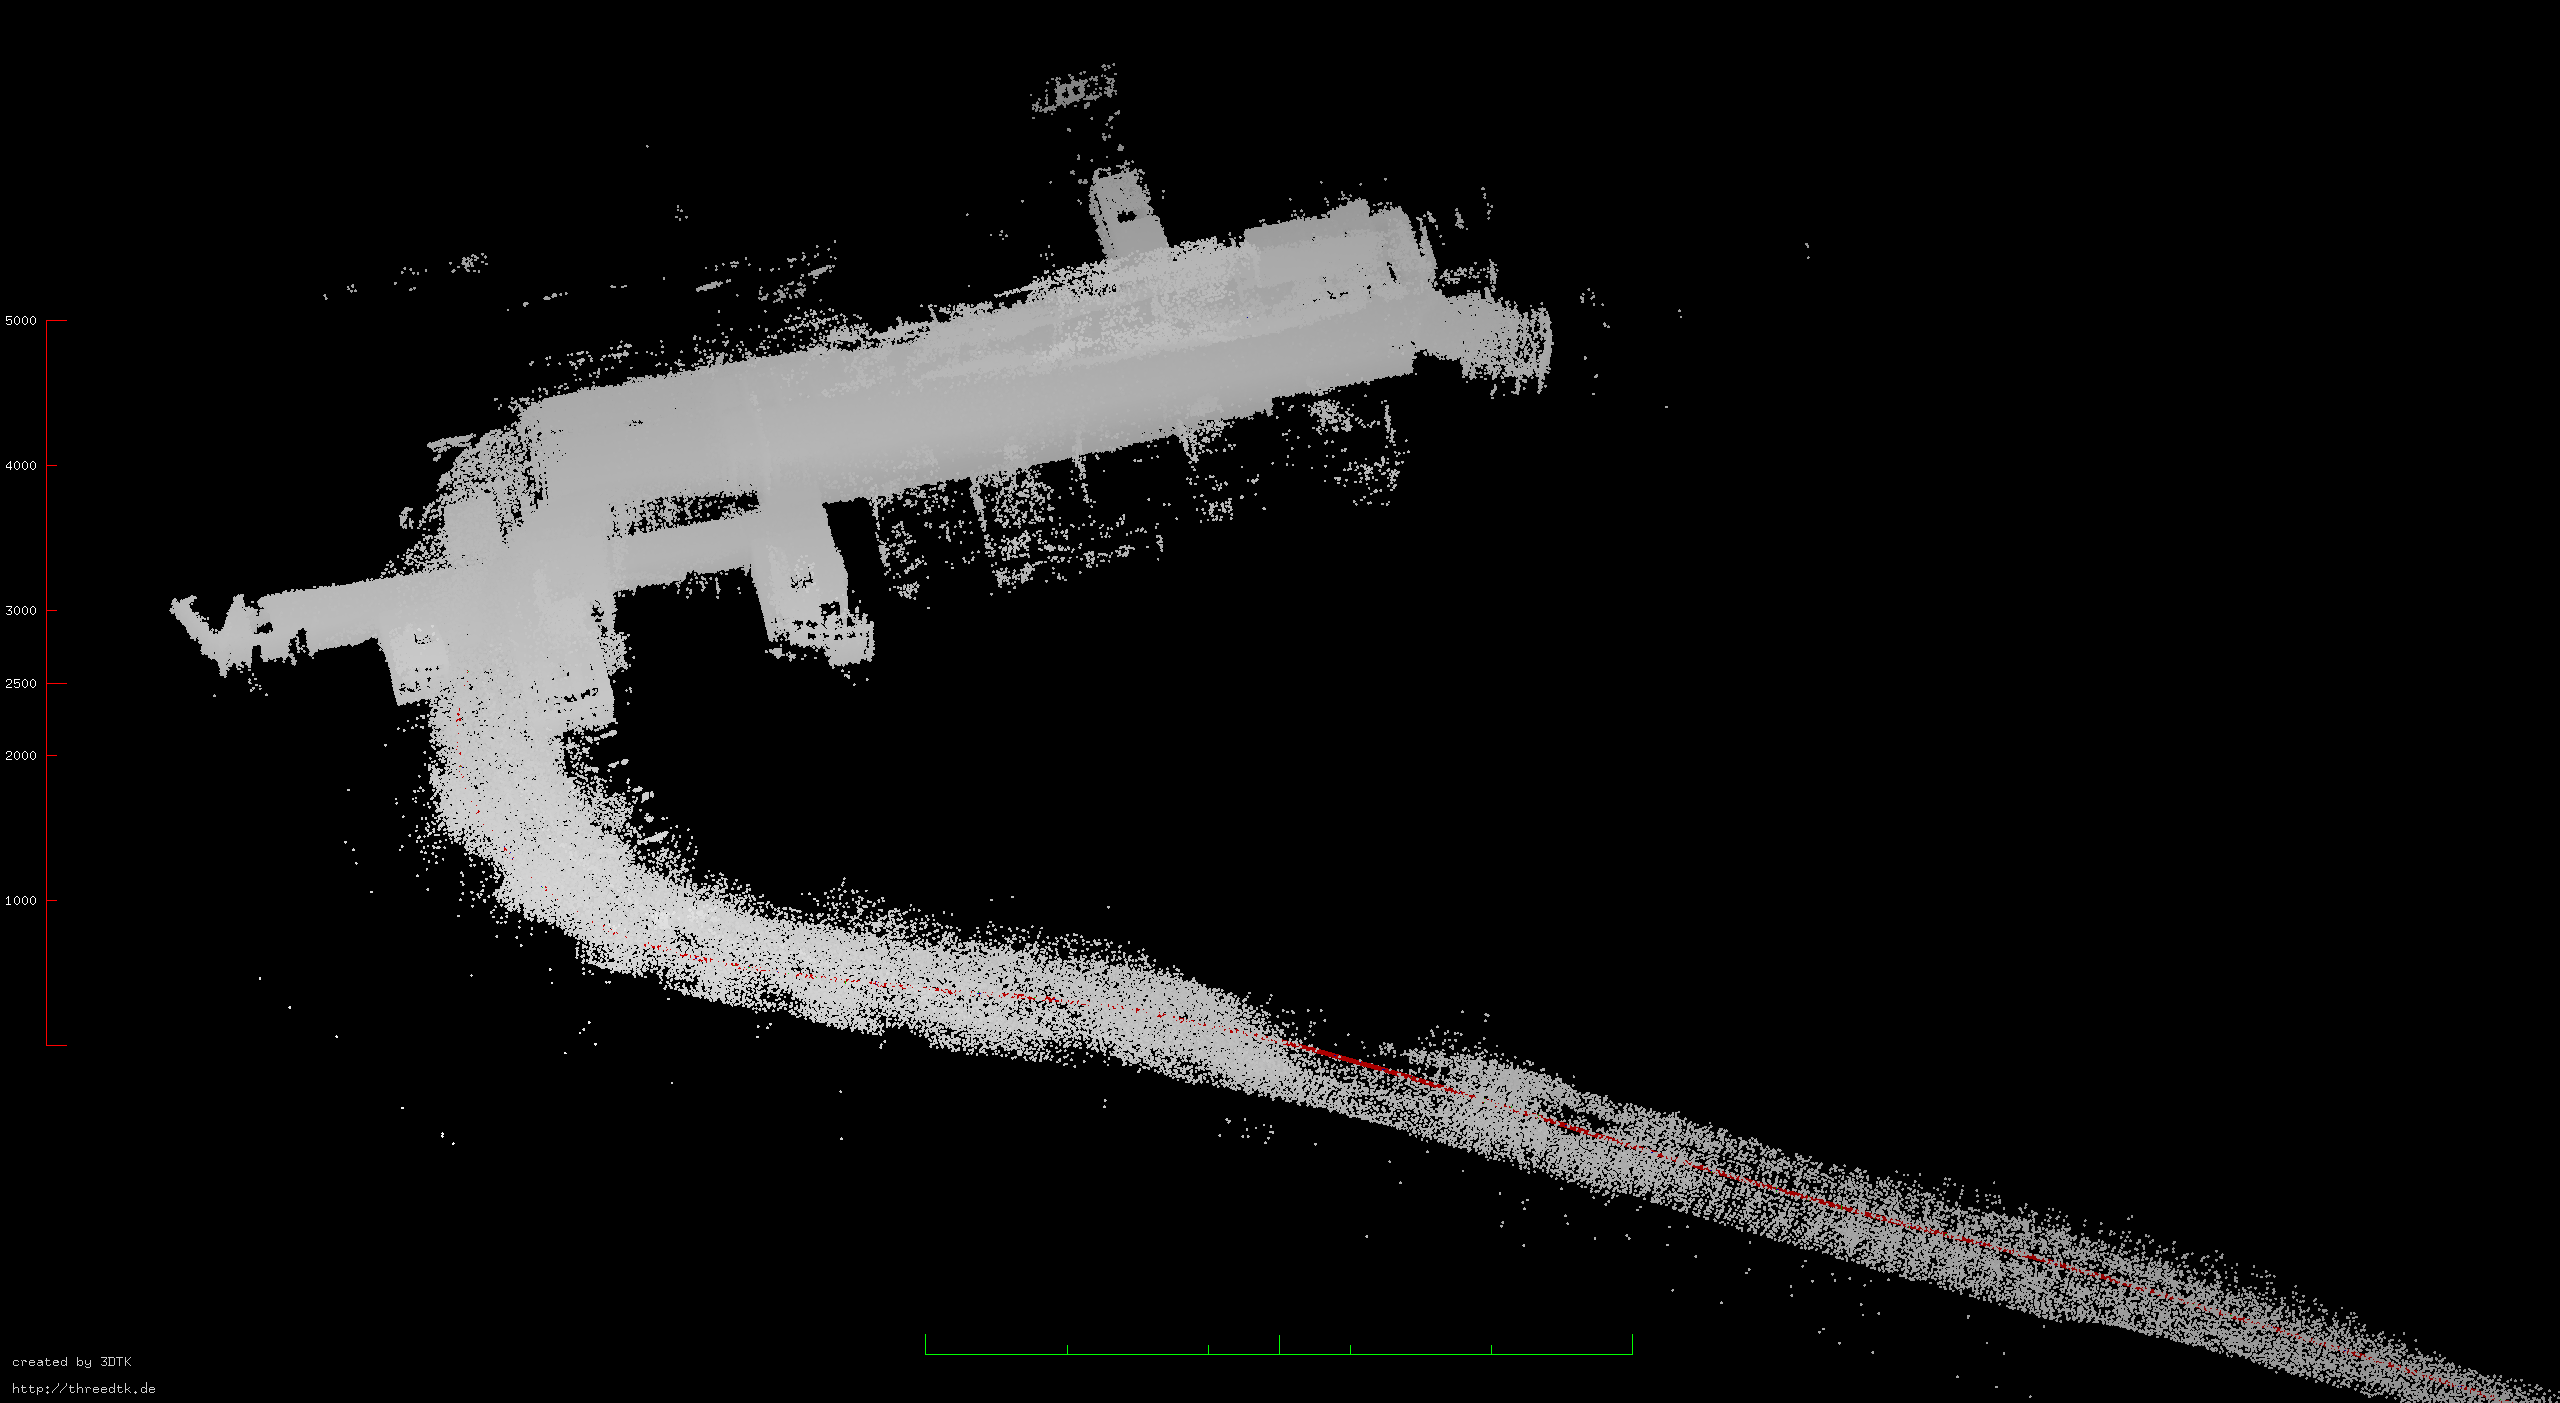
\includegraphics[width=\textwidth]{pics/drifts_bending/lio_drifts.png}
    \caption{Bird's-eye view of FAST-LIO2 point-cloud}\label{fig:lio_drift}
\end{subfigure}
\caption{Example failed cases from the non-actuated sphere where the LIO algorithm could not recover due to fast angular motion.
This results in huge drift and inconsistent mapping.}\vspace{-3mm}
\label{fig:drift}
\end{figure}
\begin{figure}[h]
\centering
\begin{subfigure}{0.49\columnwidth}
    \centering
    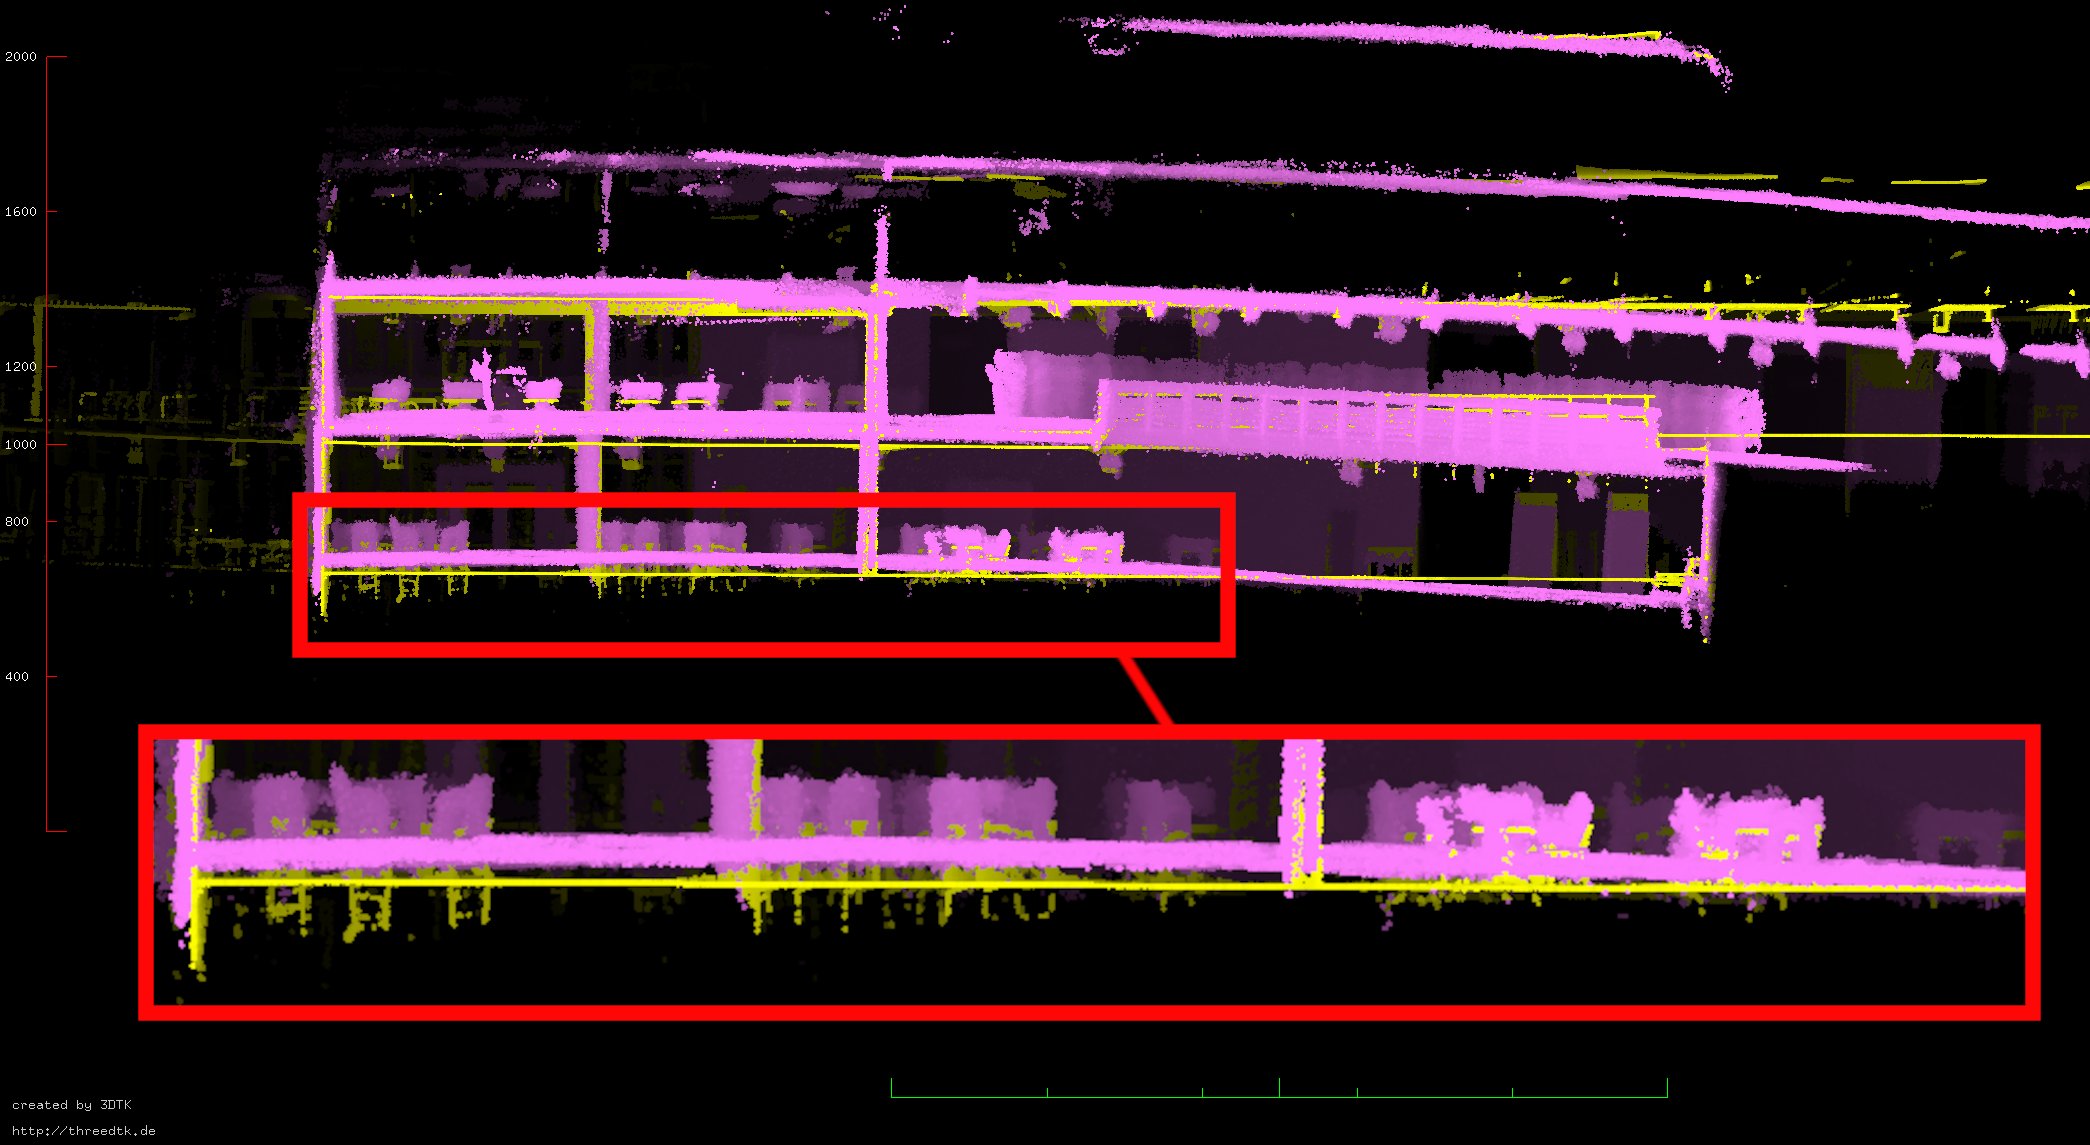
\includegraphics[width=\textwidth]{pics/drifts_bending/dlio_bending.png}
    \caption{DLIO point-cloud}\label{fig:dlio_bending}
    \end{subfigure}
\begin{subfigure}{0.49\columnwidth}
    \centering
    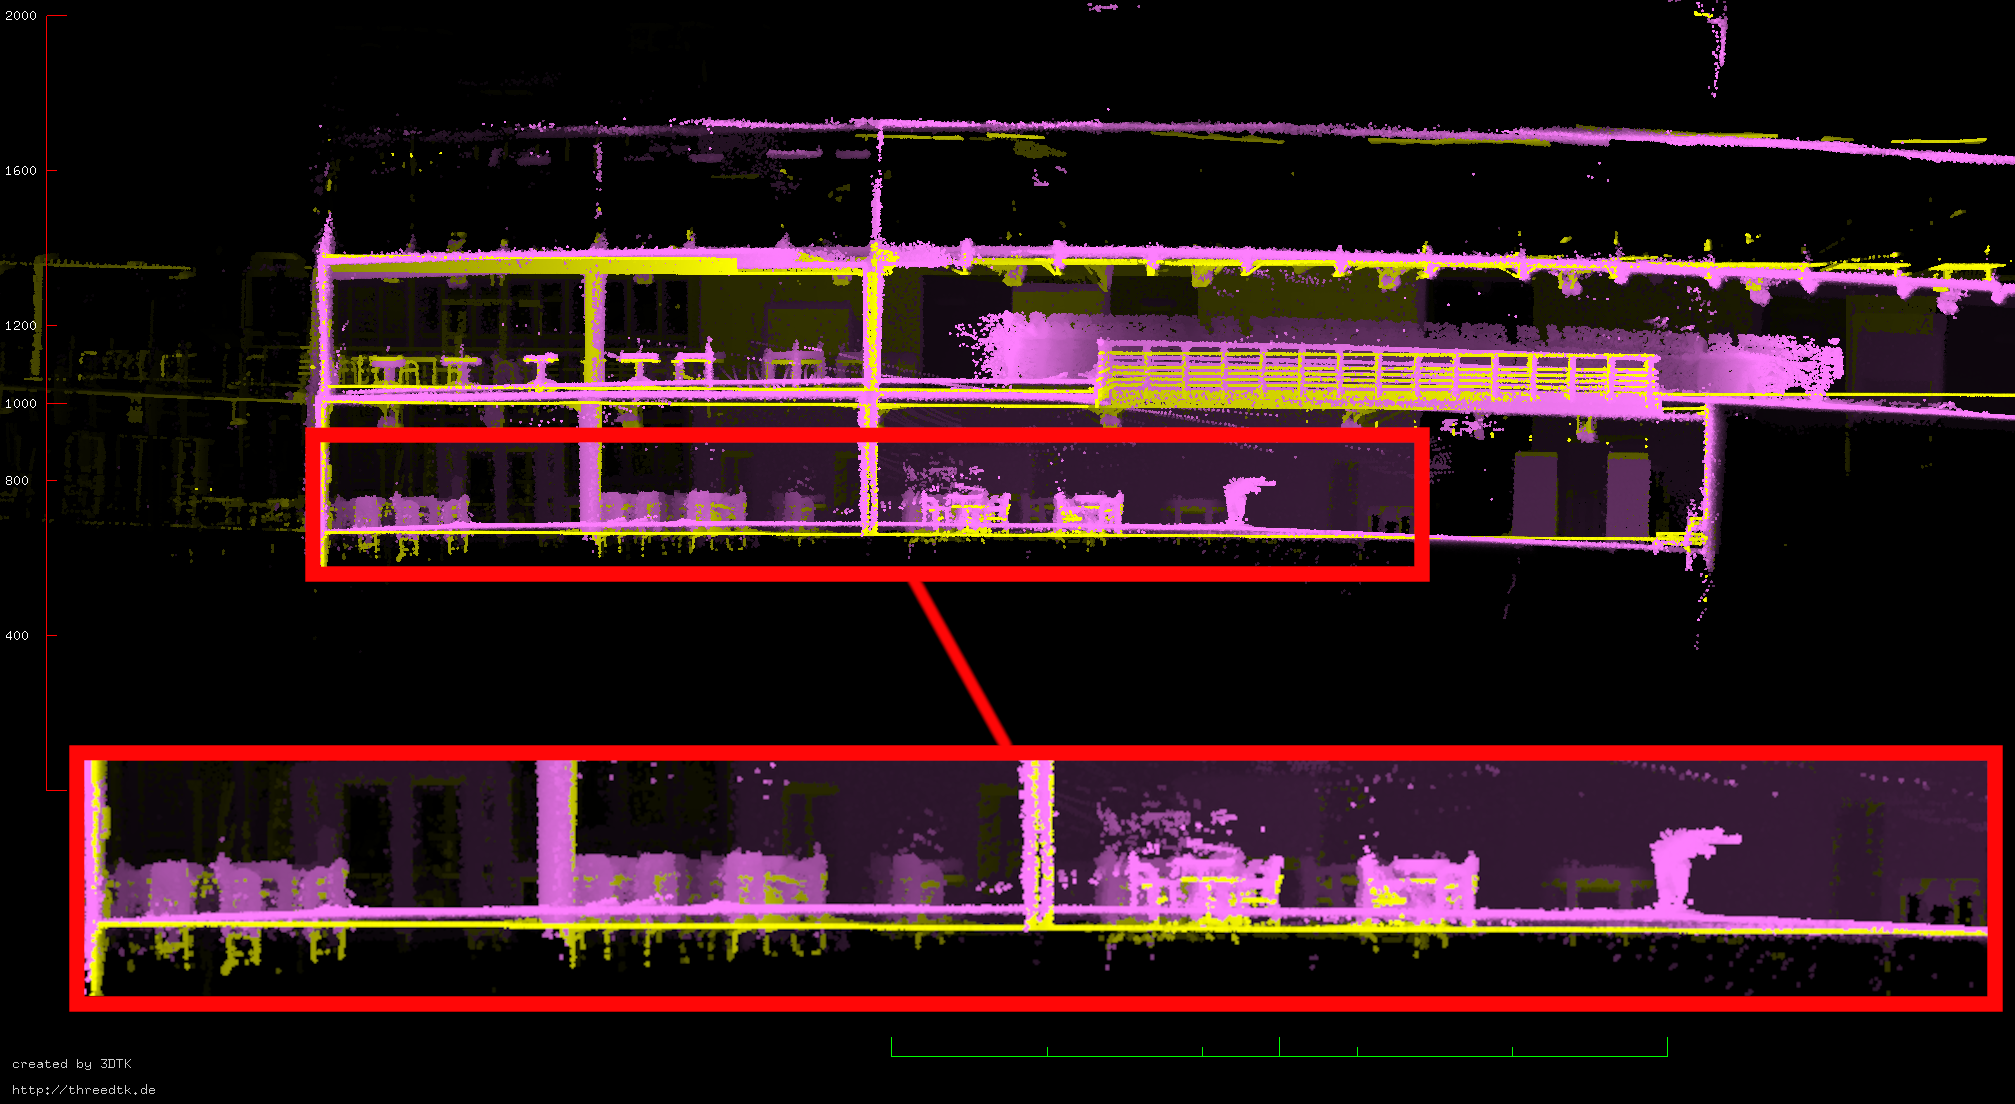
\includegraphics[width=\textwidth]{pics/drifts_bending/livo_actuated_bending.png}
    \caption{FAST-LIVO2 point-cloud}\label{fig:livo_bending}
\end{subfigure}
\caption{Cross section comparison. 
Yellow: Ground truth, Magenta: Mentioned algorithm.
The red boxes indicate noticeable bending of the ground plane.}\vspace{-1mm}
\label{fig:bending}
\end{figure}

\clearpage
\section{Mapping Accuracy}
We evaluate the point-cloud error for each mapping run using the three SLAM algorithms. 
Table~\ref{tab:point_cloud_error} summarizes the results.
The statistical analysis reveals significant differences in mapping performance across configurations. 
The non-actuated sphere with FAST-LIO2 achieved the lowest mean error (\SI{9.60}{\centi\meter}) and RMSE (\SI{13.09}{\centi\meter}), indicating superior accuracy. 
This is unexpected since the motion of the non-actuated sphere is governed by larger rotations around all principal axes and more aggressive dynamics.
We attribute the overall better mapping performance of the non-actuated sphere to its smaller shell radius and missing locomotion mechanism structure.
Thus, we were able to place the laser scanner closer to the center of the sphere.
%However, the actuated sphere generally captured more data points, with DLIO collecting 88.01 million points compared to 1.99 million for non-actuated FAST-LIO2. 
%All configurations showed highly significant results (p < 0.001), confirming systematic measurement patterns rather than random noise. 
\clearpage

\begin{sidewaystable}
\centering
\begin{threeparttable}
\caption{Statistical analysis of point-cloud mapping accuracy.}
\label{tab:point_cloud_error}
\begin{tabular}{l|cc|cc|cc}
\toprule
\textbf{Metric} & \multicolumn{2}{c|}{\textbf{FAST-LIO2}} & \multicolumn{2}{c|}{\textbf{FAST-LIVO2(LIO-Mode)}} & \multicolumn{2}{c}{\textbf{DLIO}} \\
& \textbf{Non-act.} & \textbf{Act.} & \textbf{Non-act.} & \textbf{Act.} & \textbf{Non-act.} & \textbf{Act.} \\
\midrule
\textbf{Points ($\times 10^6$)} & 1.99 & 4.43 & 16.36 & 46.39 & - & 88.01 \\
\textbf{Mean$^1$ (cm)} & \bf{9.60} & 10.73 & \bf{12.05} & 12.93 & - & \bf{13.71} \\
\textbf{Std Dev (cm)} & 8.91 & 9.96 & 11.33 & 12.58 & - & 13.26 \\
\textbf{RMSE$^1$ (cm)} & \bf{13.09} & 14.64 & \bf{16.54} & 18.04 & - & \bf{19.08} \\
\textbf{P95$^2$ (cm)} & \bf{26.76} & 30.47 & \bf{37.33} & 41.04 & - & \bf{42.36} \\
\textbf{P90$^2$ (cm)} & \bf{18.58} & 22.57 & \bf{26.48} & 31.63 & - & \bf{34.70} \\
\bottomrule
\end{tabular}
\begin{tablenotes}
    \item (-) denotes that the algorithm failed.
    \item[1] Refers to the point-to-point errors to ground truth.
    \item[2] Refers to the percent of points having point-to-point errors to ground truth smaller than the given value. 
\end{tablenotes}
\end{threeparttable}
\end{sidewaystable}
\clearpage
\begin{figure*}
\centering
% First row - 5 subfigures
\begin{subfigure}{0.45\textwidth}
    \centering
    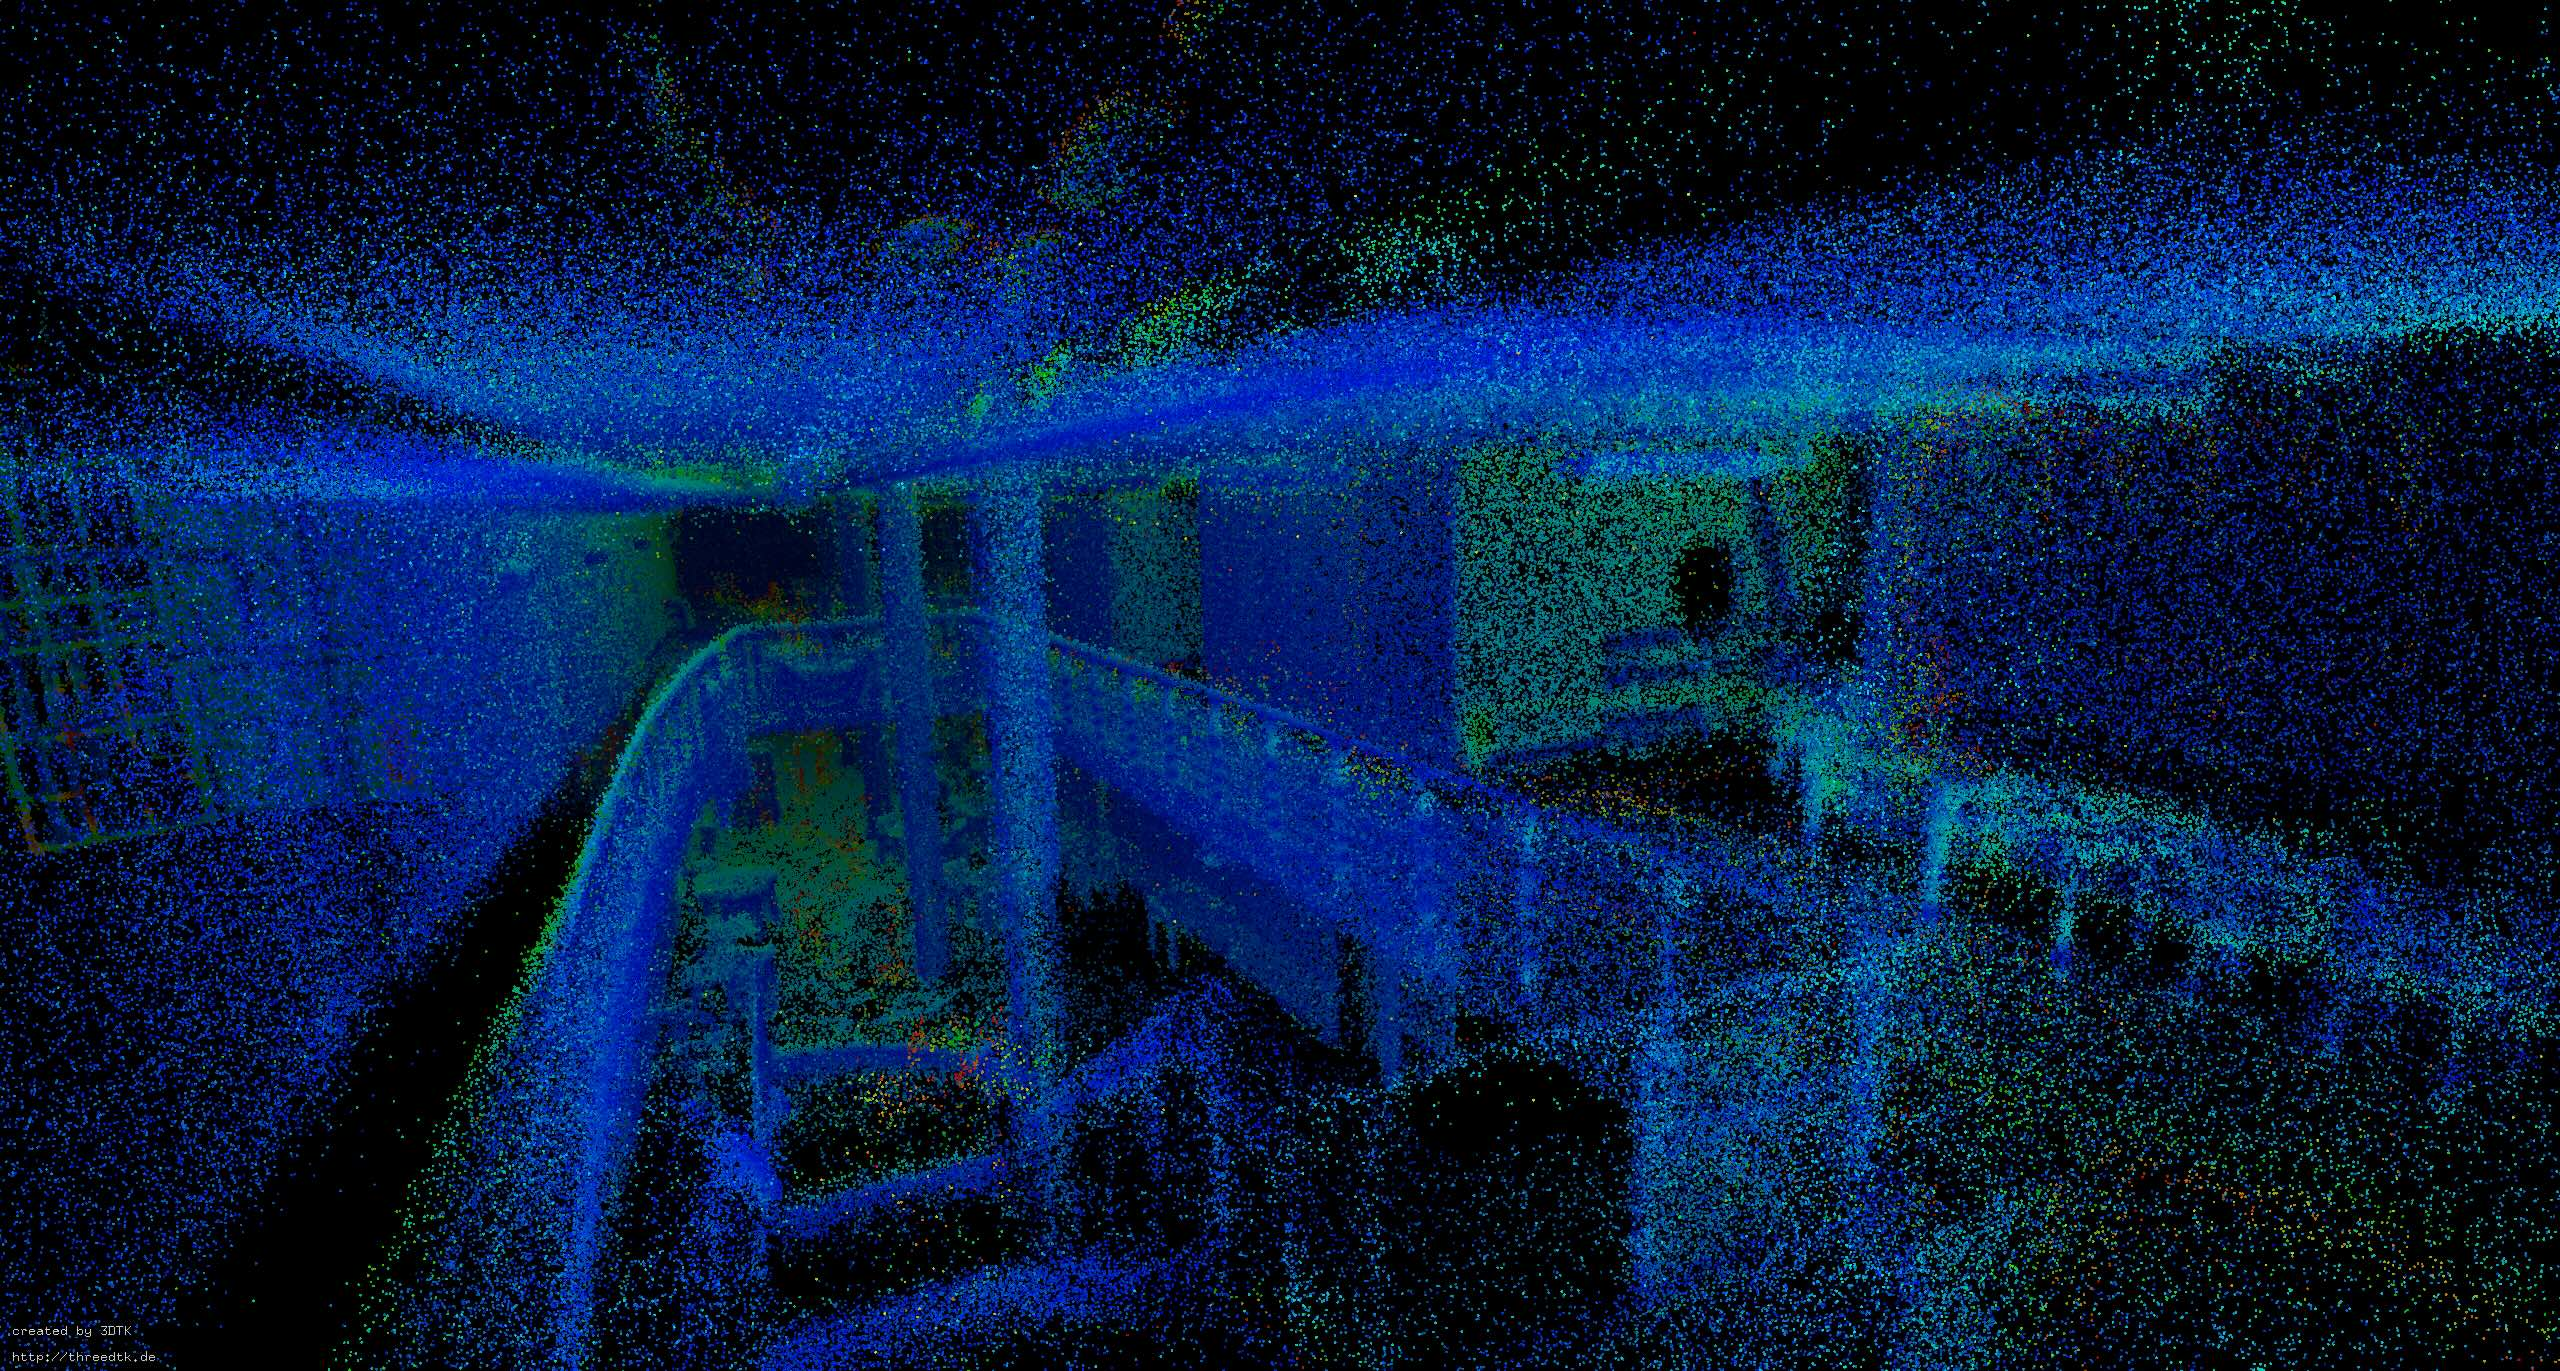
\includegraphics[width=\textwidth]{pics/results_images/non_lio.jpg}
    \label{fig:results_non_lio}
\end{subfigure}
\begin{subfigure}{0.45\textwidth}
    \centering
    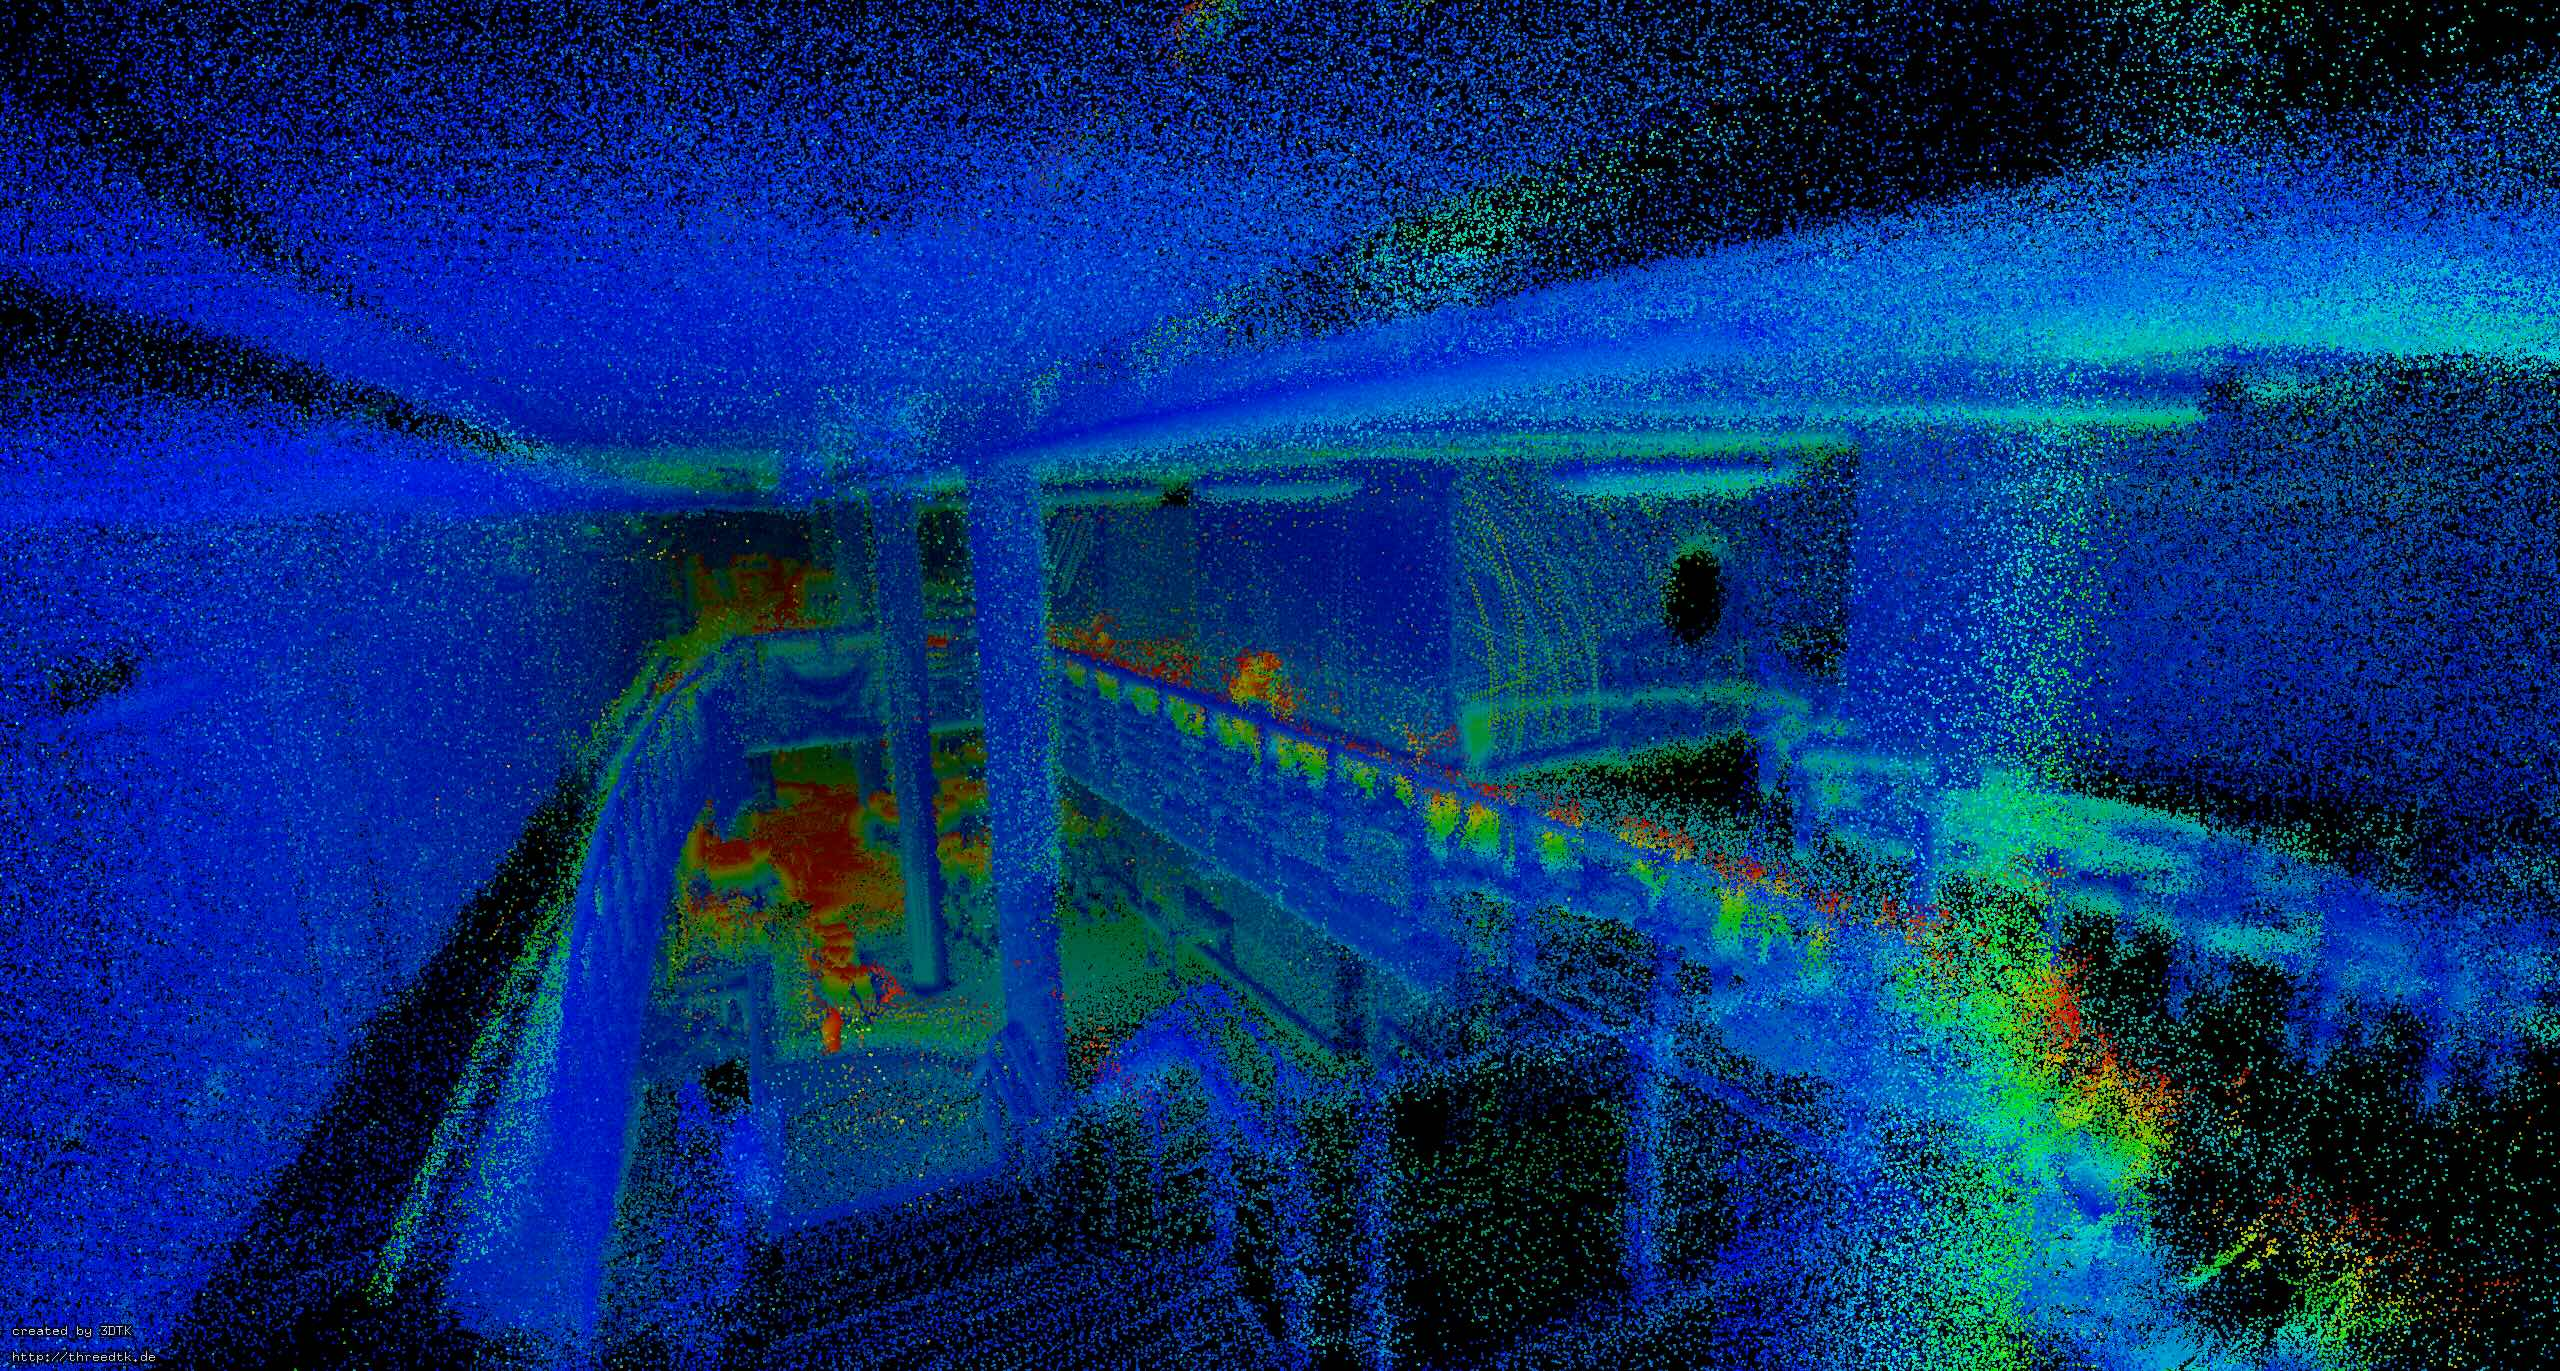
\includegraphics[width=\textwidth]{pics/results_images/non_livo.jpg}
    \label{fig:results_non_livo}
\end{subfigure}

% Second row - 2 subfigures (centered)
\begin{subfigure}{0.45\textwidth}
    \centering
    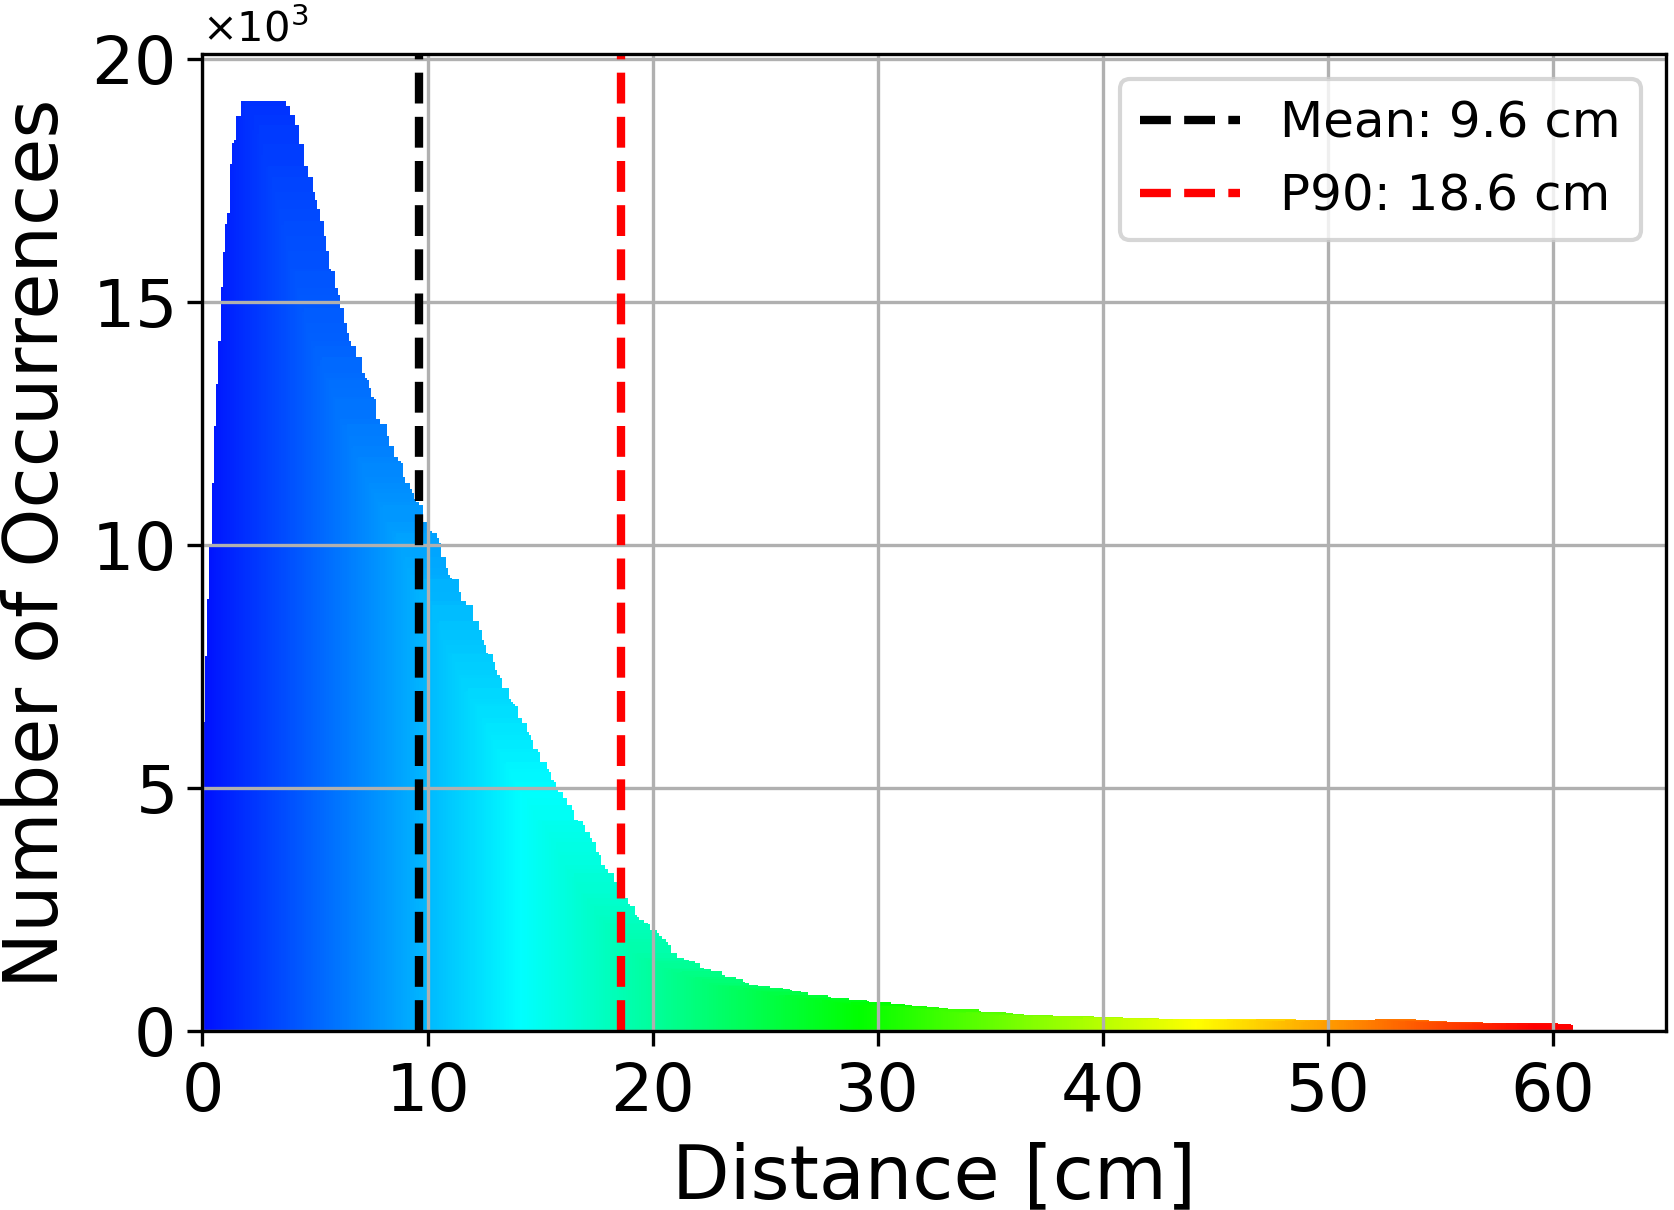
\includegraphics[width=\textwidth]{pics/histogram_results/histogram_cond_non_actuated_lio.png}
    \caption{Non-Act. FAST-LIO2}
    \label{fig:hist_non_lio}
\end{subfigure}
\begin{subfigure}{0.45\textwidth}
    \centering
    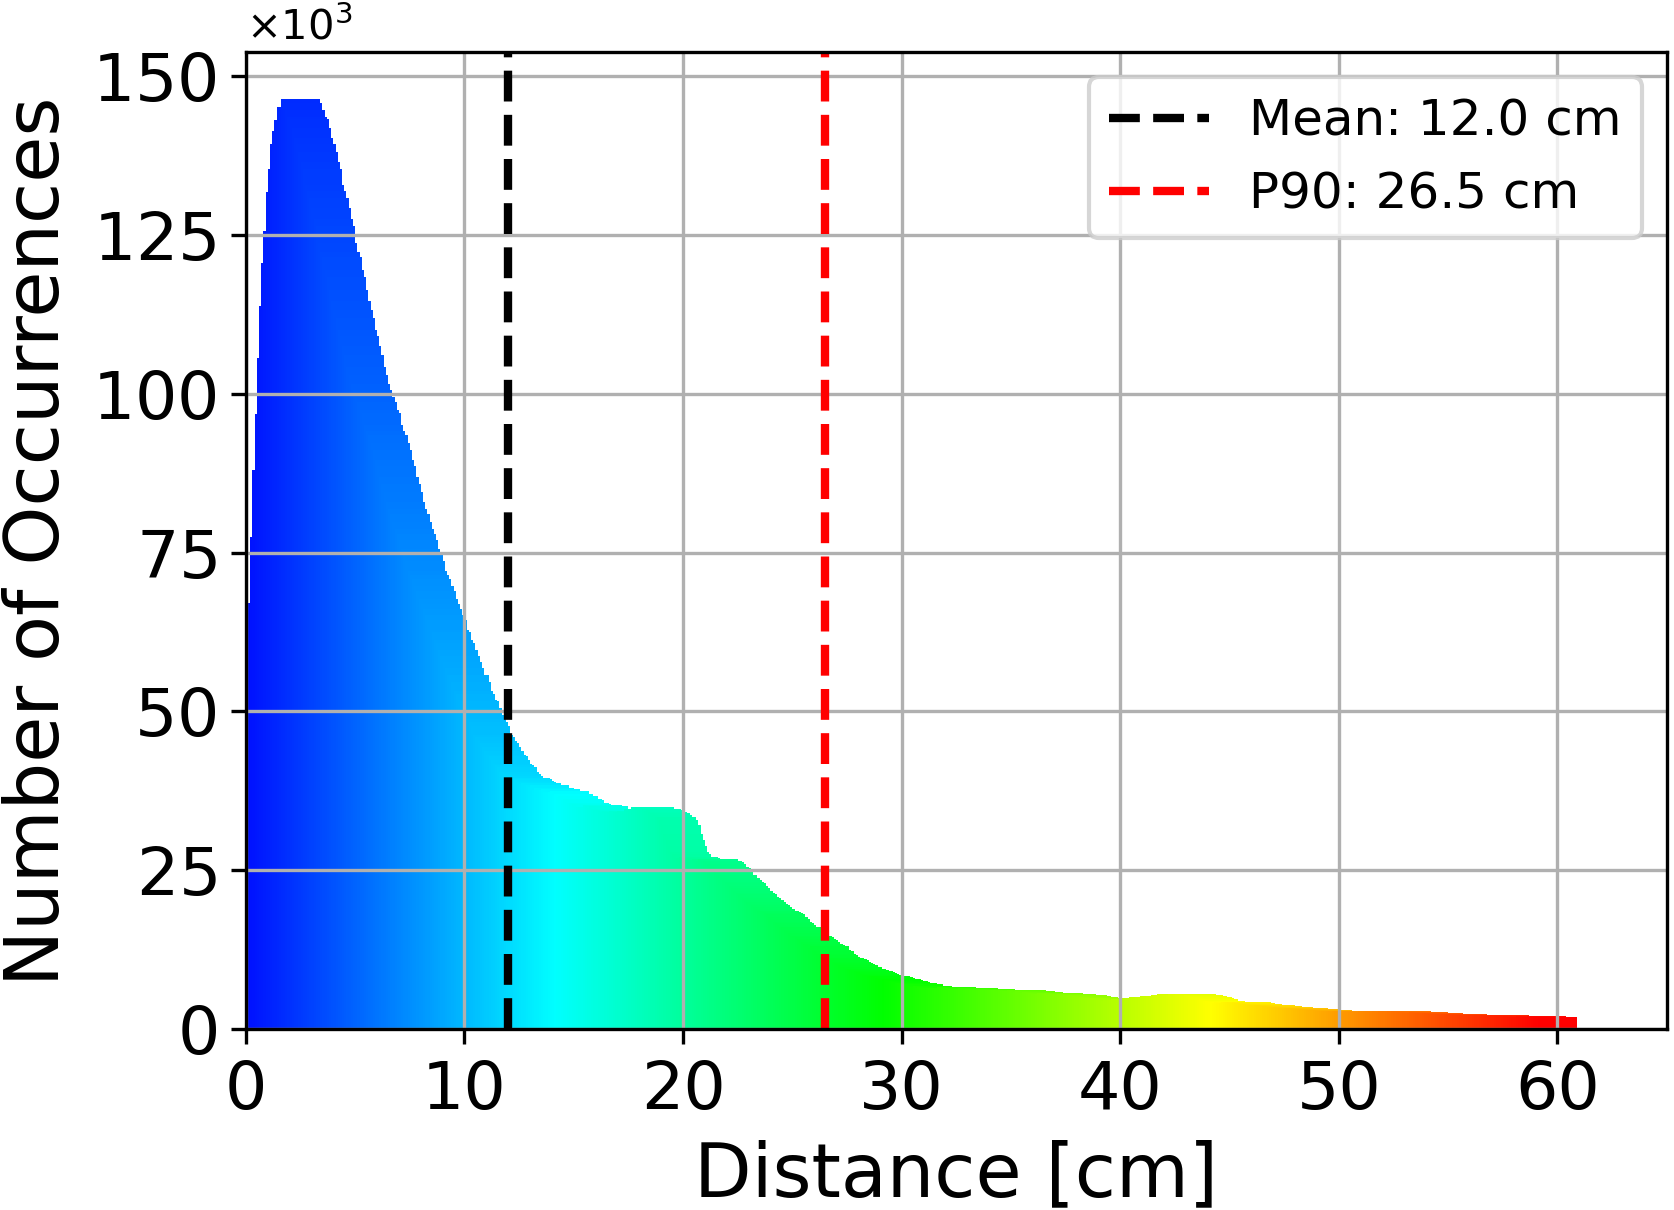
\includegraphics[width=\textwidth]{pics/histogram_results/histogram_cond_non_actuated_livo.png}
    \caption{Non-Act. FAST-LIVO2}
    \label{fig:hist_non_livo}
\end{subfigure}

\begin{subfigure}{0.3\textwidth}
    \centering
    \includegraphics[width=\textwidth]{pics/histogram_results/hsv.png}
    \caption{Color Mapping}
    \label{fig:hsv}
\end{subfigure}
\caption{Point-cloud results and error distribution analysis. A fly through video of the point-clouds is available at \url{https://youtu.be/Ere4UjPg-gk}. 
The first row shows the point-clouds generated by comparing the RIEGL map with each algorithm, while the second row displays the corresponding error distribution Analysis(Part 1).}
\label{fig:combined_results1}
\end{figure*}

\begin{figure*}
    \centering
    %here
\begin{subfigure}{0.4\textwidth}
    \centering
    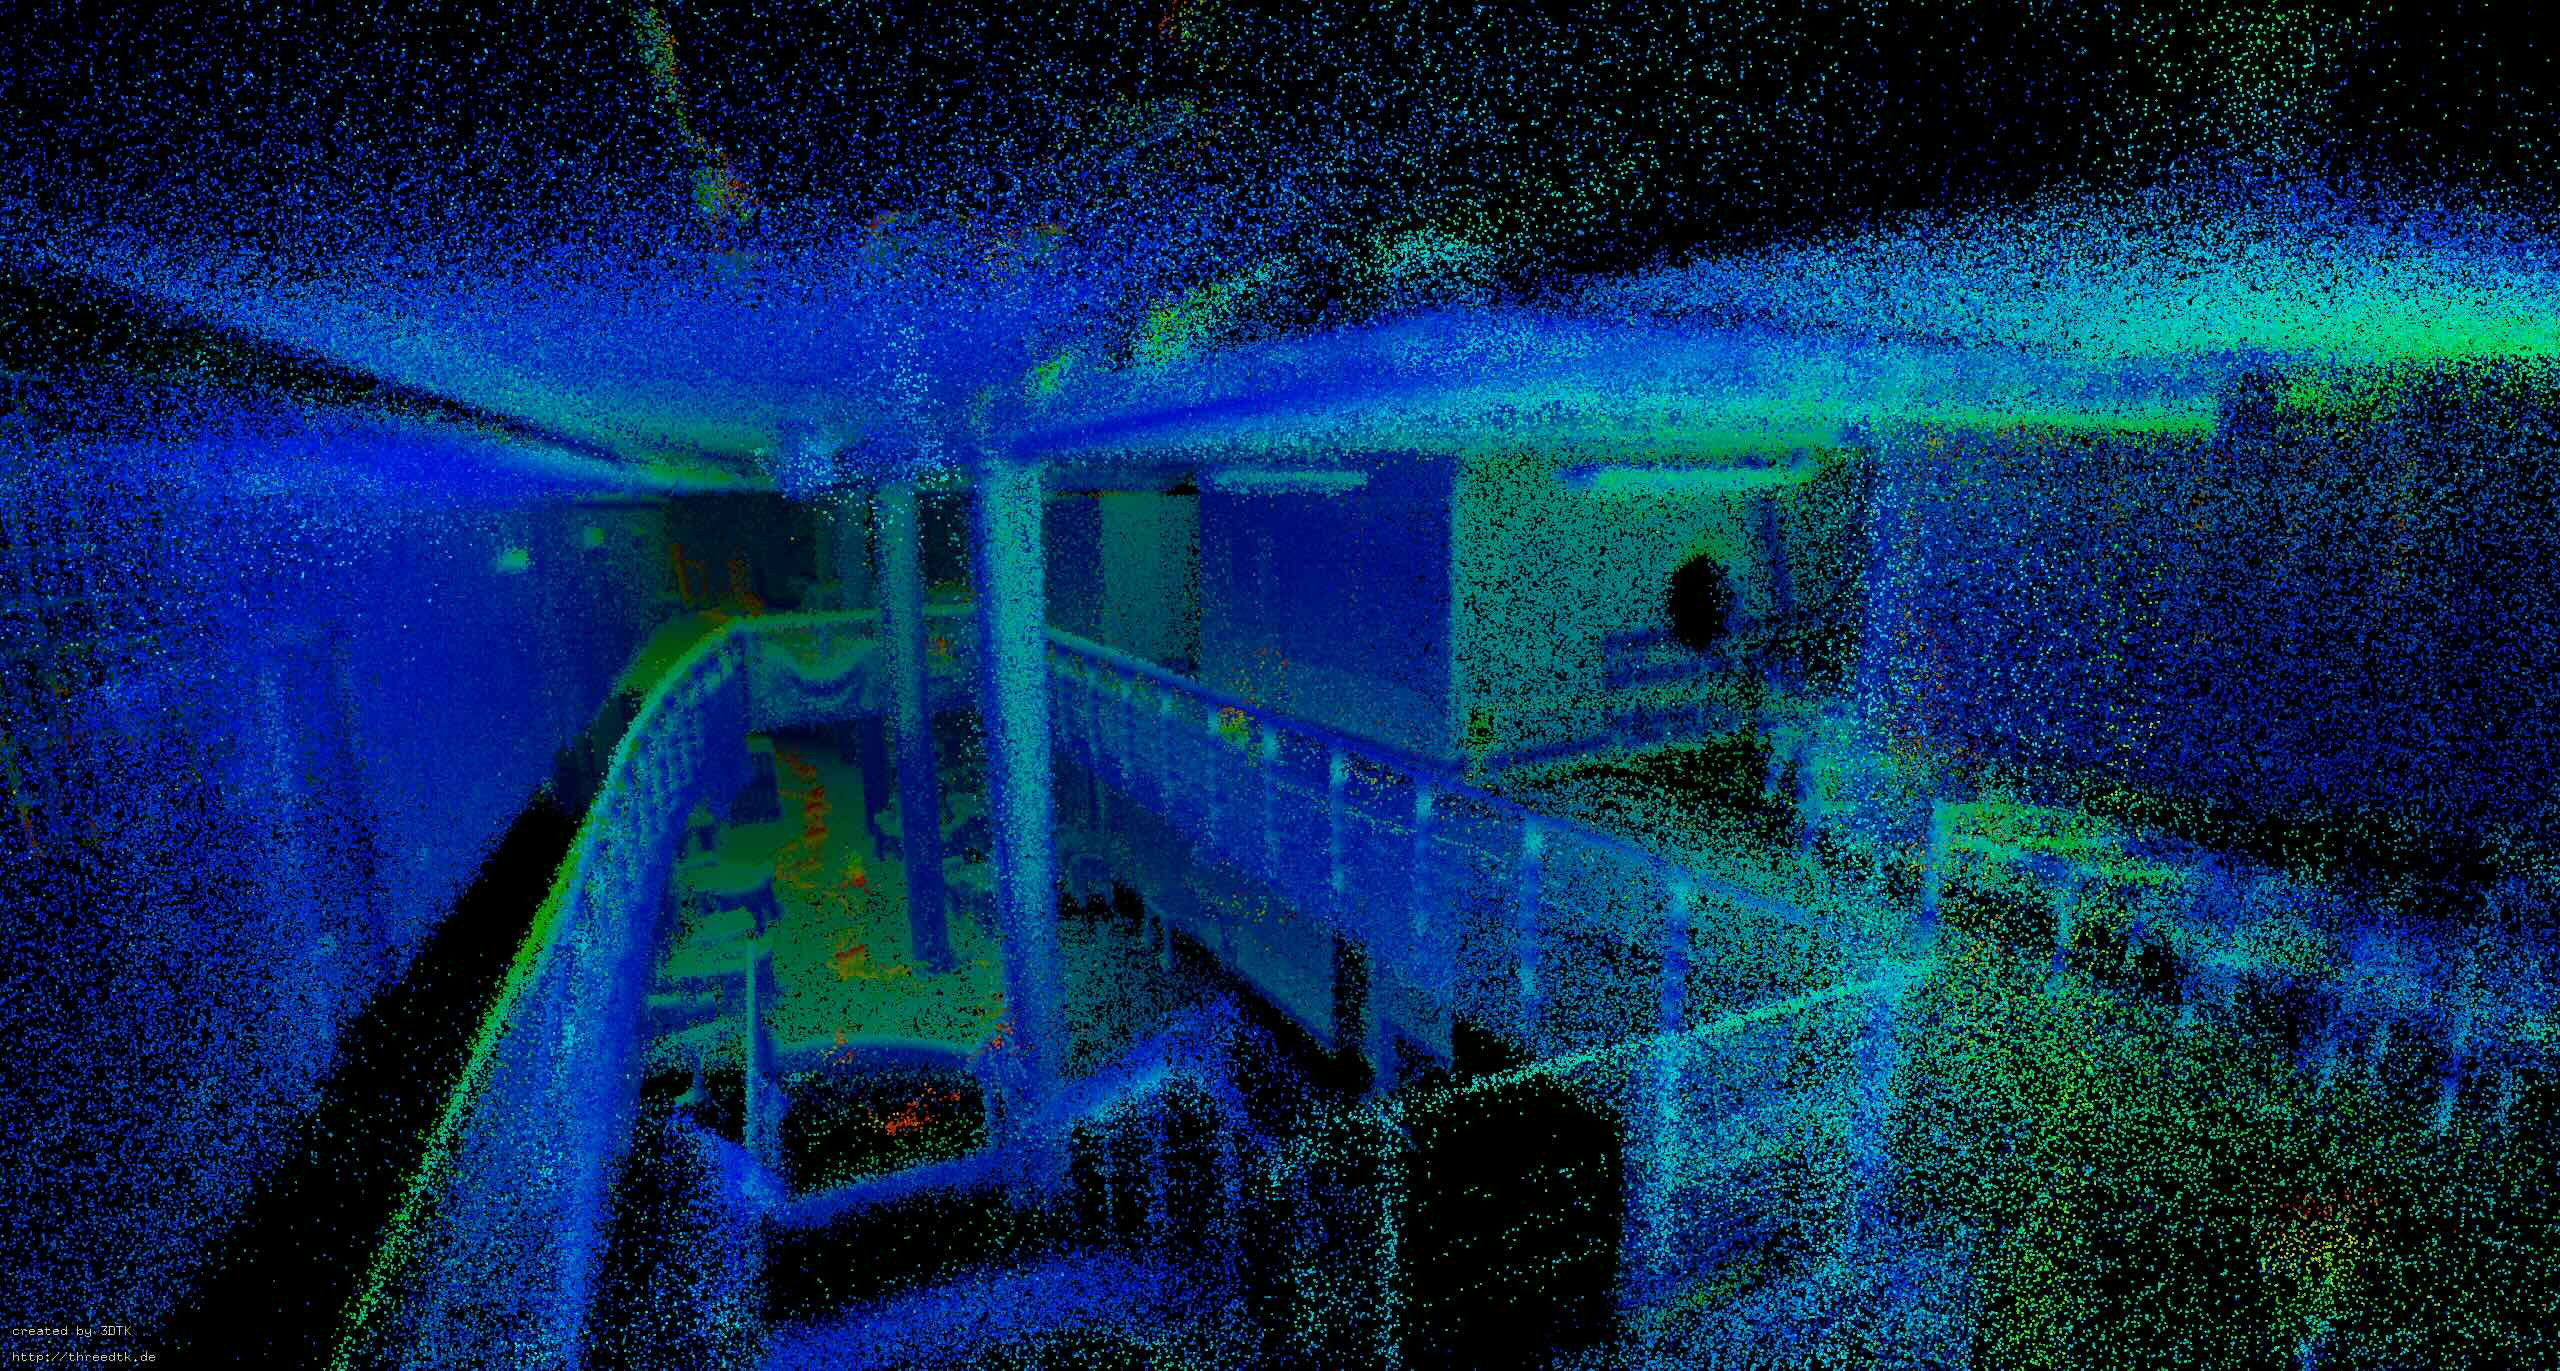
\includegraphics[width=\textwidth]{pics/results_images/a_lio.jpg}
    \label{fig:results_act_lio}
\end{subfigure}

\begin{subfigure}{0.4\textwidth}
    \centering
    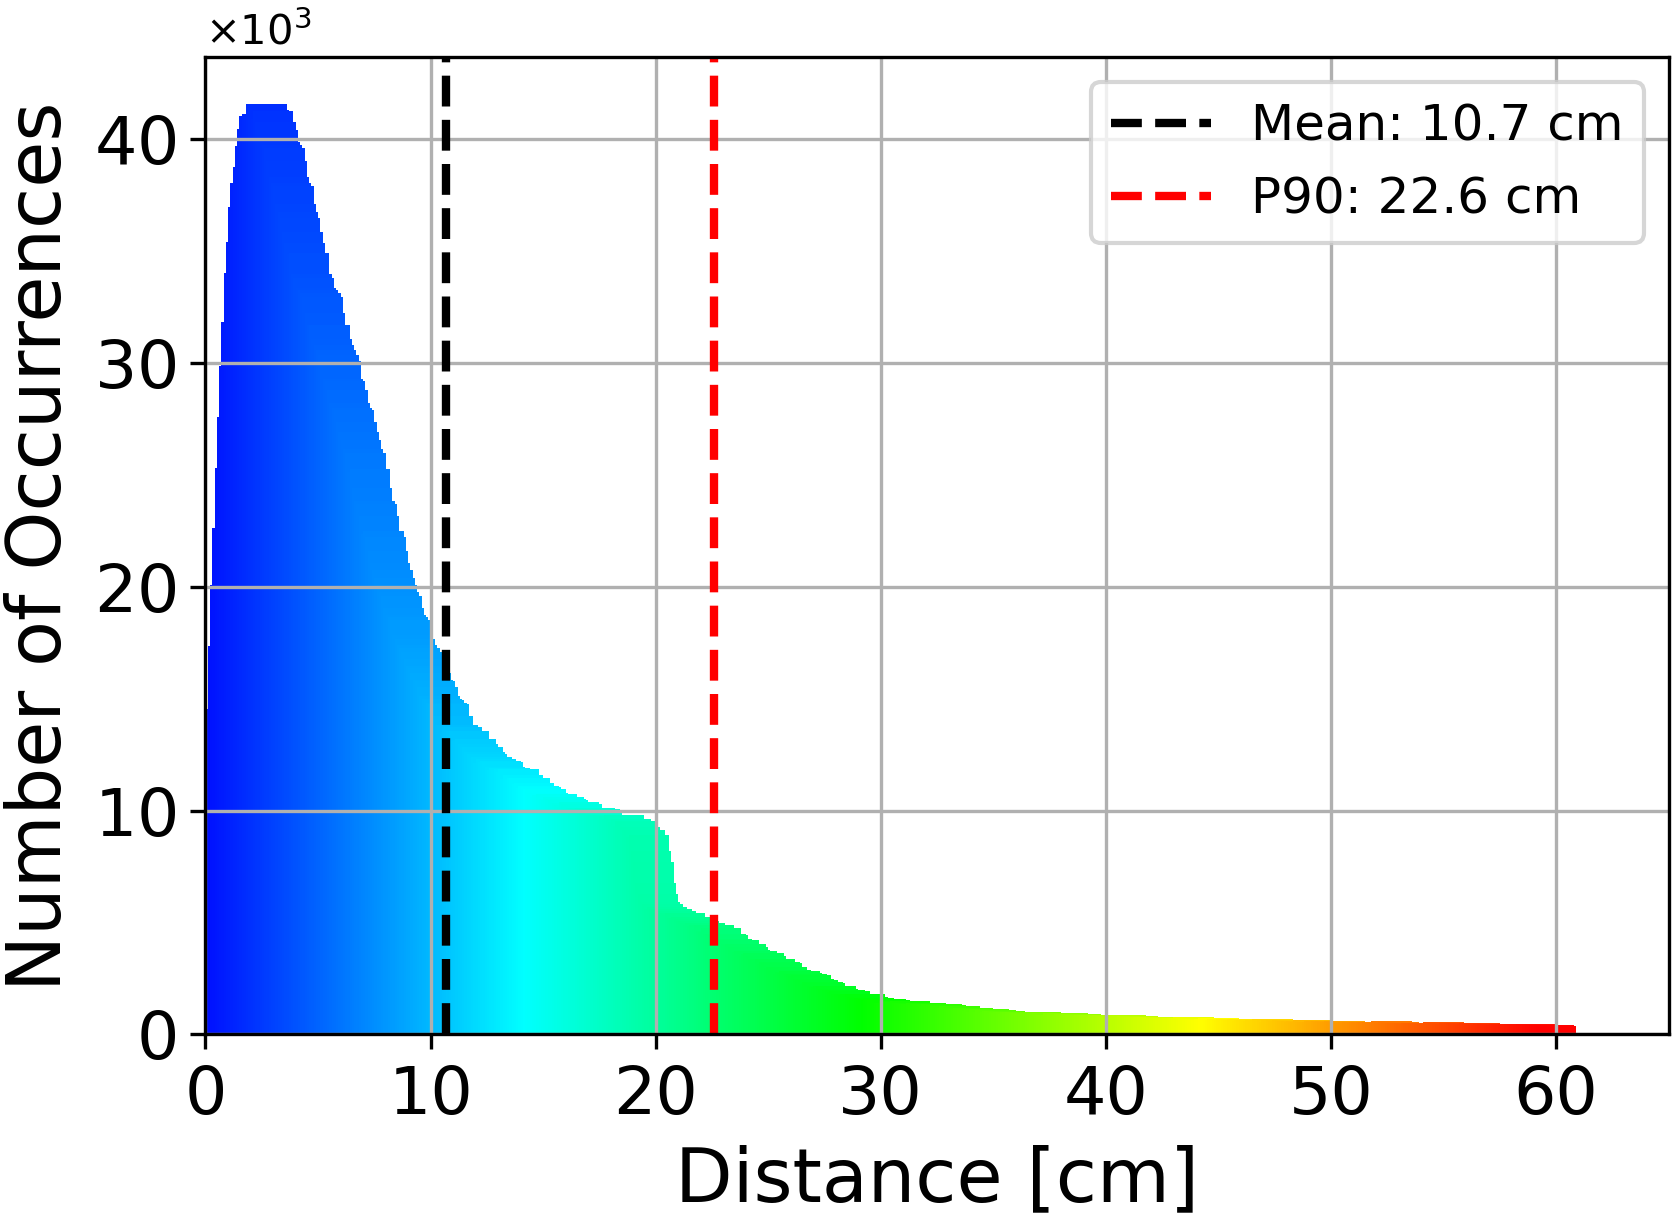
\includegraphics[width=\textwidth]{pics/histogram_results/histogram_cond_actuated_lio.png}
    \label{fig:hist_act_lio}
    \vspace{-5mm}
    \caption{Act. FAST-LIO2}
\end{subfigure}
\vspace{4mm}

\begin{subfigure}{0.4\textwidth}
    \centering
    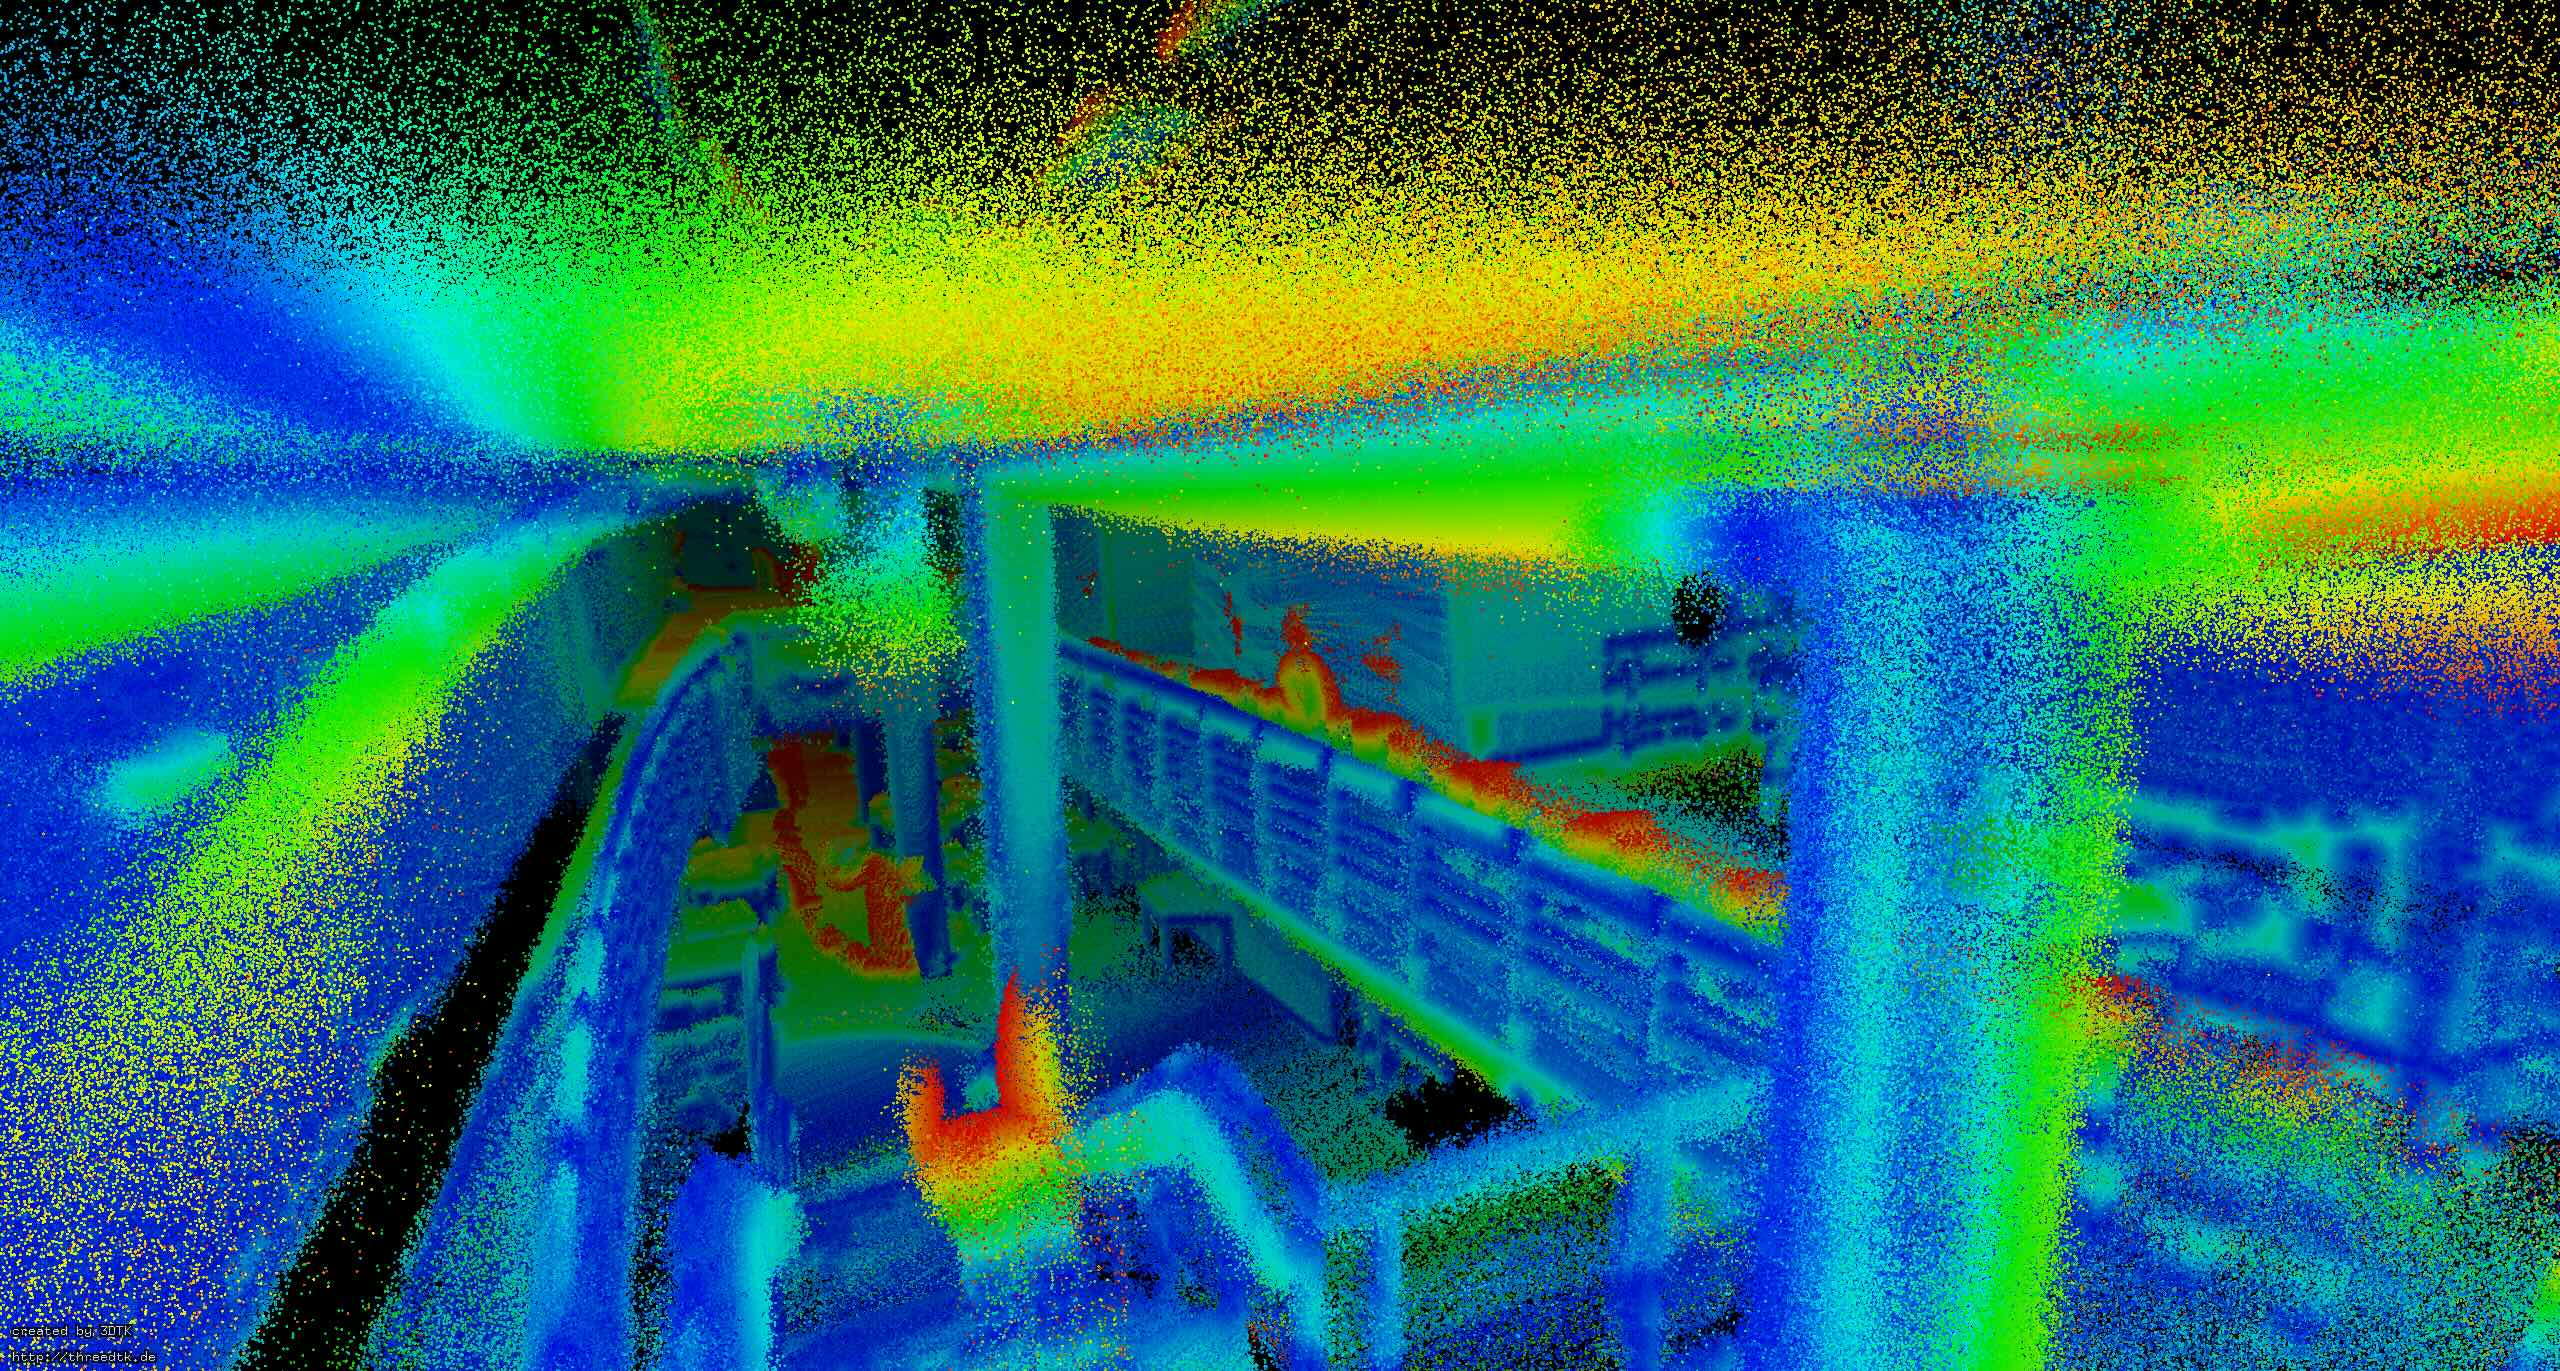
\includegraphics[width=\textwidth]{pics/results_images/a_dlio.jpg}
    \label{fig:results_act_dlio}
\end{subfigure}
\begin{subfigure}{0.4\textwidth}
    \centering
    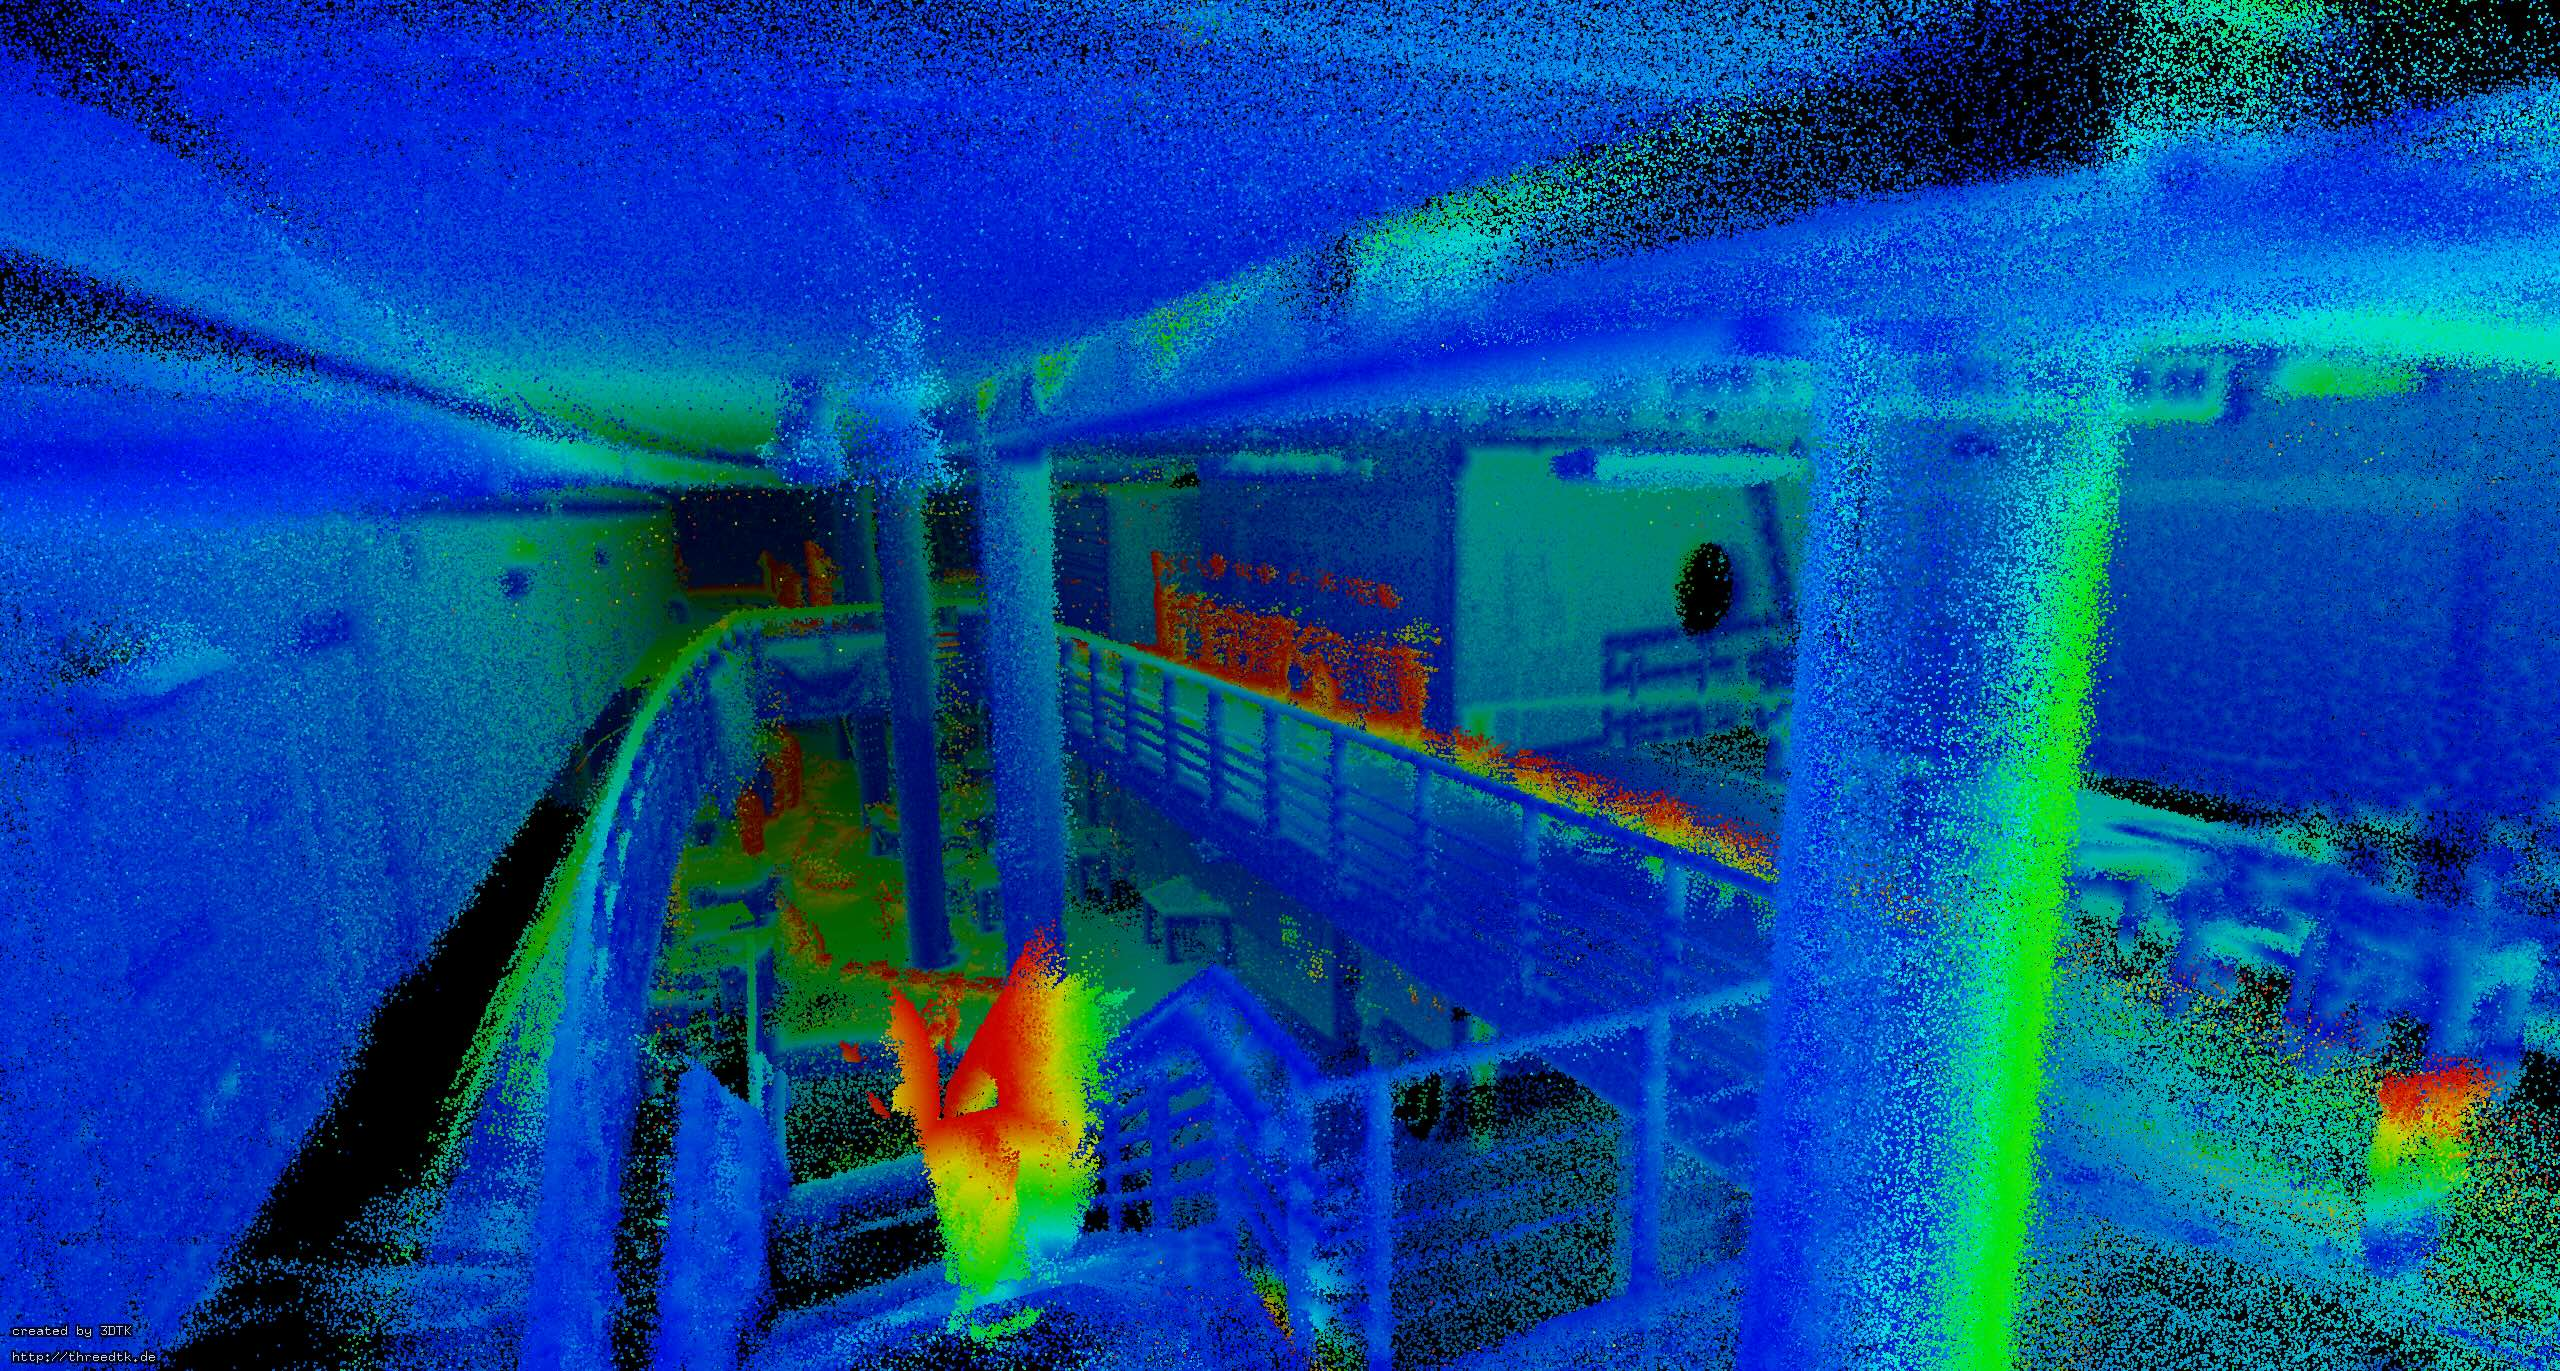
\includegraphics[width=\textwidth]{pics/results_images/a_livo.jpg}
    \label{fig:results_act_livo}
\end{subfigure}


\begin{subfigure}{0.4\textwidth}
    \centering
    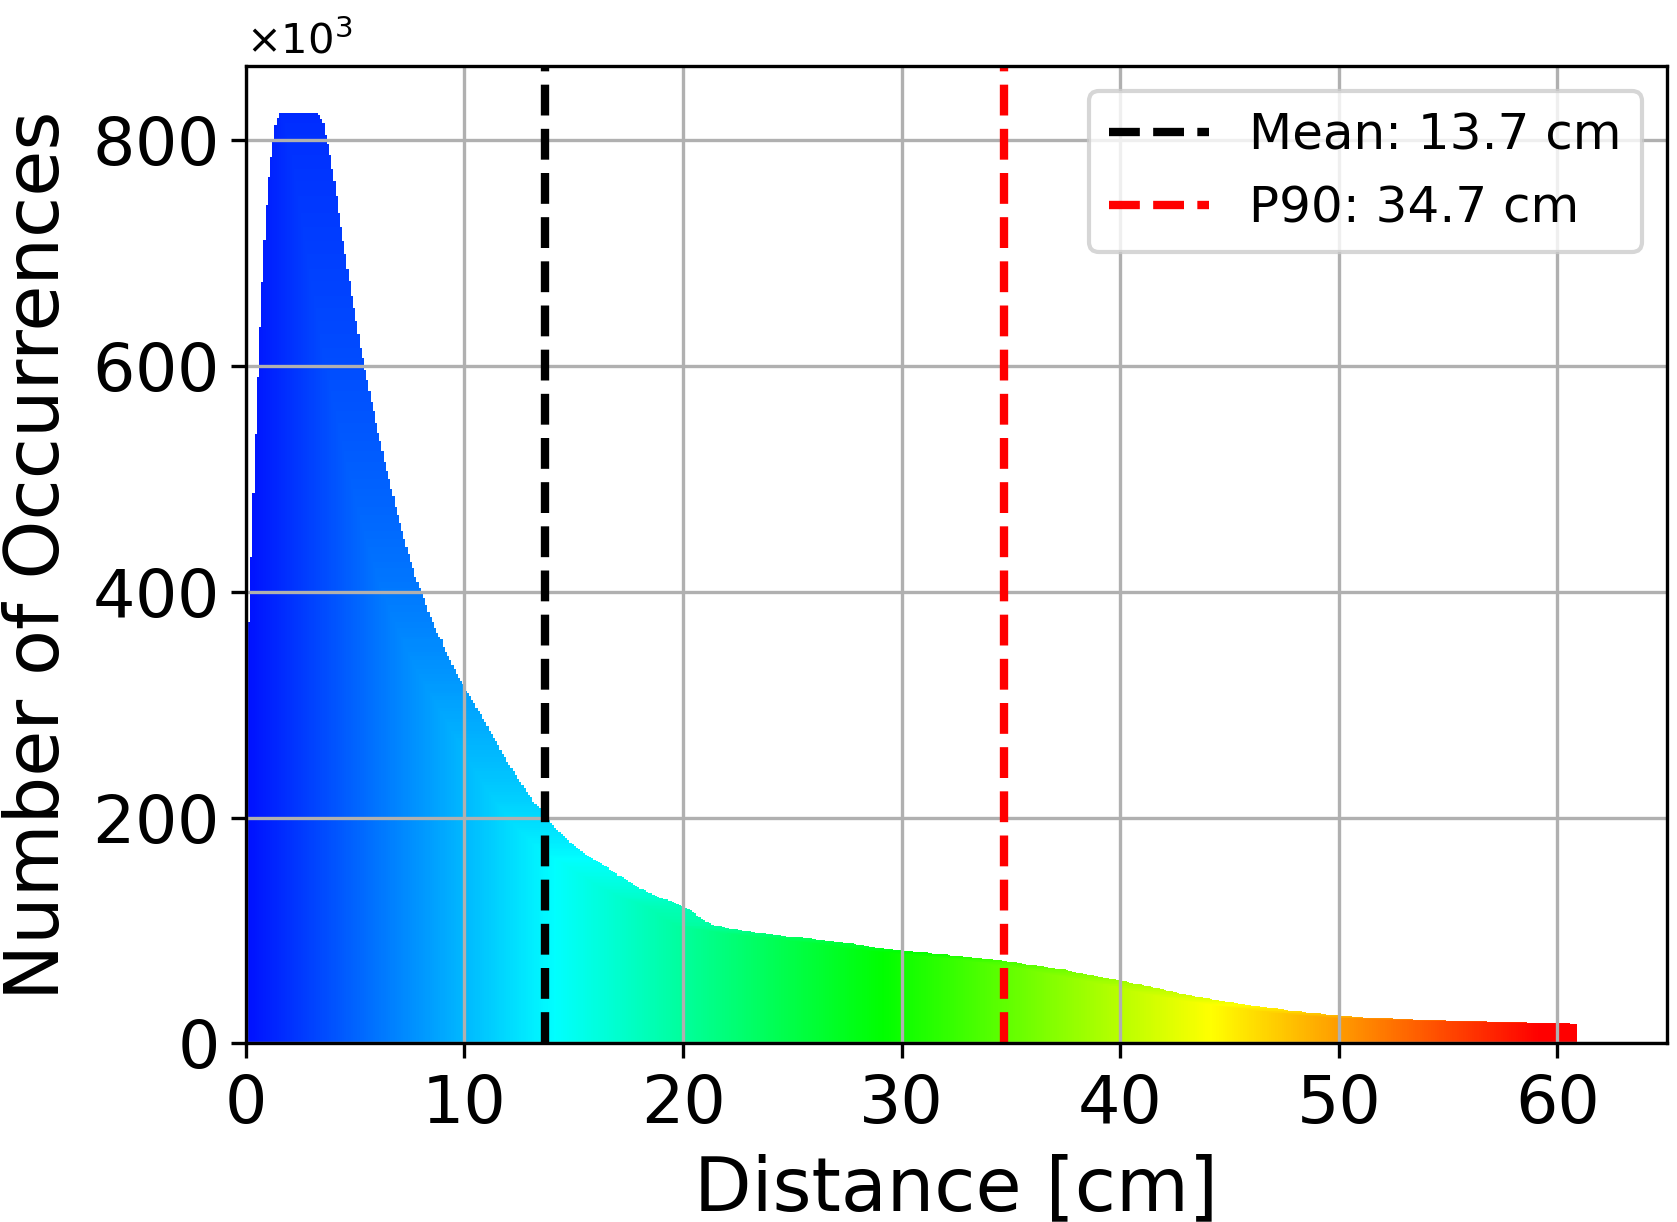
\includegraphics[width=\textwidth]{pics/histogram_results/histogram_cond_actuated_dlio.png}
    \caption{Act. DLIO}
    \label{fig:hist_act_dlio}
\end{subfigure}
\begin{subfigure}{0.4\textwidth}
    \centering
    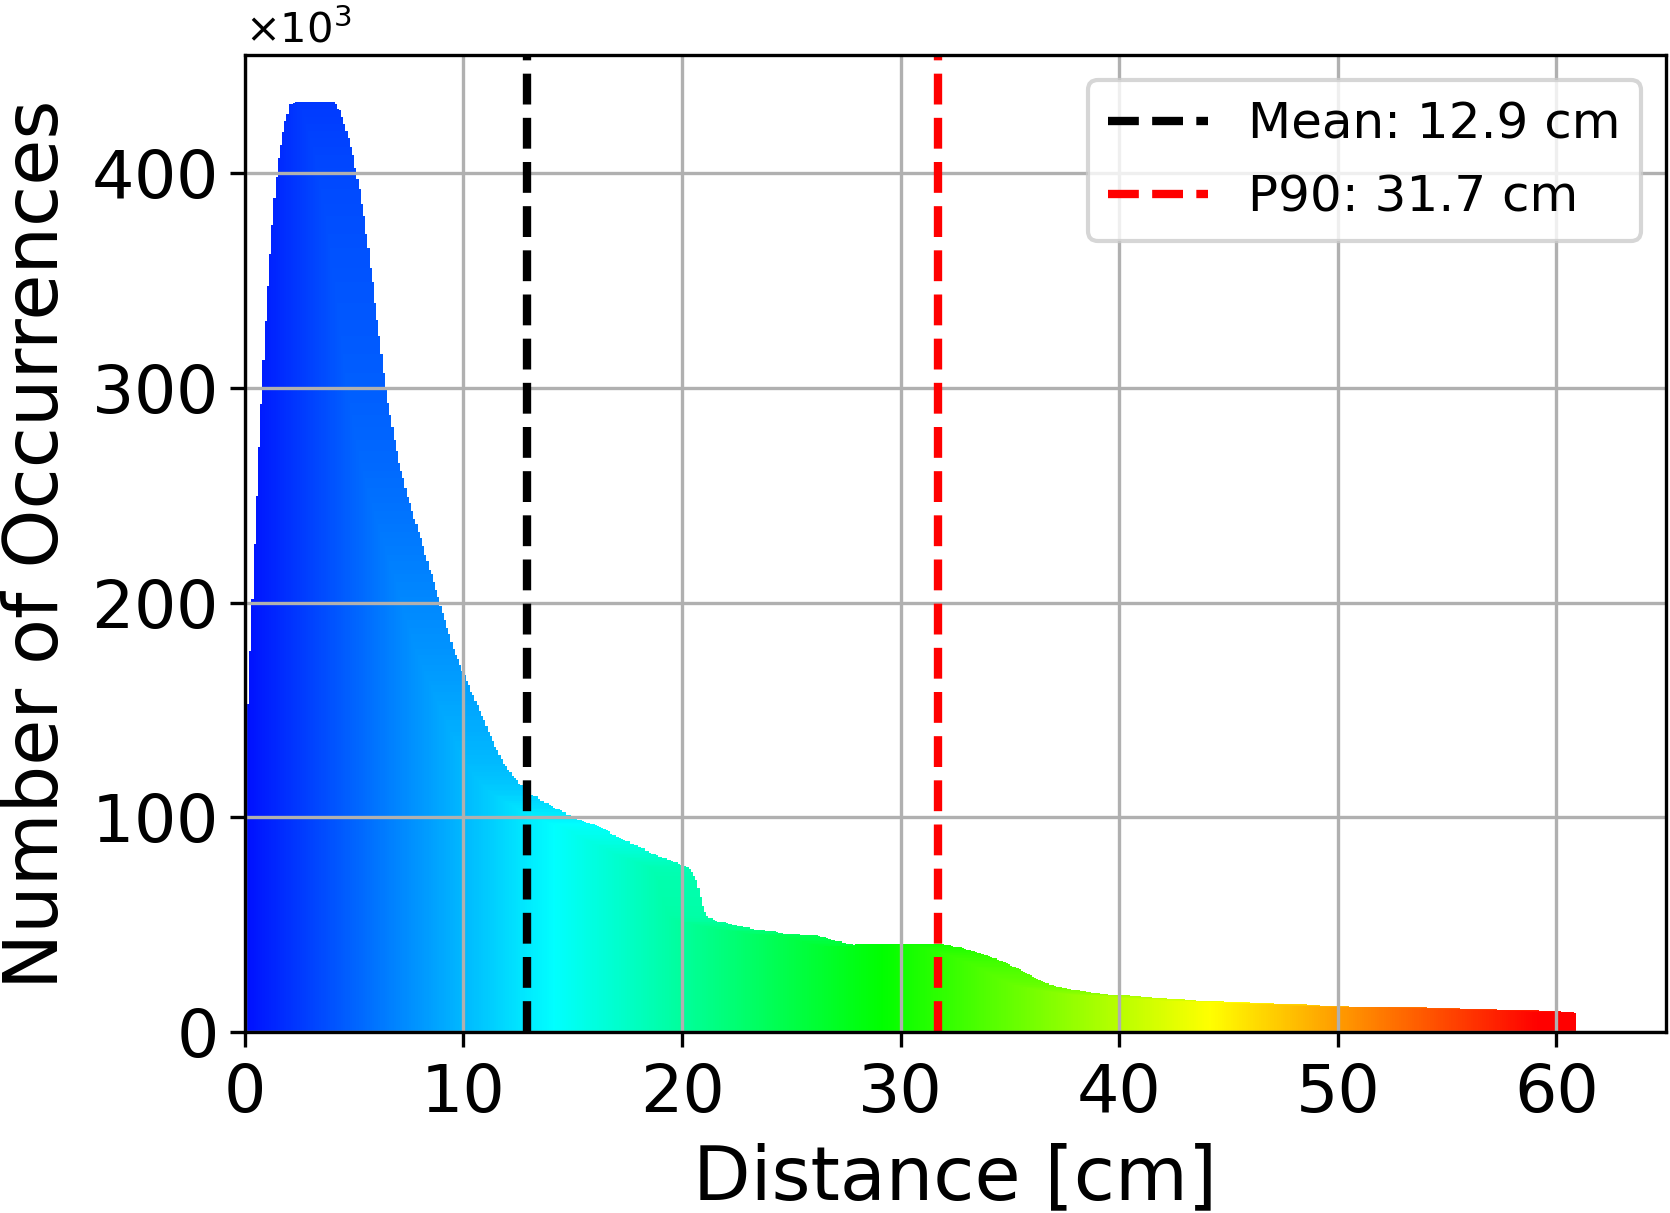
\includegraphics[width=\textwidth]{pics/histogram_results/histogram_cond_actuated_livo.png}
    \caption{Act. FAST-LIVO2}
    \label{fig:hist_act_livo}
\end{subfigure}
\begin{subfigure}{0.3\textwidth}
    \centering
    \includegraphics[width=\textwidth]{pics/histogram_results/hsv.png}
    \caption{Color Mapping}
    \label{fig:hsv}
\end{subfigure}
\vspace{2mm}
%tohere
    \caption{Point-cloud results and error distribution analysis (Part 2)}
    \label{fig:combined_results2}
\end{figure*}

\chapter{Conclusion}
In this thesis, we presented the design and evaluation of two spherical robots for 3D mapping applications: a non-actuated, and a self-actuated sphere. 
%The first prototype, a \SI{16}{\centi\meter} diameter non-actuated sphere, demonstrated effective mapping performance using state-of-the-art LIO algorithms on a compact and lightweight platform. 
The self-actuated sphere uses a pendulum-based locomotion mechanism, enabling controlled movement and stabilization in addition to mapping capabilities.
This is, to the best of our knowledge, the first prototype of a self-actuated spherical robot performing online LIO.   
The mapping accuracy of both systems was evaluated in a controlled indoor environment using ground truth point-clouds. 
The non-actuated sphere using FAST-LIO2 surprisingly achieved the lowest mean error and RMSE among all configurations.
We attribute this to the placement of the LiDAR sensor, which is closer to the center compared to the actuated sphere.
All tested algorithms produce bent point-clouds, and sometimes unrecoverable drift due to the rotationally aggressive motion of the system.  
%The actuated sphere showed strong potential for enhanced mobility and stability, marking a step forward in enabling more autonomous behaviors. 
%These results highlight the feasibility and promise of spherical robots for 3D mapping and real-time SLAM on resource-constrained platforms such as the Raspberry Pi 5.
%Only limited algorithmic configurations were explored in this work. 

In future work, we plan to incorporate motion models into the LIO algorithms that reflect the motion of the sphere better.
Furthermore, we want to explore alternative actuation mechanisms.
The actuated sphere, in particular, can be developed further for autonomous navigation and exploration tasks, leveraging its enhanced locomotion capabilities. 
Additionally, integrating higher-resolution LiDAR sensors—such as the Robosense Airy—could improve mapping quality without increasing sphere's form factor. 
Pose estimation accuracy was not directly addressed in this thesis, as establishing accurate ground truth trajectories would require a separate measurement setup, which was beyond the scope of this study.
Overall, this work contributes to the growing field of spherical robots and provides a foundation for future advancements in autonomous 3D mapping and mobile perception.
\chapter{Appendix}

\section{CAD Drawings}
\subsection{Non-Actuated Sphere}
\label{sec:non-actuated-sphere-drawings}
\clearpage % start of this subsection's drawings

\begin{figure}[H]
\centering
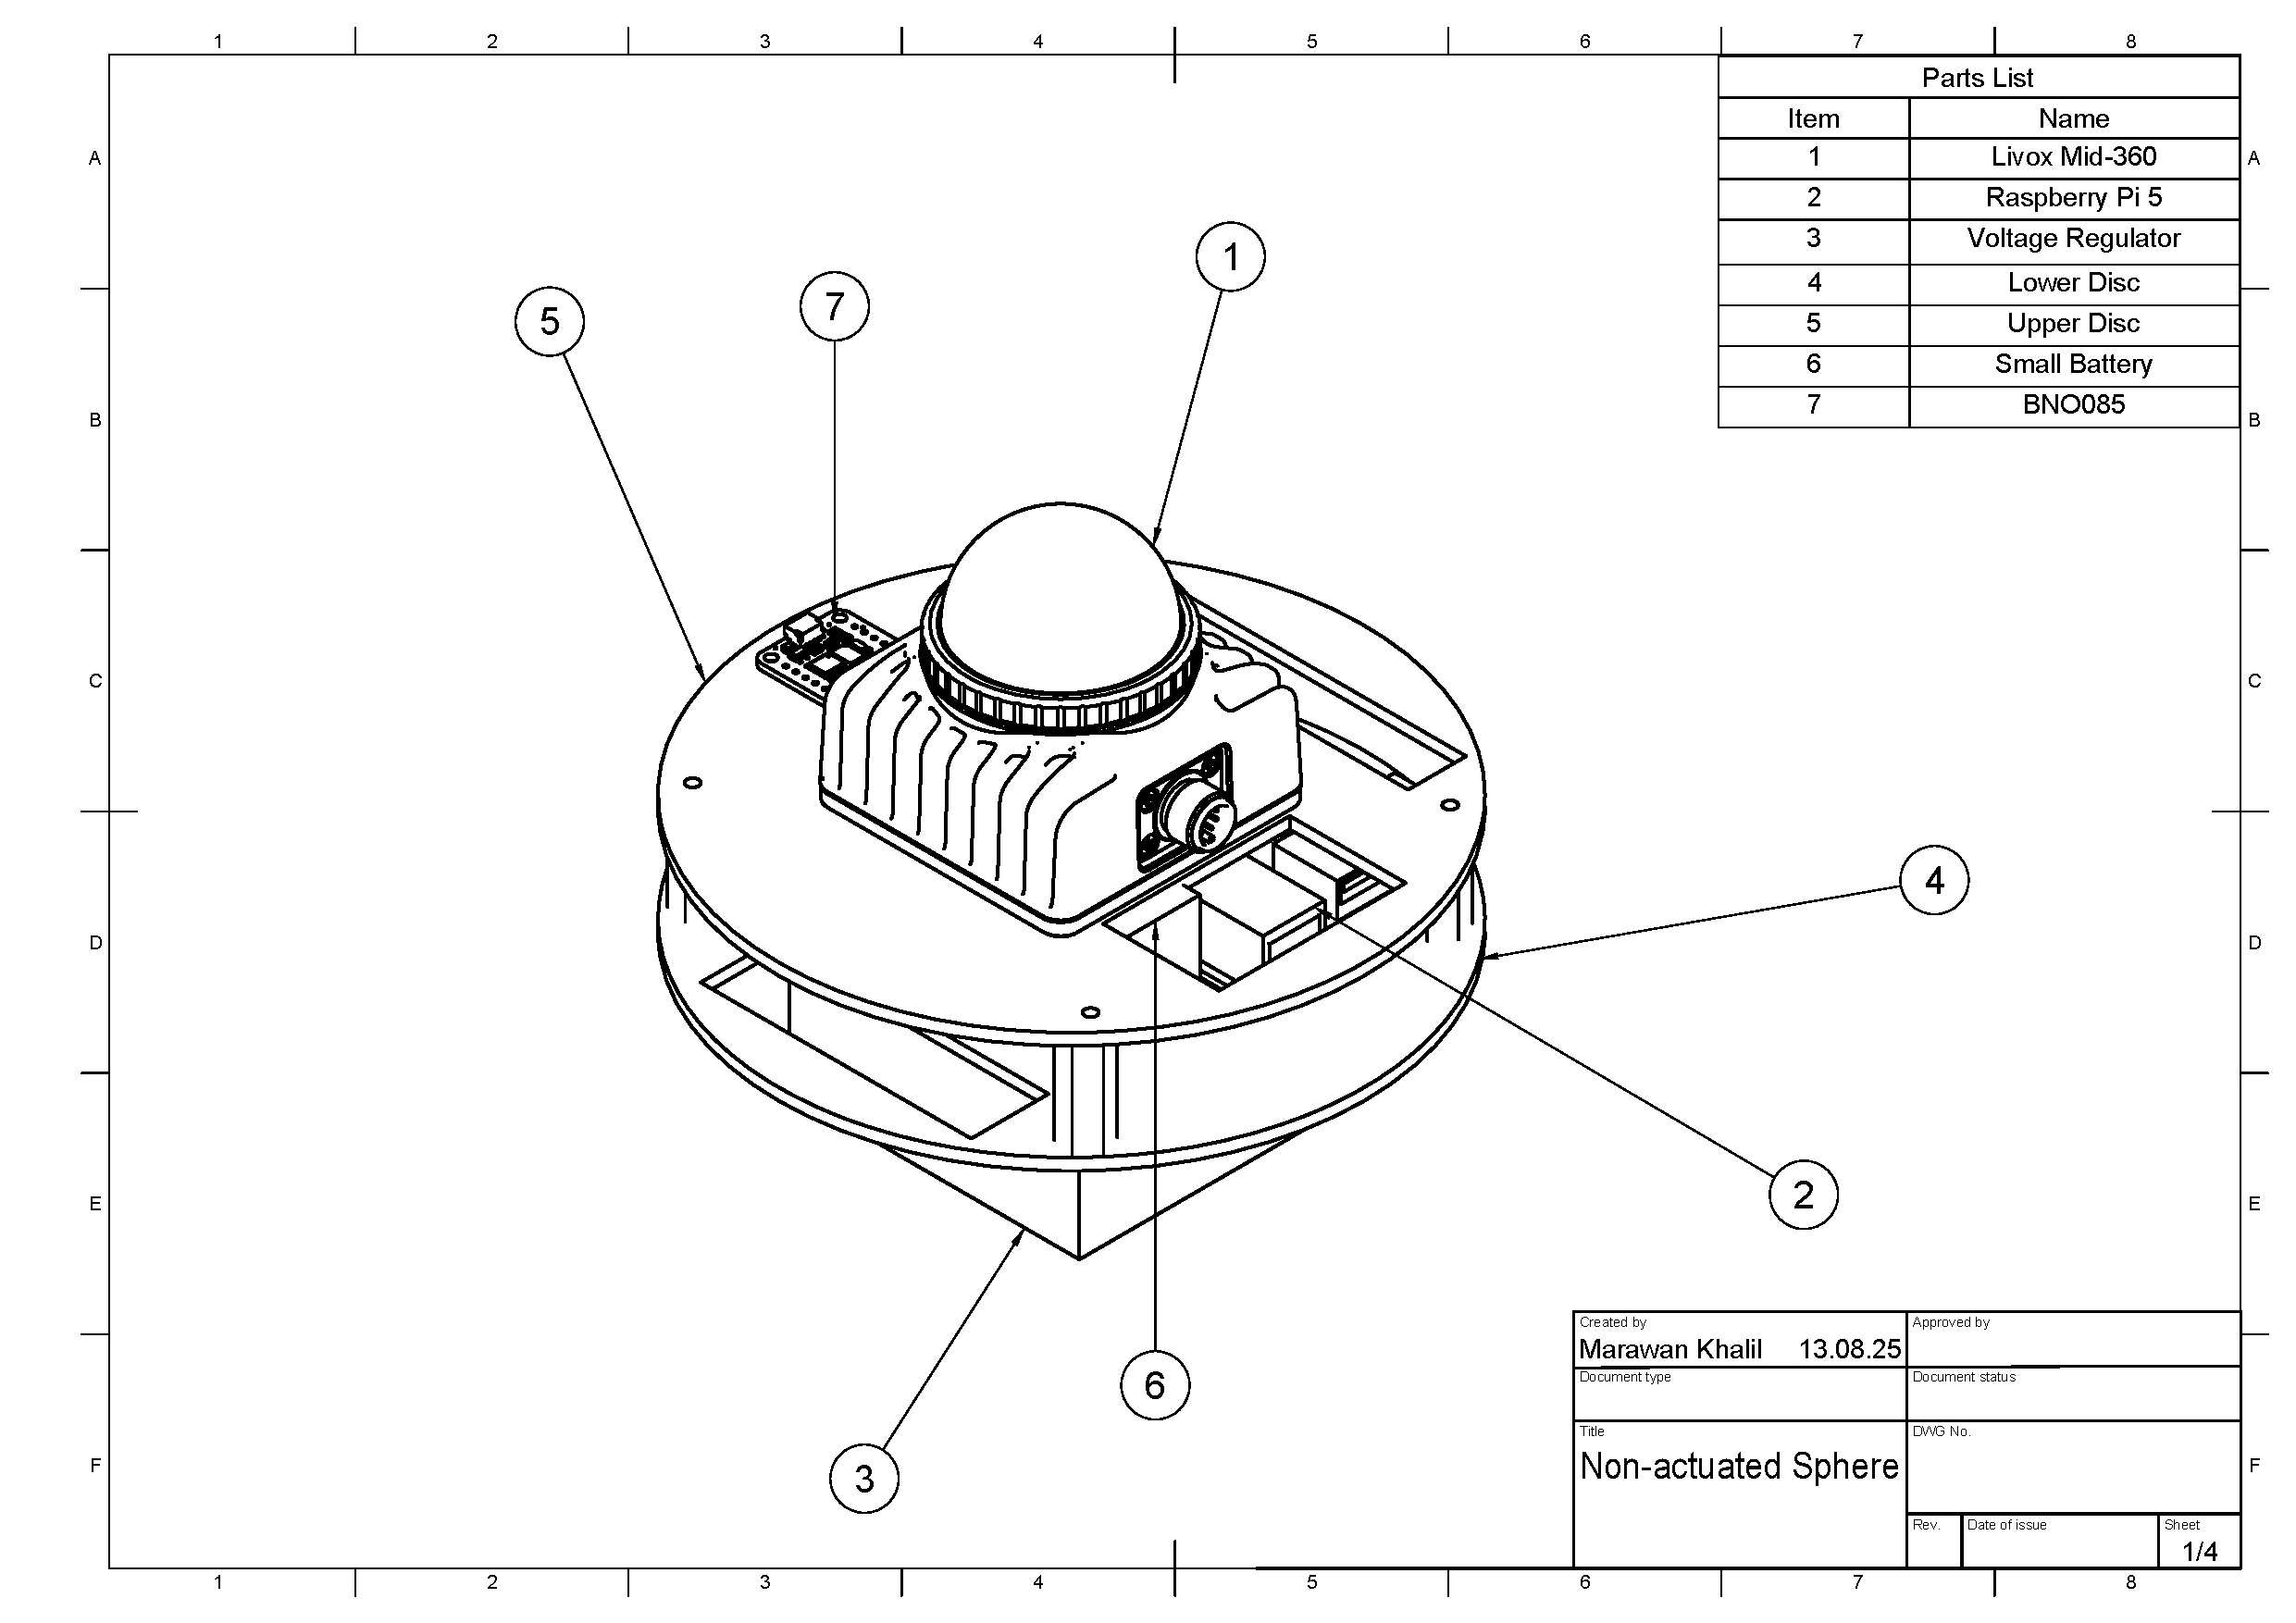
\includegraphics[width=0.82\textwidth,page=1]{pics/Non_actuated_Sphere_drawing.pdf}
\caption{Physical design and components}
\label{fig:system_page1}
\end{figure}

\begin{figure}[H]
\centering
\includegraphics[width=0.82\textwidth,page=2]{pics/Non_actuated_Sphere_drawing.pdf}
\caption{Orthographic projection of the non-actuated sphere}
\label{fig:system_page2}
\end{figure}

\begin{figure}[H]
\centering
\includegraphics[width=0.80\textwidth,page=3]{pics/Non_actuated_Sphere_drawing.pdf}
\caption{Upper disc dimensions}
\label{fig:system_page3}
\end{figure}

\begin{figure}[H]
\centering
\includegraphics[width=0.80\textwidth,page=4]{pics/Non_actuated_Sphere_drawing.pdf}
\caption{Lower disc dimensions}
\label{fig:system_page4}
\end{figure}

\clearpage % end of this subsection's drawings

\subsection{Actuated Sphere}
\label{sec:actuated-sphere-drawings}
\clearpage % end of this subsection's drawings

\begin{figure}
\centering
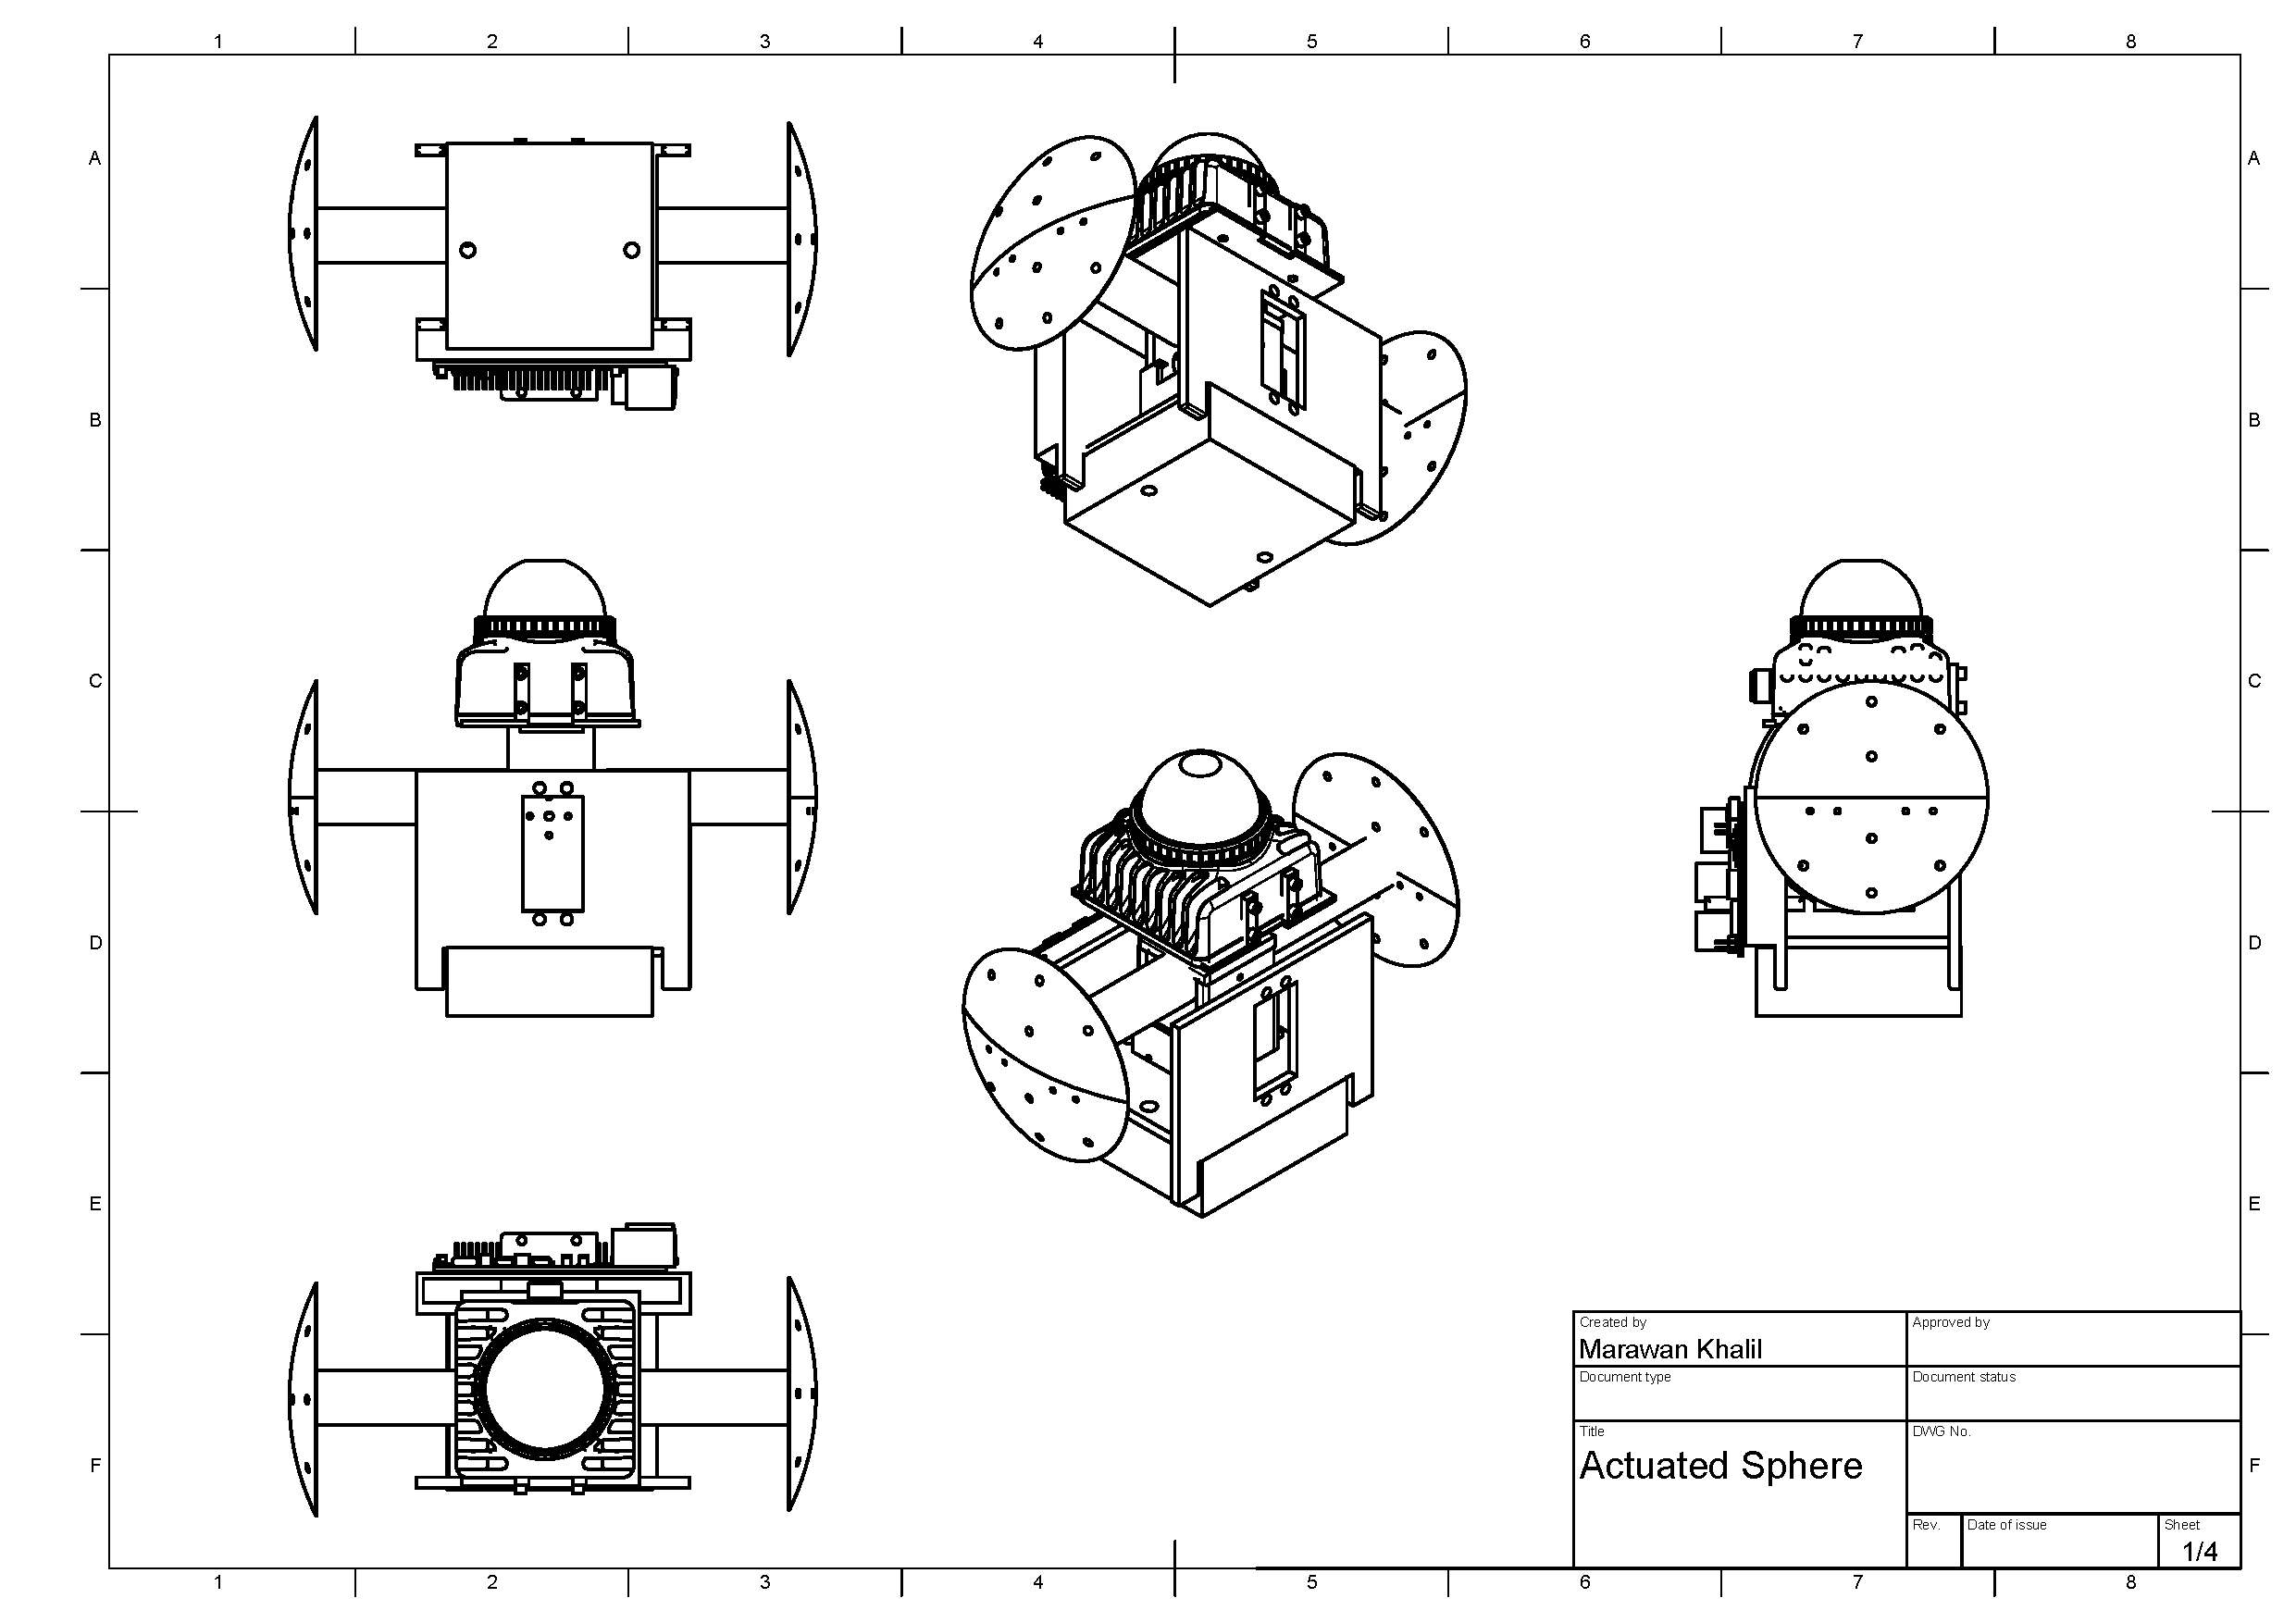
\includegraphics[width=0.80\textwidth,page=1]{pics/Actuated_Sphere_Drawing.pdf}
\caption{Physical design of the actuated sphere}
\label{fig:act_system_page1}
\end{figure}

\begin{figure}[H]
\centering
\includegraphics[width=0.80\textwidth,page=2]{pics/Actuated_Sphere_Drawing.pdf}
\caption{Orthographic projection of shell's hook}
\label{fig:act_system_page2}
\end{figure}

\begin{figure}[H]
\centering
\includegraphics[width=0.80\textwidth,page=3]{pics/Actuated_Sphere_Drawing.pdf}
\caption{Orthographic projection of the main body}
\label{fig:act_system_page3}
\end{figure}

\begin{figure}[H]
\centering
\includegraphics[width=0.80\textwidth,page=4]{pics/Actuated_Sphere_Drawing.pdf}
\caption{Orthographic projection of internal servo case}
\label{fig:act_system_page4}
\end{figure}

\clearpage

\begin{figure}[H]
\centering
\includegraphics[width=0.80\textwidth,page=5]{pics/Actuated_Sphere_Drawing2.pdf}
\caption{Orthographic projection of LiDAR}
\label{fig:act_system_page5}
\end{figure}



% DON'T set \bibliographystyle here -- use the documentclass option instead
\bibliography{papers}

\closing %%%%%%%%%%%%%%%%%%%%%%%%%%%%%%

\end{document}
